% @HEADER
% ***********************************************************************
%
%            Trilinos: An Object-Oriented Solver Framework
%                 Copyright (2001) Sandia Corporation
%
% Under terms of Contract DE-AC04-94AL85000, there is a non-exclusive
% license for use of this work by or on behalf of the U.S. Government.
%
% This library is free software; you can redistribute it and/or modify
% it under the terms of the GNU Lesser General Public License as
% published by the Free Software Foundation; either version 2.1 of the
% License, or (at your option) any later version.
%
% This library is distributed in the hope that it will be useful, but
% WITHOUT ANY WARRANTY; without even the implied warranty of
% MERCHANTABILITY or FITNESS FOR A PARTICULAR PURPOSE.  See the GNU
% Lesser General Public License for more details.
%
% You should have received a copy of the GNU Lesser General Public
% License along with this library; if not, write to the Free Software
% Foundation, Inc., 59 Temple Place, Suite 330, Boston, MA 02111-1307
% USA
% Questions? Contact Michael A. Heroux (maherou@sandia.gov)
%
% ***********************************************************************
% @HEADER

\documentclass[final]{colabarticle}
\usepackage{fancyhdr} %Declares the package fancyhdr
\pagestyle{fancy} %Forces the page to use the fancy template
\usepackage{graphicx}
\usepackage{a4wide}
\usepackage{amsmath,amsfonts,amsthm}
\usepackage{amssymb}
\usepackage{a4wide}
\usepackage{eepic}
\usepackage{epsfig}
\usepackage{graphicx}
\usepackage{here}
\usepackage{latexsym}
\usepackage{natbib}
\usepackage{subfigure}
\usepackage{tabularx}
\usepackage{wrapfig}
\usepackage{makeidx}
\usepackage{graphicx}
\usepackage{psboxit}
\usepackage{color}

%Postscript Font Name                   Name to use in
%                                       \newfont command
%                                       (dvips syntax)
%----------------------------------------------------------
%AvanteGarde-Book                       rpagk
%AvanteGarde-BookOblique                        rpagko
%AvanteGarde-Demi                       rpagd
%AvanteGarde-DemiOblique                        rpagdo
%Bookman-Demi                           rpbkd
%Bookman-Light                          rpbkl
%Courier                                        rpcrr
%Courier-Bold                           rpcrb
%Courier-Oblique                                rpcrro
%Courier-BoldOblique                    rpcrbo
%Helvetica                              rphvr
%Helvetica-Bold                         rphvb
%Helvetic-Oblique                       rphvro
%Helvetica-BoldOblique                  rphvbo
%NewCenturySchlbk-Roman                 rpncr
%NewCenturySchlbk-Italic                        rpncri
%NewCenturySchlbk-Bold                  rpncb
%NewCenturySchlbk-BoldItalic            rpncbi
%Palatino                               rpplr
%Palatino-Bold                          rpplb
%Palatino-Italic                                rpplri
%Palatino-Oblique                       rpplro
%Times-Roman                            rptmr
%Times-Bold                             rptmb
%Times-Italic                           rptmri
%Times-BoldItalic                       rptmbi
%Zapf Chancery Medium Italic            rpzcmi

%\newfont{\ridiculous}{rpagd scaled 10000}
\newfont{\supergrand}{rpncb scaled 8000}
\definecolor{mygray}{rgb}{0.8,0.8,0.8}

\makeatletter
\def\@makechapterhead#1{%
  {
    \vspace*{-1.5cm}
    \begin{center}
      \hfill
      \begin{tabular}{c}
        
\includegraphics[width=3.2cm]{chapterbox}\\[-2.7cm]
        \color{white}{\supergrand\thechapter}
      \end{tabular}
    \end{center}
    \vspace*{0.5cm}
    \begin{flushleft}
      \Huge\sf\textbf{#1}
    \end{flushleft}
    \vspace*{1cm}
  }}

\def\imp#1{\textbf{#1}}

%%%\usepackage{newcent}
%%%\usepackage{fancycha}

\def\choicebox#1#2{\noindent$\hphantom{th}$\parbox[t]{1.8in}{\sf
#1}\parbox[t]{4.5in}{#2}\\[0.8em]}

\newcommand{\TriExe}[1]{{\tt didasko/examples/#1}}

\newcommand{\ChapterAuthors}[1]{{\vspace*{-0.8cm}{\sl #1 } \bigskip}}

\newenvironment{introchapter}
{ \begin{center} \begin{tabular}{|p{0.1cm} p{14cm} p{0.1cm}|} &
  \fontfamily{cmss}\selectfont  }
{  & \\ \end{tabular} \end{center} }

\newcommand{\Trilinos}{Trilinos}
\newcommand{\TrilinosTM}{Trilinos \copyright}

\newtheorem{remark}{Remark}

%-------------------------------------------------------------------------------
%  title page
%-------------------------------------------------------------------------------
\title{\textbf{\resizebox{10cm}{!}{Trilinos Tutorial}}\vspace{5mm}}
\subtitle{
  \\
  \vspace*{4mm}
  \Large For Trilinos Release 10.0 \\
  \vspace*{5mm}
  \noindent
  Sandia Report SAND2004-2189,
  September 2004,
  Unlimited Release \\
  \vspace*{5mm}
  \noindent
  Last updated October 2009 \\
\vspace{6cm}\\
\\ \vspace{0mm}
\hspace*{1cm} Marzio Sala \\
\\ \vspace{0mm}
\hspace*{1cm} Michael A. Heroux\\
\\ \vspace{0mm}
\hspace*{1cm} David M. Day\\
\\ \vspace{0mm}
\hspace*{1cm} James M. Willenbring\\
\\ \vspace{0mm}
\hspace*{1cm} \normalsize (Editors) \\
\vspace*{1cm}
\vfill

\includegraphics[height=1.5cm]{snllineblk}  \hfill

\includegraphics[height=1.5cm]{DOEbwlogo}  \\
Sandia is a multiprogram laboratory operated by Sandia Corporation,
a Lockheed Martin Company, for the United States Department of Energy's
National Nuclear Security Administration under Contract DE-AC04-94-AL85000.
Approved for public release; further dissemination unlimited.
}

%\institute{http://www.colab.ethz.ch}
 \correspondingauthor{ }
 \http{www.sandia.gov}
%\email{marzio@inf.ethz.ch}

\COLABreportdate{February 2006}

\pagestyle{fancy}

\fancyhf{}
\fancyhead[LE,RO]{\thepage}
\fancyhead[RE]{\sf \nouppercase{\leftmark}}
\fancyhead[LO]{\sf \nouppercase \rightmark}
\renewcommand{\headrulewidth}{0.5pt}
\begin{document}

\maketitle

\chapter*{Preface}
  The Trilinos Project is an effort to facilitate the design,
  development, integration and ongoing support of mathematical software
  libraries.  The goal of the Trilinos Project is to develop algorithms
  and enabling technologies within an object-oriented software
  framework for the solution of large-scale, complex multiphysics
  engineering and scientific applications. There is an emphasis is on 
  developing robust, scalable algorithms in a software framework, using
  abstract interfaces for flexible interoperability of components while
  providing a full-featured set of concrete classes that implement all
  the abstract interfaces.

  \medskip

  This document introduces the use of \Trilinos{}, Release 10.0 and
  subsequent minor releases 10.0.X.  The
  presented material includes, among others, the definition of
  distributed matrices and vectors with Epetra, the iterative solution
  of linear systems with AztecOO, incomplete factorizations with IFPACK,
  multilevel and domain decomposition preconditioners with ML, direct
  solution of linear system with Amesos,
  eigenvalues and eigenvectors computations with Anasazi,
  and iterative solution of nonlinear systems with NOX.

  The tutorial is a self-contained introduction, intented to help
  computational scientists effectively apply the appropriate Trilinos
  package to their applications. Basic examples are presented that are
  fit to be imitated.

  \medskip

  This document is a companion to the Trilinos User's
  Guide~\cite{Trilinos-Users-Guide} and Trilinos Development
  Guides~\cite{Trilinos-Dev-Guide,Trilinos-Dev-Guide-II}. Please note
  that the documentation included in each of the Trilinos' packages is
  of fundamental importance.

  \bigskip

  The developers of each Trilinos' package are acknowledged for providing
  excellent documentation and examples (and the code itself!),
  without which this document would have never been possible.  We also
  acknowledge the support of the ASCI and LDRD programs that funded
  development of Trilinos, and the support of D-INFK department of the ETH
  Z\"urich.

  \smallskip

  Oscar Chinellato (ETHZ/ICoS) and Jens Walter (ETHZ/ICOS) are acknowledged
  for the \LaTeX\ macros and styles used to format this document.

  \vspace*{1cm}

  \hfill Marzio Sala

  \hfill Micheal Heroux

  \hfill David Day

  \hfill James Willenbring

\clearpage

\tableofcontents

\clearpage

%@HEADER
% ************************************************************************
% 
%          Trilinos: An Object-Oriented Solver Framework
%              Copyright (2001) Sandia Corporation
% 
% Under terms of Contract DE-AC04-94AL85000, there is a non-exclusive
% license for use of this work by or on behalf of the U.S. Government.
% 
% This program is free software; you can redistribute it and/or modify
% it under the terms of the GNU General Public License as published by
% the Free Software Foundation; either version 2, or (at your option)
% any later version.
%   
% This program is distributed in the hope that it will be useful, but
% WITHOUT ANY WARRANTY; without even the implied warranty of
% MERCHANTABILITY or FITNESS FOR A PARTICULAR PURPOSE.  See the GNU
% General Public License for more details.
%   
% You should have received a copy of the GNU General Public License
% along with this program; if not, write to the Free Software
% Foundation, Inc., 675 Mass Ave, Cambridge, MA 02139, USA.
% 
% Questions? Contact Michael A. Heroux (maherou@sandia.gov)
% 
% ************************************************************************
%@HEADER

\section{Introduction}

The Trilinos Project is an effort to facilitate the design, development,
integration and ongoing support of mathematical software libraries. In
particular, the goal of the Trilinos Project is develop parallel solver
algorithms and libraries within an object-oriented software framework
for the solution of large-scale, complex multiphysics engineering and
scientific applications. The emphasis is on developing robust, scalable
algorithm in a software framework, using abstract interfaces for
flexible interoperability of components while providing a full-featured
set of concrete classes that implement all abstract interfaces.

%%%
%%%
%%%

\subsection{Getting Started with Trilinos}
\label{sec:getting}

The Trilinos Project uses a two-level software structure designed around
collections of packages. A Trilinos package is an integral unit, usually
developed to solve a specific task, by a (relatively) small group of
expert of the field.  Packages exist underneath the Trilinos top level,
which provides a common look-and-feel. Each package has its own
structure, documentation and set of examples. In principle, Trilinos
packages can live independently. However, each package is even more
valuable when combined with other Trilinos packages.

\smallskip

Trilinos is a large software project, and currently about twenty
packages are included. Fully understanding all the functionalities of
the Trilinos packages requires time. The entire set of packages covers a
wide range of numerical methods for large scale computing. Some packages
are focused on the development of computational schemes, like for
instance the solution of linear and nonlinear systems, to the definition
of parallel preconditioners for Krylov methods, eigenvalue computation.
Other packages are more focused on implementation issues (like
definition of matrices and vectors, abstract classes for linear
operators). The first Chapters of this tutorial will be focused on
implementation issues, while the last Chapters will have a more
``mathematical'' taste.

Each package offers sophisticated features, that cannot be ``unleashed''
at a very first usage. For each package, wew will outline only the basic
features, and we refer to the documentation of each package for a more
involved usage. Our goal is to present enough material so that the
reader can successfully use the described packages.  In fact, for new
users, it is neither easy, nor necessary, to manage all the Trilinos
functionalities. At the beginning, it is more important for them to
understand how to manage the basic classes, such as vector, matrix and
linear system classes. However, it is clear that for a fine-tuning, the
reader will have to look through each package's documentation and
examples.

\medskip

Although all packages have the same importance in the Trilinos
structure, a typical user will probably --- at least at the beginning
--- make use of the following packages:
\begin{itemize} 
\item {\bf Epetra}. This package defines the basic classes for
  distributed matrices and vectors, linear operators and linear
  problems. Epetra classes are the common language spoken by all the
  Trilinos packages (even if some of them can ``speak'' other
  languages). Each Trilinos package is able to accept in input Epetra
  objects. This allows powerful combinations among the various Trilinos
  functionalities.
\item {\bf AztecOO}. This is a linear solve package based on
  preconditioned Krylov methods. It supports all the Aztec interfaces
  and functionality, but also provides significant new functionality.
\item {\bf IFPACK}. This is a package to perform various incomplete
  factorizations, and it is here used in conjunction with AztecOO.
\item {\bf ML}. This is an algebraic multilevel preconditioned package, which
  provided scalable preconditioning capabilities for a variety of
  problem classes. It is here used in conjunction with AztecOO.
\item {\bf Amesos}. This package provides a common interface to various
  direct solvers (generally available outside the Trilinos framework),
  both sequential and parallel.
\item {\bf NOX}. This is a collection of nonlinear solvers, designed to
  be easily integrated into an application and used with many different
  linear solvers.
\item {\bf Triutils}. This is a collection of various utilities, that
  can be extremely useful in some phases of software development.
\end{itemize}

Table~\ref{tab:tripackages} gives a partial overview of what can be
accomplished using Trilinos.
\begin{table}[htbp]
  \centering
  \begin{tabular}{| p{10cm} | p{3cm} |}
    \hline
    {\bf Task} & {\bf Package} \\
    \hline
    Light-weight interface to BLAS and LAPACK: & Epetra, Teuchos$^\star$ \\\hline
    Definition of serial dense or sparse matrices: & Epetra \\\hline
    Definition of distributed sparse matrices:& Epetra \\\hline
    solve a linear system with preconditioned Krylov accelerators, like
    CG, GMRES, Bi-CGSTAB, TFQMR:& AztecOO, Belos$^\star$ \\\hline
    Definition of incomplete factorizations:& AztecOO, \newline IFPACK \\\hline
    Definition of a multilevel preconditioner:& ML \\\hline
    Definition of a one-level Schwarz preconditioner (overlapping domain
    decomposition):& AztecOO, \newline IFPACK \\\hline
    Definition a two-level Schwarz preconditioner, with coarse grid based on
    aggregation:& AztecOO+ML \\\hline
    Solution of  systems of nonlinear equations:& NOX \\\hline
    interface with various direct solvers, as UMFPACK, MUMPS, SuperLU
    and others :& Amesos \\\hline
    Computation of eigenvalue of large, sparse matrices:& Anasazi$^\star$
    \\\hline
    Solution of complex linear equations (using equivalent real formulation):&
    Komplex$^\star$ \\\hline
    Definition of segregated preconditioners and block preconditioners (for
    instance, for the incompressible Navier-Stokes equations):&
    Meros$^\star$ \\\hline
    Templated interface to BLAS and LAPACK, arbitrary-precision
    arithmetic, parameter lists:& Teuchos$^\star$ \\\hline
    Define abstract interfaces to vectors, linear operators, and solvers:& TSF$^\star$, TSFCore$^\star$, TSFExtended$^\star$    \\
    \hline
  \end{tabular}
  \caption{Partial overview of what can be done with Trilinos. $\star$:
    not covered in this tutorial.}
  \label{tab:tripackages}
\end{table}

This tutorial is divided into 7 chapters:
\begin{enumerate}
\item Chapter \ref{chap:epetra_vec} describes the Epetra\_Vector class;
\item Chapter \ref{chap:epetra_mat} introduces the Epetra\_Matrix
  class; 
\item Chapter \ref{chap:epetra_others} briefly describes some other
  Epetra classes;
\item Chapter \ref{chap:aztecoo} shows how to solve linear systems with
  AztecOO;
\item Chapter \ref{chap:ifpack} presents the basic usage of IFPACK;
\item Chapter \ref{chap:ml} introduces multilevel preconditioners based
  on ML;
\item Chapter \ref{chap:amesos} introduces the Amesos package;
\item Chapter \ref{chap:nox} outlines the main features of the Trilinos
  nonlinear solver package, NOX.
\item Chapter \ref{chap:triutils} presents some tools provided with the
  Triutils package. 
\end{enumerate}

\begin{remark}
  As already pointed out, Epetra objects are meant to be the ``common
  language'' spoken by all the Trilinos packages, and therefore the new
  user must become familiar with those objects. Therefore we suggest to
  read Chapters \ref{chap:epetra_vec}-\ref{chap:epetra_others} before
  considering other Trilinos packages. Also, Chapter~\ref{chap:aztecoo}
  should be read before Chapters~\ref{chap:ifpack} and~\ref{chap:ml}
  (even if both IFPACK and ML can be compiled and run without AztecOO).
\end{remark}

This tutorial assume a basic background in numerical methods for PDEs,
and in iterative linear and nonlinear solvers. Although not strictly
necessary, the reader is suppose to have a certain familiarity with
distributed memory computing and, to a minor extent, with MPI.

\smallskip

Note that this tutorial is not a substitute ofr individual packages
documentation. Also, for an overview of all the Trilinos packages, the
Trilinos philosophy, and a description of the packages provided by
Trilinos, the reader is referred to \cite{Trilinos-Overview}.
Developers should also consider the Trilinos Developers' Guide, which
addresses many topics, including the development tools used by Trilinos'
developers, and how to include a new package\footnote{ Trilinos provides
  a variety of services to a developer wanting to integrate a package
  into Trilinos.  They include Autoconf~\cite{Autoconf},
  Automake~\cite{Automake} and Libtool~\cite{Libtool} provide a robust,
  full-featured set of tools for building software across a broad set of
  platforms.  Although these tools are not official standards, they are
  widely used.  All existing Trilinos packages use Autoconf and
  Automake.  Libtool support will be added in future releases.}.

%%%
%%%
%%%

\subsection{Installing Trilinos}
\label{sec:installing}

To obtain Trilinos, please refers to the instructions reported at the
following web site:
\begin{verbatim}
http://software.sandia.gov/Trilinos
\end{verbatim}

Trilinos has been compiled on a variety of architectures, including
Linux, Sun Solaris, SGI Irix, DEC, and many others. Trilinos has been
designed to support parallel applications. However, it can be compiled
and run on serial computer.  Detailed comments on the installation, and
an exhaustive list of FAQs, can be found at the web pages:
\begin{verbatim}
http://software.sandia.gov/Trilinos/installing_manual.html
http://software.sandia.gov/Trilinos/faq.html
\end{verbatim}


Before using Trilinos, users might decide to set the environmental
variables \verb!TRILINOS_HOME!, indicating the full path of the Trilinos
directory, \verb!TRILINOS_LIB!, indicating the location of the compiled
Trilinos library, and \verb!TRILINOS_ARCH!, containing the architecture
and the communicator currently used.  For example, using the BASH shell,
command lines of the form
\begin{verbatim}
export TRILINOS_HOME=/home/msala/Trilinos
export TRILINOS_ARCH=LINUX.MPI
export TRILINOS_LIB=${TRILINOS_HOME}/${TRILINOS_ARCH}
\end{verbatim}
can be places in the users' \verb!.bashrc! file.

\smallskip

Here, we briefly report the procedure one should follow in order to
compile Trilinos as required by the examples reported in the following
chapters \ref{chap:epetra_vec}-\ref{chap:triutils}\footnote{Amesos can
  be more difficult to compile for the unexperienced user, as it
  required some information about the packages to interface. Suggestions
  about the configuration of Amesos are reported in
  Chapter~\ref{chap:amesos}. More details about the installation of
  Trilinos can be found in \cite{Trilinos-Users-Guide}.}.  Suppose we
want to compile under LINUX with MPI. The installation procedure can be
are reported below. (\verb!$! indicates the shell prompt.)
\begin{verbatim}
$ cd ${TRILINOS_HOME}
$ mkdir ${TRILINOS_ARCH}
$ cd ${TRILINOS_ARCH}
$ ../configure --prefix="${TRILINOS_HOME}/${TRILINOS_ARCH}" \
  --enable-mpi --with-mpi-compilers \
  --enable-triutils --enable-aztecoo \
  --enable-ifpack \
  --enable-ml --enable-nox | tee configure_${TRILINOS_ARCH}.log
$ make | tee make_${TRILINOS_ARCH}.log
$ make install | tee make_install_${TRILINOS_ARCH}.log
\end{verbatim}

\begin{remark}
  All Trilinos packages can be build to run with or without MPI. If MPI
  is enabled (using \verb!--enable-mpi!), the users must know the
  procedure for beginning MPI jobs on their computer system(s). In some
  cases, options must be set on the configure line to specify the
  location of MPI include files and libraries.
\end{remark}

%%%
%%%
%%%

\subsection{Compiling and Linking a program using Trilinos}
\label{sec:intro_compiling}

In order to compile and link (part of) the Trilinos library, the use can
decide to use a Makefile as reported below. This Makefile refers to one
of the examples, reported in the NOX subdirectory of this tutorial.
\begin{verbatim}
 1: TRILINOS_HOME = /home/msala/Trilinos/
 2: TRILINOS_ARCH - LINUX_MPI
 3: TRILINOS_LIB = $(TRILINOS_HOME)$(TRILINOS_ARCH)
 4: 
 5: include $(TRILINOS_HOME)/build/makefile.$(TRILINOS_ARCH)
 6: 
 7: MY_COMPILER_FLAGS = -DHAVE_CONFIG_H $(CXXFLAGS) -c -g\
 8:                    -I$(TRILINOS_LIB)/include/
 9:
10: MY_LINKER_FLAGS = $(LDFLAGS) $(TEST_C_OBJ) \
11:         -L$(TRILINOS_LIB)/lib/ \
12:         -lnoxepetra -lnox -lifpack \
13:         -laztecoo -lepetra -llapack -lblas $(ARCH_LIBS)
14:
15: ex1: ex1.cpp
16:         $(CXX)     ex1.cpp $(MY_COMPILER_FLAGS)
17:         $(LINKER)  ex1.o   $(MY_LINKER_FLAGS)    -o ex1.exe
\end{verbatim}

Line number have been reported for  reader's convenience. 

The lines 1-3 can be omitted, see Section \ref{sec:installing}.  Line 5
includes basic definitions of Trilinos. (Note that, on some
architectures, one may need to use \verb!gmake! instead of \verb!make!.)
In line 7, the variable \verb!HAVE_CONFIG_H! is defined. Linker flags of
lines 10-13 defines the library to link (location of BLAS and LAPACK can
change on different platforms). The variable \verb!ARCH_LIBS! is defined
in line 5.

To run the compiled example in a sequential environment, simply type
\begin{verbatim}
$ ./ex2.exe
\end{verbatim}
In a MPI environment, the user might have to
use an instruction of type
\begin{verbatim}
$ mpirun -np 2 ./ex1.exe
\end{verbatim}
Please check the local MPI documentation for more details. 

%%%
%%%
%%%

\subsection{Copyright and Licensing of Trilinos}
\label{sec:copyright}

Trilinos is released under the Lesser GPL GNU Licence.

Trilinos is copyrighted by Sandia Corporation. Under the terms of
Contract DE-AC04-94AL85000, there is a non-exclusive license for use of
this work by or on behalf of the U.S. Government.  Export of this
program may require a license from the United States Government.

NOTICE: The United States Government is granted for itself and others
acting on its behalf a paid-up, nonexclusive, irrevocable worldwide
license in ths data to reproduce, prepare derivative works, and perform
publicly and display publicly.  Beginning five (5) years from July 25,
2001, the United States Government is granted for itself and others
acting on its behalf a paid-up, nonexclusive, irrevocable worldwide
license in this data to reproduce, prepare derivative works, distribute
copies to the public, perform publicly and display publicly, and to
permit others to do so.

NEITHER THE UNITED STATES GOVERNMENT, NOR THE UNITED STATES DEPARTMENT
OF ENERGY, NOR SANDIA CORPORATION, NOR ANY OF THEIR EMPLOYEES, MAKES ANY
WARRANTY, EXPRESS OR IMPLIED, OR ASSUMES ANY LEGAL LIABILITY OR
RESPONSIBILITY FOR THE ACCURACY, COMPLETENESS, OR USEFULNESS OF ANY
INFORMATION, APPARATUS, PRODUCT, OR PROCESS DISCLOSED, OR REPRESENTS
THAT ITS USE WOULD NOT INFRINGE PRIVATELY OWNED RIGHTS.

\medskip

Some parts of Trilinos are dependent on a third party code. Each third
party code comes with its own copyright and/or licensing requirements.
It is responsibility of the user to understand these requirements.

%%%
%%%
%%%

\subsection{Programming Language Used in this Tutorial}
\label{sec:language}

Trilinos is written in C++ (for most packages), and in C. Some
interfaces are provided to FORTRAN code (mainly BLAS and LAPACK
routines). Even if a limited support is included for C programs (and a
more limited for FORTRAN code), to unleashed the full power of Trilinos
we suggest to use C++. All the example programs contained in this
tutorial will be in C++; some packages contains examples in C.

%%%
%%%
%%%

\subsection{Referencing Trilinos}
\label{sec:referencing}

The Trilinos project can be referenced by using the following BiBTeX
citation information:
\begin{verbatim}
@techreport{Trilinos-Overview,
title = "{An Overview of Trilinos}",
author = "Michael Heroux and Roscoe Bartlett and Vicki Howle
Robert Hoekstra and Jonathan Hu and Tamara Kolda and
Richard Lehoucq and Kevin Long and Roger Pawlowski and
Eric Phipps and Andrew Salinger and Heidi Thornquist and
Ray Tuminaro and James Willenbring and Alan Williams ",
institution = "Sandia National Laboratories",
number = "SAND2003-2927",
year = 2003}

@techreport{Trilinos-Dev-Guide,
title = "{Trilinos Developers Guide}",
author = "Michael A. Heroux and James M. Willenbring and Robert Heaphy",
institution = "Sandia National Laboratories",
number = "SAND2003-1898",
year = 2003}

@techreport{Trilinos-Dev-Guide-II,
title = "{Trilinos Developers Guide Part II: ASCI Software Quality
Engineering Practices Version 1.0}",
author = "Michael A. Heroux and James M. Willenbring and Robert Heaphy",
institution = "Sandia National Laboratories",
number = "SAND2003-1899",
year = 2003}

@techreport{Trilinos-Users-Guide,
title = "{Trilinos Users Guide}",
author = "Michael A. Heroux and James M. Willenbring",
institution = "Sandia National Laboratories",
number = "SAND2003-2952",
year = 2003}
\end{verbatim}
These BiBTeX information can be downloaded from the web page

\begin{verb}
http://software.sandia.gov/Trilinos/citing.html
\end{verb}

%%%
%%%
%%%

\subsection{A Note on Directory Structure}
\label{sec:into_note}

Each Trilinos package in contained in the subdirectory
\begin{verbatim}
${TRILINOS_HOME}/packages
\end{verbatim}
The structure of all packages is quite similar (although not exactly
equal). As a general line, source files are in
\begin{verbatim}
${TRILINOS_HOME}/packages/<package-name>/src
\end{verbatim}
Example files are reported in \begin{verbatim}
${TRILINOS_HOME}/packages/<package-name>/examples
\end{verbatim}
and test files in
\begin{verbatim}
${TRILINOS_HOME}/packages/<package-name>/test
\end{verbatim}
The documentation is reported
\begin{verbatim}
${TRILINOS_HOME}/packages/<package-name>/doc
\end{verbatim}
Often, Trilinos developers use Doxygen\footnote{Copyright \copyright
  1997-2003 by Dimitri van Heesch. More information can by found at the
  web address {\tt http://www.stack.nl/~dimitri/doxygen/}.}. For
instance, to create the documentation for Epetra, we use can type
\begin{verbatim}
$ cd ${TRILINOS_HOME}/packages/epetra/doc
$ doxygen Doxyfile
\end{verbatim}
and then browse it using an HTML reader, or compiling the \LaTeX file
using
\begin{verbatim}
$ cd ${TRILINOS_HOME}/packages/epetra/doc/latex
$ make
\end{verbatim}

%%%
%%%
%%%

\subsection{List of Trilinos Developers}
\label{sec:intro_incomplete}

A list of the Trilinos' developers, updated to December 2003, would
include the following names (in alphabetical order):

Roscoe A. Bartlett,
Jason A. Cross,
David M. Day,
Robert Heaphy,
Michael A. Heroux (project leader),
Russell Hooper,
Vicki E. Howle,
Robert J. Hoekstra,
Jonathan J. Hu,
Tamara G. Kolda,
Richard B. Lehoucq,
Paul Lin,
Kevin R. Long,
Roger P. Pawlowski,
Michael N. Phenow,
Eric T. Phipps,
Andrew J. Rothfuss,
Marzio Sala,
Andrew G. Salinger,
Paul M. Sexton,
Kendall S. Stanley,
Heidi K. Thornquist,
Ray S. Tuminaro,
James M. Willenbring,
Alan Williams.



\clearpage
\newpage
% @HEADER
% ***********************************************************************
% 
%            Trilinos: An Object-Oriented Solver Framework
%                 Copyright (2001) Sandia Corporation
% 
% Under terms of Contract DE-AC04-94AL85000, there is a non-exclusive
% license for use of this work by or on behalf of the U.S. Government.
% 
% This library is free software; you can redistribute it and/or modify
% it under the terms of the GNU Lesser General Public License as
% published by the Free Software Foundation; either version 2.1 of the
% License, or (at your option) any later version.
%  
% This library is distributed in the hope that it will be useful, but
% WITHOUT ANY WARRANTY; without even the implied warranty of
% MERCHANTABILITY or FITNESS FOR A PARTICULAR PURPOSE.  See the GNU
% Lesser General Public License for more details.
%  
% You should have received a copy of the GNU Lesser General Public
% License along with this library; if not, write to the Free Software
% Foundation, Inc., 59 Temple Place, Suite 330, Boston, MA 02111-1307
% USA
% Questions? Contact Michael A. Heroux (maherou@sandia.gov) 
% 
% ***********************************************************************
% @HEADER

\section{Working with Epetra Vectors}
\label{chap:epetra_vec}

Probably, the first mathematical entities defined by a numerical method
is a vector. Within the Trilinos framework, vectors are usually
constructed starting from Epetra Classes.

Epetra vectors can be used to store double values (like the solution of
a PDE problem, the right-hand side of a linear system, or the nodal
coordinates), as well as integer data values (such as a set of indexes).

Epetra vectors can be {\em serial} or {\em distributed}. Serial vectors
are usually small, so that it is not convenient to distribute them
across the processes. Possibly, serial vectors are replicated across the
processes. On the other hand, distributed vectors tend to be
significantly larger, and therefore their elements are distributed
across the processors. In this latter case, users must specify the
partition they intend to use.  In Epetra, this is done by specifying a
communicator (introduced in Section~\ref{sec:comm}) and an Epetra object
called map (introduced in Section~\ref{sec:map}). A map is basically a
partitioning of a list of global IDs.

\medskip

This Chapter will show some of the Trilinos capabilities to work with
vectors. Vector classed can be used to perform common vector operations,
as dot products, vector scalings and norms, or fill with constant or
random values. 

\medskip

During the Chapter, the user be introduced to:
\begin{itemize}
\item The Epetra\_Comm object (in Section~\ref{sec:comm});
\item The Epetra\_Map object (in Section~\ref{sec:map});
\item Creating and assembling Epetra vectors (in
  Sections~\ref{sec:serial_vec} and \ref{sec:distr_vec});
\item Redistributing vectors (in Section~\ref{sec:import_export}).
\end{itemize}

%%%
%%%
%%%

\subsection{Epetra Communicator Objects}
\label{sec:comm}

The Epetra\_Comm class is an interface that encapsulates the general
information and services needed for the other Epetra classes to run on a
parallel computer. An Epetra\_Comm object is required for building all
Epetra\_Map objects, which in turn are required for all other Epetra
classes.

Epetra\_Comm has two basic implementations:
\begin{itemize}
\item Epetra\_SerialComm (for serial executions);
\item Epetra\_MpiComm (for MPI distributed memory executions).
\end{itemize}

For most basic applications, the user can create an Epetra\_Comm object
using the following code:
\begin{verbatim}
#include "Epetra_config.h"
#ifdef HAVE_MPI
#include "mpi.h"
#include "Epetra_MpiComm.h"
#else
#include "Epetra_SerialComm.h"
#endif
// .. other include files and others ...
int main( int argv, char *argv[]) {
 // .. some declarations here ...
#ifdef HAVE_MPI
  MPI_Init(&argc, &argv);
  Epetra_MpiComm Comm(MPI_COMM_WORLD);
#else
  Epetra_SerialComm Comm;
#endif
// ... other code follows ...
\end{verbatim}
Note that the \verb!MPI_Init()! call and the
\begin{verbatim}
#ifdef HAVE_MPI
  MPI_Finalize();
#endif
\end{verbatim}
call, are likely to be the {\em only} MPI calls users have to explicitly
introduce in their code.

Most of Epetra\_Comm methods are similar to MPI functions. The class
provides methods as \verb!MyPID()!, \verb!NumProc()!, \verb!Barrier()!,
\verb!Broadcast()!, \verb!SumAll()!, \verb!GatherAll()!,
\verb!MaxAll()!, \verb!MinAll()!, \verb!ScanSum()!.  For instance, the
number of processes in the communicator, \verb!NumProc!, and the ID of
the calling process, \verb!MyPID!, can be obtained as
\begin{verbatim}
int NumProc = Comm.NumProc();
int MyPID = Comm.MyPID();
\end{verbatim}

File \TriExe{epetra/ex1.cpp} presents the use of some of the above
introduced functions.  For a description of the syntax, please refer to
the Epetra Class Documentation.

%%%
%%%
%%%

\subsection{Defining a Map}
\label{sec:map}

Very often, various distributed objects such as matrices or vectors,
have identical distribution of elements among the processes.  This
distribution of elements (or points) is here called a {\sl map}, and its
actual implementation within the Trilinos project is given by the
Epetra\_Map class (or, more generally, by an Epetra\_BlockMap).
Basically, the class handles the definition of:
\begin{itemize}
\item global number of elements (called \verb!NumGlobalPoints!);
\item the local number of elements (called \verb!NumMyPoints!);
\item the global numbering of all local nodes (an integer vector of size
  \verb!NumMyPoints!, called \verb!MyGlobalElements!).
\end{itemize}

There are essentially three ways to define an map. The easiest way is to
specify the global number of elements:
\begin{verbatim}
Epetra_Map Map(NumGlobalPoints,0,Comm);
\end{verbatim}
In this case, the constructor takes the global dimension of the vector
(here indicated as \verb!NumGlobalPoints!), the base index (\verb!0! for
C or C++ arrays, \verb!1! for FORTRAN arrays, but it can be any number),
and an \verb!Epetra_Comm!  object (introduced in
Section~\ref{sec:comm}). As a result, each process will be assigned a
contiguous list of elements.

Another way to build the Epetra\_Comm object is to furnish the local
number of elements:
\begin{verbatim}
Epetra_Map Map(-1,NumMyPoints,0,Comm);
\end{verbatim}
This will create a vector of size $\sum_{i=0}^{NumProc-1}$
\verb!NumMyPoints!. Each process will get a contiguous set of elements.
These two approached are coded in file \newline \TriExe{epetra/ex2.cpp}.

Another, more involved way, to create an Epetra\_Map, is to specify on
each process both the number of local elements, and the global numbering
of each local element. To better explain this, let us consider the
following code, in which a vector, of global dimension 5, is split among
2 processes \verb!p0! and \verb!p1!. \verb!p0! owns nodes 0 an 4, while
\verb!p1! nodes 1, 2, and 3.
\begin{verbatim}
MyPID = Comm.MyPID();
switch( MyPID ) {
case 0:
  MyElements = 2;
  MyGlobalElements = new int[MyElements];
  MyGlobalElements[0] = 0;
  MyGlobalElements[1] = 4;
  break;
case 1:
  MyElements = 3;
  MyGlobalElements = new int[MyElements];
  MyGlobalElements[0] = 1;
  MyGlobalElements[1] = 2;
  MyGlobalElements[2] = 3;
  break;
}

Epetra_Map Map(-1,MyElements,MyGlobalElements,0,Comm);
\end{verbatim}
The complete code is reported in \TriExe{epetra/ex3.cpp}.

A Map object can be queried for the global and local number of elements,
using
\begin{verbatim}
int NumGlobalElements = Map.NumGlobalElements();
int NumMyElements = Map.NumMyElements();
\end{verbatim}
and for the global ID of local elements, using
\begin{verbatim}
int * MyGlobalElements = Map.MyGlobalElements();
\end{verbatim}
or, equivalently,
\begin{verbatim}
int MyGlobalElements[NumMyElements];
Map.MyGlobalElements(MyGlobalElements);
\end{verbatim}

\bigskip

The class Epetra\_Map is derived from Epetra\_BlockMap. This class keeps
information that describes the distribution of objects that have block
elements (for example, one or more contiguous entries of a vector). This
situation is common in applications like multiple-unknown PDE problems.
A variety of constructors are available for this class. An example of
use of block maps is reported in \TriExe{epetra/ex23.cpp}.

\smallskip

Note that different maps can coexist in the same part of the code. This
allows the user to easily define vectors with different distributions
(even for vectors of the same size).  Two classes are provided to
transfer data from one map to an other. Those classes (Epetra\_Import
and Epetra\_Export) are discussed in Section~\ref{sec:import_export}.

\begin{remark}
Most Epetra objects overload the \verb!<<! operator. For example, to
visualize information about the \verb!Map!, one can simply write
\begin{verbatim}
cout << Map;
\end{verbatim}
\end{remark}

This Section has presented the construction of very basic map objects.
However, map objects of very general form can be constructed. First,
element numbers are only labels, and they do not have to be consecutive.
This means that we can define a map with elements 1, 100 and 10000 on
process 0, and elements 2, 200 and 20000 on process 1. This map,
composed by 6 elements, is perfectly legal. Second, each element can be
assigned to more than one process. Examples \TriExe{epetra/ex20.cpp} and
\TriExe{epetra/ex21.cpp} can be used to better understand the potentiality
of Epetra\_Maps.

\begin{remark}
  The use of ``distributed directory'' technology facilitates arbitrary
  global ID support.
\end{remark}

%%%
%%%
%%%

\subsection{Creating and Assembling Serial Vectors}
\label{sec:serial_vec}

Within Epetra, it is possible to define {\em sequential} vectors, for
serial or for parallel runs. A sequential vector is a vector which, in
the opinion of the programmer, does not need to be partitioned among the
processes.  Note that each process defines its own sequential vectors,
and that changing an element of this vector on this process will {\em
  not} directly affect the vectors stored on other processes (if any
have been defined).

To create a sequential vector containing {\tt Length} elements, one can
use the following command:
\begin{verbatim}
Epetra_SerialDenseVector x(Length);
\end{verbatim}
Other constructors are available; check the Epetra Class
Documentation.

The class Epetra\_SerialDenseVector enables the construction and use of
real-valued, double-precision dense vectors. The
Epetra\_SerialDenseVector class is intended to provide convenient vector
notation but derives all significant functionality from
Epetra\_SerialDenseMatrix class.  The vector can be filled using the
\verb![]! or \verb!()! operators.  Both methods return the specified
element of the vector.  However, using \verb!()!, bounds, checking is
enforced. Using using \verb![]!, no bounds checking is done unless
Epetra is compiled with \verb!EPETRA_ARRAY_BOUNDS_CHECK!.

\begin{remark}
  To construct replicated Epetra objects on distributed memory machines,
  the user may consider the class Epetra\_LocalMap. This class allows
  the constructions of those replicated local objects and keeps
  information that describe the distribution.
\end{remark}

File \TriExe{epetra/ex4.cpp} shows some basic operations on dense vectors.

%%%
%%%
%%%

\subsection{Creating and Assembling a Distributed Vector}
\label{sec:distr_vec}

To create a distributed vector, the first step is to define a map.
(Actually, this is true for all distributed Epetra objects.) After that,
an Epetra\_Vector object can be constructed with an instruction of type
\begin{verbatim}
Epetra_Vector x(Map);
\end{verbatim}
This constructor allocates space for the vector and set all the elements
to zero. A copy constructor can be used as well:
\begin{verbatim}
Epetra_Vector y(x);
\end{verbatim}
Alternatively, the user can pass a pointer to an array of double
precision values:
\begin{verbatim}
Epetra_Vector x(Copy,Map,LocalValues);
\end{verbatim}
Note the word \verb!Copy! is input to the constructor. Epetra allows two
data access modes:
\begin{enumerate}
\item \verb!Copy! mode: Allocates memory and makes a copy of the
  user-provided data. In this case, the user data is not needed after
  construction;
\item \verb!View! mode: Creates a ``view'' of the user's data. In this
  case, the user data is required to remain untouched for the life of
  the vector (or modified carefully). It is worth noting that the View
  mode is very dangerous from a data hiding perspective. Therefore,
  users are strongly encouraged to develop code using Copy mode first
  and only use View mode in a secondary optimization phase. To use the
  View mode, the user has to define the vector entries using a double
  vector (of appropriate size), than construct an Epetra\_Vector with an
  instruction of type
\begin{verbatim}
  Epetra_Vector z(View,Map,double_vector);
\end{verbatim}
  where \verb!double_vector! is a pointer to the vector of doubles.
\end{enumerate}

Regardless of how a vector has been created, one can use the \verb![]!
operator to access a vector element:
\begin{verbatim}
x[i] = 1.0*i;
\end{verbatim}
where \verb!i! is in the local index space. 

Epetra also defines some functions to set vector elements in local or
global index space.  \verb!ReplaceMyValues! or \verb!SumIntoMyValues!
will replace or sum values into a vector with a given indexed list of
values, with indexes in the {\em local} index space;
\verb!ReplaceGlobalValues! or \verb!SumIntoGlobalValues! will replace or
sum values into a vector with a given indexed list of values in the {\em
  global} index space. It is important to note that a process {\sl
  cannot} set a vector entries locally owner by another process. In
other words, both global and local insert and replace functions refers
to the part of a vector assigned to the calling process. Intra-process
communications can be performed using Import and Export objects, covered
in Section~\ref{sec:import_export}.

Another way is to put vector values in a user-provided array. For
instance, one may have:
\begin{verbatim}
double *x_values;
x_values = new double[MyLength];
x.ExtractCopy( x_values );
for( int i=0 ; i<MyLength ; ++i ) x_values[i] *= 10;
for( int i=0 ; i<MyLength ; ++i ) 
  x.ReplaceMyValues( 1, 0, x_values+i, &i );
\end{verbatim}
(File \TriExe{epetra/ex5.cpp} reported the complete source.)  It
is important to note that \verb!ExtractCopy! does not give access to the
vector elements, but only copies them into the user-provided array.  The
user must commit those changes to the vector object, using, for
instance, \verb!ReplaceMyValues!.

A further, computationally efficient way, is to extract a ``view'' of the
(multi-)vector internal data.  To that aim, one has to call
\begin{verbatim}
double * pointer;
x.ExtractView( &pointer );
\end{verbatim}
Now, modifying the values of \verb!pointer! will affect the internal
data of the Epetra\_Vector \verb!x!.  An example of the use of
\verb!ExtractView! is reported in file \TriExe{epetra/ex6.cpp}.

\begin{remark}
  The class Epetra\_Vector is derived from Epetra\_MultiVector. Roughly
  speaking, a multi-vector is a collection of one or more vectors, all
  having the same length and distribution. The reader may look to the
  file \TriExe{epetra/ex7.cpp} for an example of use of multi-vectors.
\end{remark}

The user can also consider the function \verb!ResetView!, which allows a
(very) light-weight replacement of multi-vector values, created using
the Epetra\_DataMode \verb!View!. Note that no checking is performed to
see if the values passed in contain valid data. This method can be
extremely useful in situation where a vector is needed for use with an
Epetra operator or matrix, and the user is not passing in a
multi-vector. Use this method with caution as it could be extremely
dangerous.
A simple example is reported in \TriExe{epetra/ex8.cpp}

\medskip

It is possible to perform a certain number of operations on vector
objects. Some of them are reported in Table~\ref{tab:distr_vec}.
Example \TriExe{epetra/ex18.cpp} works with some of the functions reported in
the table.

\begin{table}
\begin{center}
\begin{tabular}{ | p{15cm} | }
\hline
\verb!int NumMyELement()! \\
\hspace{1cm} returns the local vector length on the
calling processor \\
\verb!int NumGlobalElements()! \\
\hspace{1cm} returns the  global length\\
\verb!int Norm1(double *Result) const! \\
\hspace{1cm} returns the 1-norm (defined as $\sum_i^n |
  x_i|$ (see also \verb!Norm2! and \verb!NormInf!)\\
\verb!Normweigthed(double *Result) const! \\
\hspace{1cm} returns the  2-norm, defined as
$\sqrt{ \frac{1}{n} \sum_{j=1}^{n} (w_j x_j)^2}$) \\
\verb!int Dot(const Epetra MultiVector A, double *Result) const! \\
\hspace{1cm} computes
the dot product of each corresponding pair of vectors \\
\verb!int Scale(double ScalarA, const Epetra MultiVector &A! \\
\hspace{1cm} 
Replace multi-vector values with scaled values of A,
\verb!this=ScalarA*A! \\
\verb!int MinValue(double *Result) const! \\
\hspace{1cm} compute minimum value of
each vector in multi-vector (see also \verb!MaxValue! and \verb!MeanValue!\\
\verb!int PutScalar(double Scalar)! \\
\hspace{1cm} Initialize all values in a
multi-vector with constant value \\
\verb!int Random()! \\
\hspace{1cm}  set multi-vector values to random numbers \\

\hline
\end{tabular}
\caption{Some methods of the class {\tt Epetra\_Vector}}
\label{tab:distr_vec}
\end{center}
\end{table}

%%%
%%%
%%%

\subsection{Epetra\_Import and Epetra\_Export}
\label{sec:import_export}

Epetra\_Import and Epetra\_Export are two classes meant for efficient
importing of off-processors elements. Epetra\_Import and Epetra\_Export
are used to construct a communication plan that can be called repeatedly
by computational classes such the Epetra multi-vectors of the Epetra
matrices.

Currently, those classes have one constructor, taking two Epetra\_Map or
Epetra\_BlockMap objects. The first map specifies the global IDs that
are owned by the calling processor. The second map specifies the global
IDs of  elements that we want to import later.

Using an Epetra\_Import object means that the calling process knows what
it wants to receive, while an Epetra\_Export object means that it knows
what it wants to send. An Epetra\_Import object can be used to do an
Export as a reserve operation (and equivalently an Epetra\_Export can be
used to do an Import). In the particular case of bijective maps, either
Epetra\_Import or Epetra\_Export is appropriate.

\medskip

To better illustrate the functionalities of these two classes, we
consider the following example. Suppose that vector \verb!x! of global
length 4, is distributed over two processes. Process 0 own nodes 0,1,2,
while process 1 owns nodes 1,2,3. This means that nodes 1 and 2 are
replicated over the two processes. Suppose that we want to bring all the
components of \verb!x! to process 0, summing up the contributions of
node 1 and 2 from the 2 processes. This is done in the following example
(the complete code is reported in \TriExe{epetra/ex9.cpp}).
\begin{verbatim}
  int NumGlobalElements = 4; // global dimension of the problem

  int NumMyElements; // local nodes
  Epetra_IntSerialDenseVector MyGlobalElements;

  if( Comm.MyPID() == 0 ) {
    NumMyElements = 3;
    MyGlobalElements.Size(NumMyElements);
    MyGlobalElements[0] = 0;
    MyGlobalElements[1] = 1;
    MyGlobalElements[2] = 2;
  } else {
    NumMyElements = 3;
    MyGlobalElements.Size(NumMyElements);
    MyGlobalElements[0] = 1;
    MyGlobalElements[1] = 2;
    MyGlobalElements[2] = 3;
  }

  // create a map
  Epetra_Map Map(-1,MyGlobalElements.Length(),
                 MyGlobalElements.Values(),0, Comm);

  // create a vector based on map
  Epetra_Vector x(Map);
  for( int i=0 ; i<NumMyElements ; ++i )
    x[i] = 10*( Comm.MyPID()+1 );
  cout << x;

  // create a target map, in which all the elements are on proc 0
  int NumMyElements_target;

  if( Comm.MyPID() == 0 )
    NumMyElements_target = NumGlobalElements;
  else
    NumMyElements_target = 0;

  Epetra_Map TargetMap(-1,NumMyElements_target,0,Comm);

  Epetra_Export Exporter(Map,TargetMap);

  // work on vectors
  Epetra_Vector y(TargetMap);

  y.Export(x,Exporter,Add);
  cout << y;
\end{verbatim}

Running this code with 2 processors, the output will be approximatively
the following:
\begin{verbatim}
[msala:epetra]> mpirun -np 2 ./ex31.exe
Epetra::Vector
     MyPID           GID               Value
         0             0                      10
         0             1                      10
         0             2                      10
Epetra::Vector
         1             1                      20
         1             2                      20
         1             3                      20
Epetra::Vector
Epetra::Vector
     MyPID           GID               Value
         0             0                      10
         0             1                      30
         0             2                      30
         0             3                      20
\end{verbatim}

%%%
%%%
%%%



\clearpage
\newpage
%@HEADER
% ************************************************************************
% 
%          Trilinos: An Object-Oriented Solver Framework
%              Copyright (2001) Sandia Corporation
% 
% Under terms of Contract DE-AC04-94AL85000, there is a non-exclusive
% license for use of this work by or on behalf of the U.S. Government.
% 
% This program is free software; you can redistribute it and/or modify
% it under the terms of the GNU General Public License as published by
% the Free Software Foundation; either version 2, or (at your option)
% any later version.
%   
% This program is distributed in the hope that it will be useful, but
% WITHOUT ANY WARRANTY; without even the implied warranty of
% MERCHANTABILITY or FITNESS FOR A PARTICULAR PURPOSE.  See the GNU
% General Public License for more details.
%   
% You should have received a copy of the GNU General Public License
% along with this program; if not, write to the Free Software
% Foundation, Inc., 675 Mass Ave, Cambridge, MA 02139, USA.
% 
% Questions? Contact Michael A. Heroux (maherou@sandia.gov)
% 
% ************************************************************************
%@HEADER

\section{Working with Epetra Matrices}
\label{chap:epetra_mat}

Epetra contains several matrix classes.  Epetra matrices can be
defined to be {\em serial} or {\em parallel}:
\begin{itemize}
\item Examples of serial matrices are, for instance, the matrix
  corresponding to a given element in a finite-element discretization,
  or the Hessemberg matrix in the GMRES method. Those matrices are of
  small size, and therefore they are not distributed among the
  processors (but they can be replicated).
\item For distributed sparse matrices, the basic class is
  Epetra\_RowMatrix. This class is meant for double-precision matrices
  with row access (as required in a matrix-vector product), and it is a
  pure virtual class.  Various classes are derived
  \verb!Epetra_RowMatrix!. Among them, here we recall:
  \begin{itemize}
  \item \verb!Epetra_CrsMatrix! for point matrices;
  \item \verb!Epetra_VbrMatrix! for block matrices (that is, for
    matrices which have a block structure, for example the ones deriving
    from the discretization of a PDE problem with multiple unknowns for
    node);
  \item \verb!Epetra_FECrsMatrix! and \verb!Epetra_FEVbrMatrix! for
    matrices arising from FE discretizations.
  \end{itemize}
\end{itemize}

This Chapter will show some of the Trilinos capabilities to work with
matrices. During the Chapter, the user be introduced to:
\begin{itemize}
\item Create (serial) dense matrices (in Section~\ref{sec:dense_mat});
\item Create sparse point matrices (in Section~\ref{sec:sparse_mat});
\item Create sparse block matrices (in Section~\ref{sec:sparse_vbr});
\item Insert non-local elements using finite-element matrices (in
  Section~\ref{sec:fematrix}).
\end{itemize}

%%%
%%%
%%%

\subsection{Serial Dense Matrices}
\label{sec:dense_mat}

Epetra provides functionalities for sequential dense matrices with the
class Epetra\_SerialDenseMatrix.  A possible way to create a serial
dense matrix \verb!D! of dimension \verb!n!  by \verb!m! is
\begin{verbatim}
Epetra_SerialDenseMatrix D(n,m);
\end{verbatim}
One could also create a zero-size object, 
\begin{verbatim}
Epetra_SerialDenseMatrix D();
\end{verbatim}
and then shape this object:
\begin{verbatim}
D.Shape(n,m);
\end{verbatim}
({\tt D} could be reshaped using \verb!ReShape()!.)

Epetra\_SerialDenseMatrix are stored in a column-major order in the
usual FORTRAN style. This class is built on the top of the BLAS
library, and is derived from Epetra\_Blas. Epetra\_SerialDenseMatrix is
intended to provide a very basic support for dense rectangular matrices.

\smallskip

To access the matrix element at the i-th row and the j-th column, it is
possible to use the parenthesis operator (\verb!A(i,j)!), or the bracket
operator (\verb!A[j][i]!, note that i and j are reversed).


As an example of the use of this class, in the following code we
consider a matrix-matrix product between two rectangular matrices
\verb!A! and \verb!B!. 
\begin{verbatim}
int NumRowsA = 2, NumColsA = 2;
int NumRowsB = 2, NumColsB = 1;
Epetra_SerialDenseMatrix A, B;
A.Shape( NumRowsA, NumColsA );
B.Shape(NumRowsB, NumColsB);
// ... here set the elements of A and B
Epetra_SerialDenseMatrix AtimesB;
AtimesB.Shape(NumRowsA,NumColsB);  
AtimesB.Multiply('N','N',1.0, A, B, 0.0);
cout << AtimesB;
\end{verbatim}
The complete code is reported in file
\TriExe{epetra/ex10.cpp}.

\smallskip

To solve a linear system with a dense matrix, one has to create an
Epetra\_SerialDenseSolver. This class uses the most sophisticated
techniques available in the LAPACK library. The class is
built on the top of BLAS and LAPACK, and thus has excellent performances
and numerical capabilities.

Given an Epetra\_SerialDenseMatrix and two Epetra\_DSerialDenseVectors
{\tt x} and {\tt b}, the general approach is as follows:
\begin{verbatim}
Epetra_SerialDenseSolver Solver();
Solver.SetMatrix(D);
Solver.SetVectors(x,b);
\end{verbatim}
Then, it is possible to invert the matrix with \verb!Invert()!, solve
the linear system with \verb!Solve()!, apply iterative refinement with
\verb!ApplyRefinement()!. Other methods are available; for instance,
\begin{verbatim}
double rcond=Solve.RCOND();
\end{verbatim}
returns the reciprocal of the condition number of matrix {\tt D} (or -1
if not computed).

File \TriExe{epetra/ex11.cpp} outlines some of the capabilities of the
Epetra\_SerialDenseSolver class.

\smallskip

The Epetra\_LAPACK class provides access to most of the same
functionality as Epetra\_SerialDenseSolver. The primary difference is
that Epetra\_LAPACK is a ``thin'' layer on the top of LAPACK, while
Epetra\_SerialDenseSolver attempts to provide easy access to the more
sophisticated aspects of solving dense linear systems.

As a general rule, we can say that Epetra\_LAPACK should be preferred
when the user is looking for a convenient wrapper around the FORTRAN
LAPACK routines, and the problem at hand is well-conditioned. Instead,
when the user wants (or potentially wants to) solve ill-conditioned
problems or want to work with a more object-oriented interface, he/she
will probably use Epetra\_SerialDenseMatrix.

%%%
%%%
%%%

\subsection{Distributed Sparse Matrices}
\label{sec:sparse_mat}

Epetra provided an extensive set of methods to create and fill
distributed sparse matrices. These classes allow row-by-row or
element-by-element constructions. Support is provided for common matrix
operations, as scaling, norm, matrix-vector multiplication and
matrix-multivector multiplication\footnote{At the present stage of
  development, no functions are provided to perform a matrix-matrix
  product between to distributed objects. However, the interested user
  can convert the Epetra matrix into an ML matrix (called ML\_Operator),
  perform the matrix-matrix multiplication with ML functions, and
  convert back the resulting ML\_Operator into an Epetra matrix.}.

Application do not need to know about the particular storage format, and
other implementation details such as data layout, number and location of
ghost nodes. Epetra furnishes two basic formats, one suited for point
matrices, the other for block matrices. The former is presented in this
Section; the latter, generally much more efficient for problems with
multiple degree of freedom per node, is introduced in
Section~\ref{sec:sparse_vbr}. If required, other matrix formats can be
supported via the Epetra\_Operator, described in
Section~\ref{sec:operator}.

\begin{remark}
Some numerical algorithms require  the application of the linear
operator only. For this reason, some applications find convenient to not
store a given matrix. Epetra can handle this situation using with the
Epetra\_Operator class; see Section~\ref{sec:operator}.
\end{remark}

The process of creating a sparse matrix is more involved with respect to
that of dense matrices. This is because, in order to obtain excellent
numerical performances, one has to provide an estimation of the nonzero
elements on each row of the sparse matrix. (Recall that dynamic
allocation of new memory and copying the old storage into the new one is
an expensive operation.) 

As a general rule, the process of constructing a (distributed) sparse
matrix is as follows:
\begin{itemize}
\item allocate an integer array \verb!Nnz!, whose length equals the
  number of local rows;
\item loop over the local rows, and estimate the number of nonzero
  elements of that row;
\item create the sparse matrix using \verb!Nnz!;
\item fill the sparse matrix.
\end{itemize}

As an example, in this Section we will present how to construct a
distributed (sparse) matrix, arising from a finite-difference solution
of a one-dimensional Laplace problem. This matrix looks like:
\begin{equation*}
A = \begin{pmatrix}
 2 & -1 &     &   &    \\
-1 &  2     & -1     &        &    \\
   & \ldots & \ldots & \ldots & -1 \\
   &        &        & -1     & 2
\end{pmatrix}.
\end{equation*}
The example illustrates how to construct the matrix,
and how to perform matrix-vector operations.
The code can be found in \TriExe{epetra/ex12.cpp}.

We start by specifying the global dimension (here is 5, but can be any
number):
\begin{verbatim}
int NumGlobalElements = 5;
\end{verbatim}
We create a map, and define the local number of rows and the
global numbering for each local row:
\begin{verbatim}
Epetra_Map Map(NumGlobalElements,0,Comm);
int NumMyElements = Map.NumMyElements();
int * MyGlobalElements = Map.MyGlobalElements( );
\end{verbatim}
In particular, we have that \verb!j=MyGlobalElements[i]! is the global
numbering for local node \verb!i!.  Then, we have to specify the number
of nonzeros per row. In general, this can be done in two ways:
\begin{itemize}
\item Furnish an integer value, representing the number of nonzero
  element on each row (the same value for all the rows);
\item Furnish an integer vector \verb!NumNz!, of length
  \verb!NumMyElements()!, containing the nonzero elements of each row.
\end{itemize}

The second approach can be coded as follows:
\begin{verbatim}
int * NumNz = new int[NumMyElements];
for( int i=0 ; i<NumMyElements ; i++ )
if( MyGlobalElements[i]==0 || 
    MyGlobalElements[i] == NumGlobalElements-1)
  NumNz[i] = 2;
else
  NumNz[i] = 3;
\end{verbatim}
We are building a tridiagonal matrix where each row has (-1 2 -1). So we
need 2 off-diagonal terms (except for the first and last equation). Here
\verb!NumNz[i]! is the Number of nonzero terms in the i-th global
equation on this process.

Now, we create an Epetra\_CsrMatrix as
\begin{verbatim}
Epetra_CrsMatrix A(Copy,Map,NumNz);
\end{verbatim}
and we add rows one-at-a-time. \verb!A! has been created in Copy mode,
and relies on the specified map. To fill its values, we need some
additional variables: \verb!Indexes! and \verb!Values!. Those will
contain the global column number and the values of the nonzeros for each
row.
\begin{verbatim}
double *Values = new double[2];
Values[0] = -1.0; Values[1] = -1.0;
int *Indices = new int[2];
double two = 2.0;
int NumEntries;

for( int i=0 ; i<NumMyElements; ++i ) {
  if (MyGlobalElements[i]==0) {
      Indices[0] = 1;
      NumEntries = 1;
  } else if (MyGlobalElements[i] == NumGlobalElements-1) {
    Indices[0] = NumGlobalElements-2;
    NumEntries = 1;
  } else {
    Indices[0] = MyGlobalElements[i]-1;
    Indices[1] = MyGlobalElements[i]+1;
    NumEntries = 2;
  }
  A.InsertGlobalValues(MyGlobalElements[i], NumEntries, Values, Indices);
  // Put in the diagonal entry
  A.InsertGlobalValues(MyGlobalElements[i], 1, &two, MyGlobalElements+i);
}
\end{verbatim}

Note that column indexes have been inserted using global indexes.
As a final operation, we can transform the matrix into local
indexes. This phase in required in order to perform efficient parallel
matrix-vector products and other matrix operations.
\begin{verbatim}
A.FillComplete();
\end{verbatim}

The above presentation refers to a rather common case: In a parallel
matrix-vector product
\[
A X = B ,
\]
the map used to define the parallel distribution of the matrix, is the
same of the (multi-)vectors $X$ and $B$.  This means that the rows of
$A$ are distributed among the processes in the same way of the elements
of $X$ and $B$.  However, Epetra allows the user to handle the more
general case of a matrix defined using a Map, is different from that of
$X$ and that of $B$. In fact, each Epetra matrix is defined by {\sl
  four} maps:
\begin{itemize}
\item Two maps, called RowMap and ColumnMap, are used to determine the
  set of rows and the columns of the elements assigned to a given
  processor. In general, one processor cannot set elements assigned to
  other processors.  (However, some classes, derived from the
  Epetra\_RowMatrix, can perform data exchange; see for instance
  Epetra\_FECrsMatrix or Epetra\_FEVbrMatrix.) RowMap and ColumnMap
  determine the pattern of the matrix, as it is used during the
  construction. They can be obtained using the methods \verb!RowMap()!
  and \verb!ColMap()! of the Epetra\_RowMatrix class. Usually, the user
  dos not specify a ColumnMap, which is automatically created by Epetra.
  RowMap and ColumnMap can differ.
\item DomainMap and RangeMap define, instead, the parallel data layout
  of $X$ and $B$, respectively. Note that those two maps can completely
  different from RowMap and ColumnMap, meaning that a matrix can be
  constructed using a certain data distribution, then used on vectors
  with another data distribution. DomainMap and RangeMap can
  differ. Those tow maps can be obtained using the methods
  \verb!DomainMap()! and \verb!RangeMap()!.
\end{itemize}
The potentialities of this approach are better explained using an
example, reported in the example file \TriExe{epetra/ex24.cpp}. In this
example, to be run using two processors, we build up two maps:
\verb!MapA! will be used to construct the matrix, while \verb!MapB! to
define the parallel layout of the vectors $X$ and $B$. For the sake of
simplicity, $A$ is diagonal.
\begin{verbatim}
Epetra_CrsMatrix A(Copy,MapA,MapA,1);
\end{verbatim}
As usual in this Tutorial, the integer vector \verb!MyGlobalElementsA!
contains the global ID of local nodes. To assemble $A$, we cycle over
all the local rows (defined by \verb!MapA!):
\begin{verbatim}
for( int i=0 ; i<NumElementsA ; ++i ) {
  double one = 2.0;
  int indices = MyGlobalElementsA[i];
  A.InsertGlobalValues(MyGlobalElementsA[i], 1, &one, &indices );
}
\end{verbatim}
Now, as both $X$ and $B$ are defined using \verb!MapB!, instead of
calling \verb!FillComplete()!, we do
\begin{verbatim}
A.FillComplete(MapB,MapB);
\end{verbatim}
Now, we can create $X$ and $B$ as vectors based on \verb!MapB!, and
perform the matrix-vector product:
\begin{verbatim}
Epetra_Vector VecB(MapB);   Epetra_Vector VecB2(MapB);  
A.Multiply(false,VecB,VecB2);
\end{verbatim}  

\begin{remark}
Although presented for Epetra\_CrsMatrix objects, the distinction
between RowMap, ColMap, DomainMap, and RangeMap is valid for all classed
derived from Epetra\_RowMatrix. 
\end{remark}

%%%
%%%
%%%

\medskip

Example \TriExe{epetra/ex14.cpp} shows the use of some of the methods of 
the Epetra\_CrsMatrix class. The code prints out several information
about the structure of the matrix, and some of its properties.
The output will be approximatively as here reported:
\begin{verbatim}
[msala:epetra]> mpirun -np 2 ./ex14
*** general Information about the matrix
Number of Global Rows = 5
Number of Global Cols = 5
is the matrix square  = yes
||A||_\infty          = 4
||A||_1               = 4
||A||_F               = 5.2915
Number of nonzero diagonal entries = 5( 100 %)
Nonzero per row : min = 2 average = 2.6 max = 3
Maximum number of nonzero elements/row = 3
min( a_{i,j} )      = -1
max( a_{i,j} )      = 2
min( abs(a_{i,j}) ) = 1
max( abs(a_{i,j}) ) = 2
Number of diagonal dominant rows        = 2 (40 % of total)
Number of weakly diagonal dominant rows = 3 (60 % of total)
*** Information about the Trilinos storage
Base Index                 = 0
is storage optimized       = no
are indices global         = no
is matrix lower triangular = no
is matrix upper triangular = no
are there diagonal entries = yes
is matrix sorted           = yes
\end{verbatim}

Other examples are reported for Epetra\_CrsMatrix:
\begin{itemize}
\item Example \TriExe{epetra/ex13.cpp} implements a simple distributed
  finite-element solver.  The code solves a 2D Laplace problem with
  unstructured triangular grids. In this example, the information about
  the grid are hardwired.  The interested user can easily modify those
  lines in order to read the grid information from a file.
\item Example \TriExe{epetra/ex15.cpp} explains how to export an
  Epetra\_CrsMatrix to file in a MATLAB format.  The output of this
  example will be as follows:
\begin{verbatim}
[msala:epetra]> mpirun -np 2 ./ex15
A = spalloc(5,5,13);
% On proc 0: 3 rows and 8 nonzeros
A(1,1) = 2;
A(1,2) = -1;
A(2,1) = -1;
A(2,2) = 2;
A(2,3) = -1;
A(3,2) = -1;
A(3,3) = 2;
A(3,4) = -1;
% On proc 1: 2 rows and 5 nonzeros
A(4,4) = 2;
A(4,5) = -1;
A(4,3) = -1;
A(5,4) = -1;
A(5,5) = 2;
\end{verbatim}
  A companion to this
  example is \newline \TriExe{epetra/ex16.cpp}, which exports an Epetra\_Vector to
  MATLAB format.
\end{itemize}
%%%
%%%
%%%

\subsection{Creating VBR Matrices}
\label{sec:sparse_vbr}

The following code shows how to work with VBR matrices. This format has
been designed for PDE problems with more than one unknown per grid node.
The resulting matrix has a sparse block structure, and the size of each
dense block equals the number of PDE equations defined on that block.
This format is quite general, and can handle matrices with variable
block size, as it is done is the following example.

First, we create a map, containing the distribution of the blocks:
\begin{verbatim}
Epetra_Map Map(NumGlobalElements,0,Comm);
\end{verbatim}
Here, a linear decomposition is used for the sake of simplicity, but any
map can be used as well.
Now, we obtain some information about the map:
\begin{verbatim}
// local number of elements
int NumMyElements = Map.NumMyElements();
// global numbering of local elements
int * MyGlobalElements = new int [NumMyElements];
Map.MyGlobalElements( MyGlobalElements );
\end{verbatim}
A block matrix can have blocks of different size.  Here, we suppose that
the dimension of diagonal block row $i$ is $i+1$.  The integer vector
\verb!ElementSizeList! will contain the block size of local element
\verb!i!.
\begin{verbatim}
Epetra_IntSerialDenseVector ElementSizeList(NumMyElements);
 for( int i=0 ; i<NumMyElements ; ++i ) 
   ElementSizeList[i] = 1+MyGlobalElements[i];
\end{verbatim}
Here \verb!ElementSizeList! is declared as Epetra\_IntSerialDenseVector,
but an int array is fine as well.

Now we can create a map for the block distribution:
\begin{verbatim}
Epetra_BlockMap BlockMap(NumGlobalElements,NumMyElements,
                         MyGlobalElements, 
                         ElementSizeList.Values(),0,Comm);
\end{verbatim}
and finally we can create the VBR matrix based on \verb!BlockMap!. In
this case, nonzero elements are located in the diagonal and the
sub-diagonal above the diagonal.
\begin{verbatim}
Epetra_VbrMatrix A(Copy, BlockMap, 2);

int Indices[2];
double Values[MaxBlockSize];

for( int i=0 ; i<NumMyElements ; ++i ) {
  int GlobalNode = MyGlobalElements[i];
  Indices[0] = GlobalNode;
  int NumEntries = 1;
  if( GlobalNode != NumGlobalElements-1 ) {
    Indices[1] = GlobalNode+1;
    NumEntries++;
  }
  A.BeginInsertGlobalValues(GlobalNode, NumEntries, Indices);
  // insert diagonal
  int BlockRows = ElementSizeList[i];
  for( int k=0 ; k<BlockRows * BlockRows ; ++k )
    Values[k] = 1.0*i;
  B.SubmitBlockEntry(Values,BlockRows,BlockRows,BlockRows);

  // insert off diagonal if any
  if( GlobalNode != NumGlobalElements-1 ) {
    int BlockCols = ElementSizeList[i+1];
    for( int k=0 ; k<BlockRows * BlockCols ; ++k )
      Values[k] = 1.0*i;
    B.SubmitBlockEntry(Values,BlockRows,BlockRows,BlockCols);
  }
  B.EndSubmitEntries();
}
\end{verbatim}
Note that, with VBR matrices, we have to insert one block at time.  This
required two more instructions, one to start this process
(\verb!BeginInsertGlobalValues!), and another one to commit the end of
submissions (\verb!EndSubmitEntries!).
 
\smallskip

Please refer to \TriExe{epetra/ex17.cpp} for the entire source.

%%%
%%%
%%%


\subsection{Insert non-local Elements Using FE Matrices}
\label{sec:fematrix}

The most important additional feature provided by the
Epetra\_FECrsMatrix with respect to Epetra\_CrsMatrix, is the capability
of setting non-local matrix elements. We will illustrate this using the
following example, reported in \TriExe{epetra/ex23.cpp}. In the example,
we will set all the entries of a distributed matrix from process 0. For
the sake of simplicity, this matrix is diagonal, but more complex cases
can be handled as well.

First, we define the Epetra\_FECrsMatrix in Copy mode as
\begin{verbatim}
Epetra_FECrsMatrix A(Copy,Map,1);
\end{verbatim}
Now, we will set all the diagonal entries from process 0:
\begin{verbatim}
if( Comm.MyPID() == 0 ) {
  for( int i=0 ; i<NumGlobalElements ; ++i ) {
    int indices[2];
    indices[0] = i; indices[1] = i;
    double value = 1.0*i;
    A.SumIntoGlobalValues(1,indices,&value);
  }
}
\end{verbatim}
The Function \verb!SumIntoGlobalValues! adds the coefficients specified
in \verb!indices! (as pair row-column) to the matrix, adding them to any
coefficient that may exist at the specified location. In a finite
element code, the user will probably insert more than one coefficient
at time (typically, all the matrix entries corresponding to an elemental
matrix).

At this point, we need to exchange data, to that each matrix element not
owned by process 0 could be send to the owner, as specified by
\verb!Map!. This is accomplished by calling, on all processes,
\begin{verbatim}
A.GlobalAssemble();
\end{verbatim}
A simple 
\begin{verbatim}
cout << A;
\end{verbatim}
can be used to verify the data exchange.


\clearpage
\newpage
% @HEADER
% ***********************************************************************
% 
%            Trilinos: An Object-Oriented Solver Framework
%                 Copyright (2001) Sandia Corporation
% 
% Under terms of Contract DE-AC04-94AL85000, there is a non-exclusive
% license for use of this work by or on behalf of the U.S. Government.
% 
% This library is free software; you can redistribute it and/or modify
% it under the terms of the GNU Lesser General Public License as
% published by the Free Software Foundation; either version 2.1 of the
% License, or (at your option) any later version.
%  
% This library is distributed in the hope that it will be useful, but
% WITHOUT ANY WARRANTY; without even the implied warranty of
% MERCHANTABILITY or FITNESS FOR A PARTICULAR PURPOSE.  See the GNU
% Lesser General Public License for more details.
%  
% You should have received a copy of the GNU Lesser General Public
% License along with this library; if not, write to the Free Software
% Foundation, Inc., 59 Temple Place, Suite 330, Boston, MA 02111-1307
% USA
% Questions? Contact Michael A. Heroux (maherou@sandia.gov) 
% 
% ***********************************************************************
% @HEADER

\section{Other Epetra Classes}
\label{chap:epetra_others}

Epetra includes classes that facilitate the development of parallel
codes. In this Chapter we will recall the main usage of some of those
classes:
\begin{itemize}
\item Epetra\_Time (in Section \ref{sec:time});
\item Epetra\_Flops (in Section \ref{sec:flops}).
\item Epetra\_Operator and Epetra\_RowMatrix (in Section \ref{sec:operator});
\item Epetra\_LinearProblem (in Section \ref{sec:linear_problem}).
\end{itemize}

%%%
%%%
%%%

\subsection{Epetra\_Time}
\label{sec:time}

Retrieving elapsed and wall-clock time is problematic due to
platform-dependent and language-dependent issues. To avoid those
problems, Epetra furnishes the Epetra\_Time class.  Epetra\_Time is
meant to insulate the user from the specifics of timing among a variety
of platforms.  Using Epetra\_Time, it is possible to measure the elapsed
time. This is the time elapsed between two phases of a program.

An Epetra\_Time object is defined as
\begin{verbatim}
Epetra_Time time(Comm);
\end{verbatim}
(\verb!Comm! being an Epetra\_Comm object, see Section~\ref{sec:comm}.)
To compute the elapsed time required by a given piece of code, then user
should put the instruction
\begin{verbatim}
time.ResetStartTime();
\end{verbatim}
before the code to be timed. \verb!ElapsedTime()!  returns the elapsed
time from the creation of {\sl this} object or from the last call to
\verb!ResetStartTime()!.

%%%
%%%
%%%

\subsection{Epetra\_Flops}
\label{sec:flops}

The Epetra\_Flops class provides basic support and consistent interfaces
for counting and reporting floating point operations performed in the
Epetra computational classes. All classes based on the
Epetra\_CompObject can count flops by the user creating an Epetra\_Flops
object and calling the SetFlopCounter() method for an
Epetra\_CompObject.

As an example, suppose you are interested in counting the flops required
by a vector-vector product (between, say, \verb!x! and \verb!y!).  The
first step is to create an instance of the class:
\begin{verbatim}
Epetra_Flops counter();
\end{verbatim}
Then, it is necessary to ``hook'' the counter object to the desired
computational object, in the following way:
\begin{verbatim}
x.SetFlopCounter(counter);
y.SetFlopCounter(counter);
\end{verbatim}
Then, perform the desired computations on Epetra objects, like
\begin{verbatim}
x.Dot(y,&dotProduct);
\end{verbatim}
Finally, extract the number of performed operations and stored it in the
double variable \verb!total_flops! as
\begin{verbatim}
total_flops = counter.Flops();
\end{verbatim}
This returns the total number of {\sl serial} flops, and then resets the
flop counter to zero.


Epetra\_Time objects can be used in conjunction with Epetra\_Flops
objects to estimate the number of floating point operations per second
of a given code (or a part of it). One can proceed as here reported:
\begin{verbatim}
Epetra_Flops counter;
x.SetFlopCounter(counter);
Epetra_Time timer(Comm);
x.Dot(y,&dotProduct);
double elapsed_time = timer.ElapsedTime();
double total_flops =counter.Flops();
cout << "Total ops: " << total_flops << endl;
double MFLOPs = total_flops/elapsed_time/1000000.0;
cout << "Total MFLOPs  for mat-vec = " << MFLOPs << endl<< endl;
\end{verbatim}
This code is reported in \TriExe{epetra/ex20.cpp}. The output will be
approximatively as follows:
\begin{verbatim}
[msala:epetra]> mpirun -np 2 ./ex20
Total ops: 734
Total MFLOPs  for mat-vec = 6.92688

Total ops: 734
Total MFLOPs  for mat-vec = 2.48021

Total ops: 246
Total MFLOPs for vec-vec = 0.500985

q dot z = 2
Total ops: 246
Total MFLOPs for vec-vec = 0.592825

q dot z = 2
\end{verbatim}

\begin{remark} Operation count are serial count, and therefore keep
  track of local operations only.
\end{remark}

\begin{remark}
  Each computational class has a \verb!Flops()! method, that may be
  queried for the flop count of that object.
\end{remark}

%%%
%%%
%%%


\subsection{Epetra\_Operator and Epetra\_RowMatrix Classes}
\label{sec:operator}

Matrix-free methods are introduced in the Epetra framework using either
of the following two classes:
\begin{itemize}
\item Epetra\_Operator;
\item Epetra\_RowMatrix.
\end{itemize}
Each class is a pure virtual class (specifing interfaces only), that
enable the use of real-valued double-precision sparse matrices.
Epetra\_RowMatrix, derived from Epetra\_Operator, is meant for matrices
where the matrix entries are intended for row access, and it is
currently implemented by Epetra\_CrsMatrix, Epetra\_VbrMatrix,
Epetra\_FECrsMatrix, and Epetra\_FEVbrMatrix.

Consider for example the 3-point centered difference discretization of a
one dimensional Laplacian on a regular grid. For the sake of simplicity,
we avoid the issues related to intra-process communication (hence this
code can be run with one process only).

The first step is the definition of a class, here called
\verb!TriDiagonalOperator!, and derived from the Epetra\_Operator class.
\begin{verbatim}
class TriDiagonalOperator : public Epetra_Operator {
public:
 // .. definitions here, constructors and methods
private:
  Epetra_Map Map_;
  double diag_minus_one_;   // value in the sub-diagonal
  double diag_;             // value in the diagonal
  double diag_plus_one_;    // value in the super-diagonal
}
\end{verbatim}
As the class  Epetra\_Operator implements several virtual methods, we
have to specify all those methods in our class. Among them, we are
interested in the \verb!Apply! method, which may be coded as follows:
\begin{verbatim}
int Apply( const Epetra_MultiVector & X, 
           Epetra_MultiVector & Y ) const {
  int Length = X.MyLength();
  
  // need to handle multi-vectors and not only vectors
  for( int vec=0 ; vec<X.NumVectors() ; ++vec ) {
    
    // one-dimensional problems here
    if( Length == 1 ) {
      Y[vec][0] = diag_ * X[vec][0];
      break;
    }
    
    // more general case (Lenght >= 2)
    // first row
    Y[vec][0] = diag_ * X[vec][0] + diag_plus_one_ * X[vec][1];
    
    // intermediate rows
    for( int i=1 ; i<Length-1 ; ++i ) {
      Y[vec][i] = diag_ * X[vec][i] + diag_plus_one_ * X[vec][i+1]
        + diag_minus_one_ * X[vec][i-1];
    }
    // final row
    Y[vec][Length-1] = diag_ * X[vec][Length-1]
      + diag_minus_one_ * X[vec][Length-2];
  }
  return true;
}
\end{verbatim}
Now, in the \verb!main! function, we can define a TriDiagonalOperatr object
using the specified constructor:
\begin{verbatim}
  TriDiagonalOperator TriDiagOp(-1.0,2.0,-1.0,Map);
\end{verbatim}
and
\begin{verbatim}
  DiagOp.Apply(x,y);
\end{verbatim}
computes the discrete Laplacian on \verb!x! and returns the product in
\verb!y!. 

\TriExe{epetra/ex21.cpp} reportes the complete source code.

\begin{remark}
  The clear disadvantage of deriving Epetra\_Operator or
  Epetra\_RowMatrix with respect to use Epetra\_CrsMatrix or
  Epetra\_VbrMatrix, is that users must specify their communication
  pattern for intra-process data exchange. For this purpose,
  Epetra\_Import classes can be used.  File \TriExe{epetra/ex22.cpp}
  shows how to extend \verb!ex21.cpp! to the multi-process case. This
  example makes use of the Epetra\_Import class to exchange data.
\end{remark}

%%%
%%%
%%%

Another use of Epetra\_Operator and Epetra\_RowMatrix is to allow
support for user defined matrix format. For instance, suppose that your
code generates matrices in MSR format (detailed in the Aztec
documentation). You can easily create an Epetra\_Operator, that applies
the MSR format to Epetra\_MultiVectors. For the sake of simplicity, we
will limit ourselves to the serial case. In the distributed, we must
also handle ghost-node updates.

As a first step, we create a class, derived from the Epetra\_Operator
class,
\begin{verbatim}
class MSRMatrix : public Epetra_Operator 
{

public:
  // constructor
  MSRMatrix(Epetra_Map Map, int * bindx, double * val) :
    Map_(Map), bindx_(bindx), val_(val) 
  {}

  ~MSRMatrix() // destructor
  {}

  // Apply the RowMatrix to a MultiVector
  int Apply(const Epetra_MultiVector & X, Epetra_MultiVector & Y ) const 
  {

    int Nrows = bindx_[0]-1;
    
    for( int i=0 ; i<Nrows ; i++ ) {
      // diagonal element
      for( int vec=0 ; vec<X.NumVectors() ; ++vec ) {
        Y[vec][i] = val_[i]*X[vec][i];
      }
      // off-diagonal elements
      for( int j=bindx_[i] ; j<bindx_[i+1] ; j++ ) {
        for( int vec=0 ; vec<X.NumVectors() ; ++vec ) {
          Y[vec][bindx_[j]] += val_[j]*X[vec][bindx_[j]];
        }
      }
    }
    return 0;
  } /* Apply */
  ... other functions ...

private:
  int * bindx_; double * val_;
}
\end{verbatim}
In this sketch of code, the constructor takes the two MSR vectors, and
an Epetra\_Map. The complete code is reported in \newline
\TriExe{epetra/ex25.cpp}.

%%%
%%%
%%%

\subsection{Epetra\_LinearProblem}
\label{sec:linear_problem}

A linear system $A X = B$ is defined by an Epetra\_LinearProblem class.
The class requires an Epetra\_RowMatrix or an Epetra\_Operator object
(often an Epetra\_CrsMatrix or Epetra\_VbrMatrix), and two
(multi-)vectors $X$ and $B$. $X$ must have been defined using a map
equivalent to the DomainMap of $A$, while $B$ using a map equivalent ot
the RangeMap of $A$ (see Section~\ref{sec:sparse_mat}).

Linear systems may be solved either by iterative methods (typically,
using AztecOO, covered in Chapter~\ref{chap:aztecoo}), or by direct
solvers (typically, using Amesos, described in
Chapter~\ref{chap:amesos}).

Once the linear problem has been defined, the user can:

\begin{itemize}
\item scale the problem, using \verb!LeftScale(D)! or
  \verb!RightScale(D)!, \verb!D! being an Epetra\_Vector of compatible
  size;
%\item define a preconditioner for the iterative solution;
\item change $X$ and $B$, using \verb!SetRHS(&B)! and \verb!SetLHS(&X)!;
\item change $A$, using \verb!SetOperator(&A)!.
\end{itemize}

Please refer to Table~\ref{tab:linear_sys} for a summary of the methods.

\begin{table}
\begin{center}
\begin{tabular}{ | p{15cm} | }
\hline
\tt void 
SetPDL (ProblemDifficultyLevel PDL) \\
Set problem difficulty level.  \\
\tt void 
SetOperator (Epetra\_RowMatrix *A) \\
Set Operator A of linear problem AX = B using an Epetra\_RowMatrix.  \\
\tt void 
SetOperator (Epetra\_Operator *A) \\
Set Operator A of linear problem AX = B using an Epetra\_Operator.  \\
\tt void 
SetLHS (Epetra\_MultiVector *X) \\
Set left-hand side X of linear problem AX = B. \\
\tt void 
SetRHS (Epetra\_MultiVector *B) \\
Set right-hand side B of linear problem AX = B.  \\
\tt int 
CheckInput () const \\
Check input parameters for existence and size consistency. \\
\tt int  
LeftScale (const Epetra\_Vector \&D) \\
Perform left scaling of a linear problem.  \\
\tt int 
RightScale (const Epetra\_Vector \&D) \\
Perform right scaling of a linear problem. \\
\tt Epetra\_Operator * 
GetOperator () const\\
Get a pointer to the operator A. \\
\tt Epetra\_RowMatrix * 
GetMatrix () const \\
Get a pointer to the matrix A. \\
\tt Epetra\_MultiVector * 
GetLHS () const \\
Get a pointer to the left-hand-side X. \\
\tt Epetra\_MultiVector * 
GetRHS () const \\
Get a pointer to the right-hand-side B. \\
\tt ProblemDifficultyLevel 
GetPDL () const \\
Get problem difficulty level. \\
\tt bool 
IsOperatorSymmetric () const \\
Get operator symmetry bool. \\
\hline
\end{tabular}
\caption{Methods of {\tt Epetra\_LinearProblem}}
\label{tab:linear_sys}
\end{center}
\end{table}




%%%
%%%
%%%


\subsection{Concluding Remarks on Epetra}
\label{sec:epetra_concluding}

More details about the Epetra project, and a technical description of
classes and methods, can be found in
\cite{Epetra-Ref-Guide,Epetra-Users-Guide}.



\clearpage
\newpage
% @HEADER
% ***********************************************************************
% 
%            Trilinos: An Object-Oriented Solver Framework
%                 Copyright (2001) Sandia Corporation
% 
% Under terms of Contract DE-AC04-94AL85000, there is a non-exclusive
% license for use of this work by or on behalf of the U.S. Government.
% 
% This library is free software; you can redistribute it and/or modify
% it under the terms of the GNU Lesser General Public License as
% published by the Free Software Foundation; either version 2.1 of the
% License, or (at your option) any later version.
%  
% This library is distributed in the hope that it will be useful, but
% WITHOUT ANY WARRANTY; without even the implied warranty of
% MERCHANTABILITY or FITNESS FOR A PARTICULAR PURPOSE.  See the GNU
% Lesser General Public License for more details.
%  
% You should have received a copy of the GNU Lesser General Public
% License along with this library; if not, write to the Free Software
% Foundation, Inc., 59 Temple Place, Suite 330, Boston, MA 02111-1307
% USA
% Questions? Contact Michael A. Heroux (maherou@sandia.gov) 
% 
% ***********************************************************************
% @HEADER

\chapter{MATLAB I/O with EpetraExt}
\label{chap:epetraext}

\ChapterAuthors{Marzio Sala}

\begin{introchapter}
EpetraExt is a collection of utilities for the handling of Epetra objects. 
In this
Chapter we will explain the usage of the input/output of Epetra
objects  to/from Matrix Market format. We will consider the following classes:
\begin{itemize}
\item EpetraExt::VectorToMatrixMarketFile (in Section \ref{sec:epetraext:vector});
\item EpetraExt::RowMatrixToMatrixMarketFile (in Section
                                              \ref{sec:epetraext:rowmatrix});
\end{itemize}
By using these classes, some Epetra objects can be easily exported to MATLAB.
\end{introchapter}

% ------------------------------------------------------------------------ %
\section{EpetraExt::VectorToMatrixMarketFile}
\label{sec:epetraext:vector}
% ------------------------------------------------------------------------ %

The Matrix Market format is a simple, portable and human-readable format. The
specifications to create the corresponding ASCII files can be found at
\begin{verbatim}
http://math.nist.gov/MatrixMarket/
\end{verbatim}
where MATLAB files to perform I/O can be downloaded. Let us consider that
\verb!X! is an Epetra\_Vector object. This object can be saved on file 
in both serial and parallel computations by using the command
\begin{verbatim}
EpetraExt::VectorToMatrixMarketFile(FileName, X, descr1, descr2);
\end{verbatim}
where \verb!FileName! is the output file name (for example, {\tt X.mm}), and \verb!descr1! and
\verb!descr2! are two description strings. By using the \verb!mmread.m! MATLAB
script available at the Matrix Market web site, one can type within MATLAB
\begin{verbatim}
>> X = mmread('X.mm');
\end{verbatim}
then use \verb!X! for any MATLAB operation. For multivectors, one should use
the class \\
      \verb!EpetraExt::MultiVectorToMatrixMarketFile! instead.

% ------------------------------------------------------------------------ %
\section{EpetraExt::RowMatrixToMatrixMarketFile}
\label{sec:epetraext:rowmatrix}
% ------------------------------------------------------------------------ %

Equivalently to what explained in Section~\ref{sec:epetraext:vector}, one can
export an Epetra\_RowMatrix derived class to a sparse MATLAB array. Let us
consider for example the following code, that creates a distributed diagonal
matrix:
\begin{verbatim}
  int NumMyElements = 5;
  Epetra_Map Map(-1, NumMyElements, 0, Comm);
  Epetra_CrsMatrix A(Copy, Map, 0);  // create a simple diagonal matrix  
  for (int i = 0 ; i < NumMyElements ; ++i)  
  {
    int j = Map.GID(i);
    double value = 1.0;    
    EPETRA_CHK_ERR(A.InsertGlobalValues(j, 1, &value, &j));
  }
  A.FillComplete();
\end{verbatim}
The matrix can be exported as follows:
\begin{verbatim}
EpetraExt::RowMatrixToMatrixMarketFile("A.mm", A, "test matrix", 
                                       "This is a test matrix");
\end{verbatim}
and then read in MATLAB as
\begin{verbatim}
>> A = mmread('A.mm')                                       

A =

   (1,1)        1
   (2,2)        1
   (3,3)        1
   (4,4)        1
   (5,5)        1
\end{verbatim}
This example is contained in \TriExe{epetraext/ex3.cpp}.

% --------------------------------------------------------------------------- %
\section{Concluding Remarks}
\label{sec:epetraext_concluding}
% --------------------------------------------------------------------------- %

EpetraExt contains other several classes not described here. Among them, we
note that one can read Epetra\_Map's, Epetra\_MultiVector's and
Epetra\_CrsMatrix's from file when previously saved using EpetraExt output
functions. Also, EpetraExt offers reordering and coloring. The ZOLTAN
interface is later described in Chapter~\ref{chap:zoltan}.


\clearpage
\newpage
%@HEADER
% ************************************************************************
% 
%          Trilinos: An Object-Oriented Solver Framework
%              Copyright (2001) Sandia Corporation
% 
% Under terms of Contract DE-AC04-94AL85000, there is a non-exclusive
% license for use of this work by or on behalf of the U.S. Government.
% 
% This program is free software; you can redistribute it and/or modify
% it under the terms of the GNU General Public License as published by
% the Free Software Foundation; either version 2, or (at your option)
% any later version.
%   
% This program is distributed in the hope that it will be useful, but
% WITHOUT ANY WARRANTY; without even the implied warranty of
% MERCHANTABILITY or FITNESS FOR A PARTICULAR PURPOSE.  See the GNU
% General Public License for more details.
%   
% You should have received a copy of the GNU General Public License
% along with this program; if not, write to the Free Software
% Foundation, Inc., 675 Mass Ave, Cambridge, MA 02139, USA.
% 
% Questions? Contact Michael A. Heroux (maherou@sandia.gov)
% 
% ************************************************************************
%@HEADER

\chapter{TriUtils}
\label{chap:triutils}

\section{Reading a HB problem}

It is possible to read matrix, solution and right-hand side, from a file
written in the Harwell/Boeing format. This is done in
\TriExe{triutils/ex1.cpp}. The key instructions are the following.

First, we define pointers to Epetra\_Vector and Epetra\_Matrix objects:
\begin{verbatim}
Epetra_Map * readMap; // Pointers because of Trilinos_Util_ReadHb2Epetra
Epetra_CrsMatrix * readA; 
Epetra_Vector * readx; 
Epetra_Vector * readb;
Epetra_Vector * readxexact;
\end{verbatim}
The HB problem is read with the instruction
\begin{verbatim}
Trilinos_Util_ReadHb2Epetra(FileName, Comm, readMap, readA, readx, 
                            readb, readxexact);   
\end{verbatim}
Note that this has created an Epetra\_Matrix and two Epetra\_Vectors,
with all the elements assigned to processor zero. This is because the HB
file does not contain any information about the distribution of the
elements to the processors. To solve the linear problem in parallel, the
user must specify a map.  For instance, we can use a linear map:
\begin{verbatim}
int NumGlobalElements = readMap->NumGlobalElements();
Epetra_Map map(NumGlobalElements,0,Comm);
\end{verbatim}
and create and exporter to distribute read-in matrix and vectors:
\begin{verbatim}
Epetra_Export exporter(*readMap, map);
Epetra_CrsMatrix A(Copy, map, 0);
Epetra_Vector x(map);
Epetra_Vector b(map);
Epetra_Vector xexact(map);
// this is the data distribution phase
x.Export(*readx, exporter, Add);
b.Export(*readb, exporter, Add);
xexact.Export(*readxexact, exporter, Add);
A.Export(*readA, exporter, Add);
\end{verbatim}
Finally, we can destroy the objects used to store the non-distributed HB
problem:
\begin{verbatim}
delete readA;
delete readx;
delete readb;
delete readxexact;
delete readMap;
\end{verbatim}

%%%
%%%
%%%

\section{ShellOptions}

ShellOptions is a class to manage the input arguments and shell
variables.  With this class, it is easy to handle input line arguments
and shell variables. For instance, the user can write 
\begin{verbatim}
$ ./a.out -nx 10 -tol 1e-6 -solver=cg 
\end{verbatim}
and then easily retrieve the value of {\tt nx}, {\tt tol}, and {\tt solver}.
 
A simple code using this class is as follows:
\begin{verbatim}
int main(int argc, char *argv[])
{

  ShellOptions Args(argc,argv);
  int nx = Args.GetIntOption("-nx", 123);
  int ny = Args.GetIntOption("-ny", 145);
  double tol = Args.GetDoubleOption("-tol", 1e-12);
  string solver = Args.GetIntOption("-solver");

  cout << "nx = " << nx << endl;
  cout << "ny = " << ny << " (default value)" << endl;
  cout << "tol = " << tol << endl;
  cout << "solver = " << solver << endl;

  return 0;
}
\end{verbatim}

Each line   option can have a value or not. For options with a value,
the user can specify this values as follows. Let \verb!-tolerance! be the
name of the option and \verb!1e-12! its value. Both choices are valid:
\begin{itemize}
\item \verb!-tolerance 1e-12! (with one or more spaces)
\item \verb!-tolerance=1e-12! (with \verb!=! sign and no spaces)
\end{itemize}

Option names must begin with one or more dashes (`\verb!-!'). Each option
cannot have more than one value.

To use this class, the user has to build the database using the 
\verb!argc,argv! input arguments. Then, to retrieve the option value, the user
 has to use one of the following functions:
\verb!GetIntOption!, \verb!GetDoubleOption!, and \verb!GetStringOption!.
 
If option name is not found in the database, a value of 0, 0.0 or an
 empty string is returned. If needed, the user can also specify a
 default value to return when the option name is not found in the
 database. Method \verb!HaveOption! can be used to query the database for
 an option.

File \TriExe{triutils/ex2.cpp} gives an example of the usage of this class.
 


\clearpage
\newpage
% @HEADER
% ***********************************************************************
% 
%            Trilinos: An Object-Oriented Solver Framework
%                 Copyright (2001) Sandia Corporation
% 
% Under terms of Contract DE-AC04-94AL85000, there is a non-exclusive
% license for use of this work by or on behalf of the U.S. Government.
% 
% This library is free software; you can redistribute it and/or modify
% it under the terms of the GNU Lesser General Public License as
% published by the Free Software Foundation; either version 2.1 of the
% License, or (at your option) any later version.
%  
% This library is distributed in the hope that it will be useful, but
% WITHOUT ANY WARRANTY; without even the implied warranty of
% MERCHANTABILITY or FITNESS FOR A PARTICULAR PURPOSE.  See the GNU
% Lesser General Public License for more details.
%  
% You should have received a copy of the GNU Lesser General Public
% License along with this library; if not, write to the Free Software
% Foundation, Inc., 59 Temple Place, Suite 330, Boston, MA 02111-1307
% USA
% Questions? Contact Michael A. Heroux (maherou@sandia.gov) 
% 
% ***********************************************************************
% @HEADER

\chapter{Iterative Solution of Linear Systems with AztecOO}
\label{chap:aztecoo}

\ChapterAuthors{Marzio Sala, Michael Heroux, David Day}

\begin{introchapter}
The AztecOO \cite{AztecOO-Users-Guide} package extends the Aztec library~\cite{Aztec2.1}.
Aztec is the legacy iterative solver at the Sandia National
Laboratories.  It has been extracted from the MPSalsa reacting flow
code~\cite{MPSalsa-Theory,MPSalsa-User-Guide}, and it is currently
installed in dozens of Sandia's applications. AztecOO extends this
package, using C++ classes to enable more sophisticated uses.

AztecOO is intended for the iterative solution of linear systems of the form
\begin{equation}
  \label{eq:linear_sys}
  A \; X = B ,
\end{equation}
when $A \in \mathbb{R}^{n \times n}$ is the linear system matrix, $X$
the solution, and $B$ the right-hand side. Although AztecOO can live
independently of Epetra, in this tutorial it is supposed that $A$ is an
Epetra\_RowMatrix, and both $X$ and $B$ are Epetra\_Vector or
Epetra\_MultiVector objects.

The Chapter reviews the following topics:
\begin{itemize}
\item Outline the basic issued of the iterative solution of linear
  systems (in \S~\ref{aztecoo:theoretical});
\item Present the basic usage of AztecOO (in
  \S~\ref{sec:basic_aztecoo});
\item Define one-level domain decomposition preconditioners (in
  \S~\ref{sec:aztecoo_dd});
\item Use of AztecOO problems as preconditioners to other AztecOO
  problems (in \S~\ref{sec:prec_aztecoo}).
\end{itemize}
\end{introchapter}

%%%
%%%
%%%

\section{Theoretical Background}
\label{aztecoo:theoretical}

Our aim is to briefly present the vocabulary and notation 
required to define the main features available to users.
The Section is neither exhaustive, nor complete. Readers are
referred to the existing literature for a comprehensive presentation (see,
for instance, \cite{temp94,axelsson94iterative,saad96iterative}).

\medskip

One can distinguish between two different aspects of the iterative
solution of a linear system. The first one in the particular
acceleration technique for a sequence of iterations vectors, that is a
technique used to construct a new approximation for the solution, with
information from previous approximations.  This leads to specific
iteration methods, generally of Krylov type, such as conjugate gradient
or GMRES. The second aspect is the transformation of the given system to
one that is solved more efficiently by a particular iteration
method. This is called {\em preconditioning}.  A good preconditioner
improves the convergence of the iterative method, sufficiently to
overcome the extra cost of its construction and application. Indeed,
without a preconditioner the iterative method may even fail to converge
in practice.

The convergence of iterative methods depends on the spectral properties
of the linear system matrix. The basic idea is to replace the original
system~(\ref{eq:linear_sys}) by
the left preconditioned system,
\[
P^{-1} A ~ X = P^{-1} B
\]
or the right preconditioned system
\[
A P^{-1} ~ P X = B
\]
using the linear transformation $P^{-1}$,
called preconditioner, in order to improve the spectral properties of
the linear system matrix. In general terms, a preconditioner is any
kind of transformation applied to the original system which makes it
easier to solve.

From a modern perspective, the general problem of finding an efficient
preconditioner is to identify a linear operator $P$ with the following
properties:
\begin{enumerate}
\item $P^{-1} A$ is {\em near} to the identity matrix 
\item The cost of applying the preconditioner is relatively low.
\item Preconditioning is scalable.
\end{enumerate}

The role of the $P$ in the iterative method is simple. At each
iteration, it is necessary to solve an auxiliary linear system
$P z_m = r_m$ for $z_m$ given $r_m$.
It is unnecessary to explicitly invert $P$.

It should be stressed that computing the inverse of $P$ is not
mandatory; actually, the role of $P$ is to ``preconditioning'' the
residual at step $m$, $r_m$, through the solution of the additional
system $P z_m = r_m$. This system $P z_m = {r}_m$ should be much easier
to solve than the original system.

\smallskip

The choice of $P$ varies from ``black-box'' algebraic techniques
for general matrices to ``problem dependent''
preconditioners that exploit special features of a particular class
of problems. Although problem dependent preconditioners may be very
powerful, there is still a practical need for efficient
preconditioning techniques for large classes of problems. 
Even the ``black-box'' preconditioners require parameters, and suitable
parameter settings do vary.  Between these two extrema, 
there is a class of preconditioners which are
``general-purpose'' for a particular -- although large -- class of
problems.  These preconditioners are sometimes called ``gray-box''
preconditioners; users supply a little information about
the matrix and the problem to be solved.

The AztecOO preconditioners include Jacobi, Gauss-Seidel, polynomial and
domain decomposition based methods \cite{smbg:96}. 
Furthermore preconditioners can be
given to an AztecOO Krylov accelerator, by using the Trilinos packages
IFPACK and ML, covered in \S~\ref{chap:ifpack} and \ref{chap:ml},
respectively.

%%%
%%%
%%%

\section{Basic Usage}
\label{sec:basic_aztecoo}

First we delineate the steps required to apply 
AztecOO to a linear system.
To solve a linear system with AztecOO, one must create an
\verb!Epetra_LinearProblem!  object (see
\S~\ref{sec:linear_problem}) with the command
\begin{verbatim}
Epetra_LinearProblem Problem(&A,&x,&b);
\end{verbatim}
\verb!A! is an Epetra matrix, and both \verb!x! and \verb!b! are Epetra
vectors\footnote{At the current stage of development, AztecOO does not
  take advantage of the Epetra\_MultiVectors. It accepts Multi\_Vectors,
  but it will solve the linear system corresponding to the first
  multivector only.
  The Belos package implements block Krylov subspace methods that are
  significantly more efficient for linear systems with multiple simultaneous right-hand sides.
}.  Second create an AztecOO object,
\begin{verbatim}
AztecOO Solver(Problem);
\end{verbatim}
Next specify how to solve the linear system. All AztecOO options are set
using two vectors, one of integers and the other of doubles, as detailed
in the Aztec's User Guide \cite{Aztec2.1}.

To choose among the different AztecOO parameters, the user can create
two vectors, usually called \verb!options! and \verb!params!, set them
to the default values, and then override with the desired parameters.
Here's how to set default values: 
\begin{verbatim}
int    options[AZ_OPTIONS_SIZE];
double params[AZ_PARAMS_SIZE];
AZ_defaults(options, params);
\end{verbatim}
\begin{verbatim}
Solver.SetAllAztecOptions( options );
Solver.SetAllAztecParams( params );
\end{verbatim}
The latter two functions copy the values of \verb!options! and
\verb!params! 
to variables internal to the AztecOO object.

Alternatively, it is possible to set specific parameters without
creating \verb!options! and \verb!params!, using the AztecOO methods
\verb!SetAztecOption()! and \verb!SetAztecParams()!. 
For instance,
\begin{verbatim}
Solver.SetAztecOption( AZ_precond, AZ_Jacobi );
\end{verbatim}
to specify a point Jacobi preconditioner.  (Please see to the Aztec
documentation \cite{AztecOO-Users-Guide} for more details about the various Aztec settings.)

Finally solve the linear system, say with a maximum of $1550$ iterations and
the residual error norm threshold $10^{-9}$:
\begin{verbatim}
Solver.Iterate(1550,1E-9);
\end{verbatim}
The complete code is in \TriExe{aztec/ex1.cpp}.

Note that the matrix must be in local form (that is, the command
\verb!A.FillComplete()! {\em must} have been invoked before solving the
linear system).  The same AztecOO linear system solution procedure 
applies in serial and in parallel.  However for some preconditioners,
the convergence rate (and the number of iterations) 
depends on the number of processor.

When \verb!Iterate()! returns, one can query for the number of
iterations performed by the linear solver using
\verb!Solver.NumIters()!, while \verb!Solver.TrueResidual()! gives the
(unscaled) norm the residual.

%%%
%%%
%%%
\section{Overlapping Domain Decomposition Preconditioners}
\label{sec:aztecoo_dd}
A one level overlapping domain decomposition preconditioners $P$ takes the form
\begin{equation}
  \label{eq:prec_dd}
  P^{-1} = \sum_{i=1}^M R_i^T \tilde{A}_i^{-1} R_i,
\end{equation}
The number of subdomains is $M$, 
$R_i$ is a rectangular Boolean matrix that restricts
a global vector to the subspace defined by the interior of the $i$th
subdomain, and $\tilde{A}_i$ approximates
\begin{equation}
  \label{eq:aztecoo_tilde_a}
  A_i = R_i A R_i^T .
\end{equation}
($\tilde{A}_i$ may equal $A_i$). Typically, $\tilde{A}_i$ differs
from $A_i$ when incomplete factorizations are used in (\ref{eq:prec_dd})
to apply $\tilde{A}_i^{-1}$, or when a matrix different from $A$ is used
in (\ref{eq:aztecoo_tilde_a}).

(\ref{eq:aztecoo_tilde_a}),
The specification starts with
\begin{verbatim}
Solver.SetAztecOption( AZ_precond, AZ_dom_decomp );
\end{verbatim}
Next if an incomplete factorization of $A_i$ will be used, then specify its parameters:
\begin{verbatim}
Solver.SetAztecOption( AZ_subdomain_solve, AZ_ilu );
Solver.SetAztecOption( AZ_graph_fill, 1 );
\end{verbatim}
On the other hand, exact subdomain solves 
\footnote{AztecOO must be
  configured with the option {\tt --enable-aztecoo-azlu}, and the
  package Y12M is required.}
are specified like this:
\begin{verbatim}
Solver.SetAztecOption( AZ_subdomain_solve, AZ_lu );
\end{verbatim}

The default amount of overlap is $0$; this is equivalent to
``block" Jacobi preconditioning with block size equal to the size of the subdomain. 
If amount of overlap is one ($k$),
\begin{verbatim}
Solver.SetAztecOption( AZ_overlap, 1 );
\end{verbatim}
then the ``block" is augmented by all distance one ($k$),
neighbors in the sparse matrix graph.

\begin{remark} 
  Two-level domain decomposition schemes \cite{smbg:96}
are available through AztecOO in conjunction with ML.
Please see \S~\ref{sec:ml_DD}.
\end{remark}

\begin{remark} The IFPACK Trilinos package (see \S~\ref{chap:ifpack})
computes different incomplete factorizations. 
\end{remark}

Consider for example a Laplace equation descretized with the $5$-point stencil 
over a regular Cartesian grid on a square.
If $h$ is the mesh size, then the condition number of the unpreconditioned system
is $\mathcal{O}(h)^{-2}$.
In theory \cite{smbg:96} if $H$ is the size of each (square) subdomain,
a one level Schwarz preconditioner with minimal overlap
yields a preconditioned linear system with condition number
$\mathcal{O}(hH)^{-1}$.
The AztecOO preconditioner delivers the 
Table~\ref{tab:aztecoo:dd} gives the estimated condition
numbers for the corresponding AztecOO preconditioner.

The corresponding source code is contained in
\newline
\TriExe{aztecoo/ex3.cpp} 
\newline
The code uses the Trilinos\_Util\_CrsMatrixGallery class to
create the matrix. The command to estimate the condition number with
$h=1/60$ and $H=1/3$ is 
\begin{verbatim}
mpirun -np 9 ex3.exe -problem_type=laplace_2d \
       -problem_size=900 -map_type=box
\end{verbatim}

\begin{table}[htbp]
  \centering
  \begin{tabular}{| c | c c c |}
    \hline
    & $h=1/30$ & $h=1/60$ & $h=1/120$ \\
    \hline
    $H=1/3$ & 40.01 & 83.80 & 183.41 \\
    $H=1/4$ & 51.46 & 106.01 & 223.22 \\
    $H=1/6$ & 79.19 & 150.40 & 311.26 \\
    $H=1/8$ & -     & 191.06 & 403.29 \\
    \hline
  \end{tabular}
  \caption{Condition number for one-level domain decomposition preconditioner on a square.}
  \label{tab:aztecoo:dd}
\end{table}

%%%
%%%
%%%

\section{AztecOO Problems as Preconditioners}
\label{sec:prec_aztecoo}

Preconditioners fall into two categories.
In the first category 
are preconditioners that are a function of the entires of the coefficient matrix.
Examples include Jacobi, Gauss-Seidel, incomplete factorizations, and domain
decomposition preconditioners.
The second category contains preconditioners 
such as polynomial preconditioners
that are defined by the action of
the matrix on some set of vectors.
For example only category two preconditioners apply in matrix free mode.
The topic of this section is another type of category two preconditioner, 
preconditioning one Krylov subspace method by another Krylov subspace method, 

AztecOO accepts Epetra\_Operator objects as preconditioners. That is
any class, derived from an Epetra\_Operator implementing the
method \verb!ApplyInverse()! may also be used as a preconditioner,
using \verb!SetPreOperator()!. AztecOO itself can be used to define a
preconditioner for AztecOO; the class AztecOO\_Operator (which takes an
AztecOO object in the construction phase) is derived from
Epetra\_Operator.

File \TriExe{aztecoo/ex2.cpp} shows how to use an AztecOO solver in the
preconditioning phase.  The main steps are sketched here.

First, we have to specify the linear problem to be solved (set the
linear operator, the solution and the right-hand side), and create an
AztecOO object:
\begin{verbatim}
Epetra_LinearProblem A_Problem(&A, &x, &b);
AztecOO A_Solver(A_Problem);
\end{verbatim}
Now, we have to define the preconditioner. For the sake of clarity,
we use the same Epetra\_Matrix \verb!A! in the
preconditioning phase. However, the two matrices may differ.
\begin{verbatim}
Epetra_CrsMatrix P(A);
\end{verbatim}
(This operation is in general expensive as it involves the copy
constructor. It is used here for the sake of clarity.)  Then, we
create the linear problem that will be used as a preconditioner.  This
takes a few steps to explain.  Note that all the \verb!P! prefix identifies
preconditioner' objects.
\begin{enumerate}
\item Create the linear system solve at each preconditioning step, and and we
  assign the linear operator (in this case, the matrix A itself)
\begin{verbatim}
Epetra_LinearProblem P_Problem;
P_Problem.SetOperator(&P);
\end{verbatim}
\item As we wish to use AztecOO to solve the preconditioner step recursively, 
we have to define an AztecOO object:
\begin{verbatim}
AztecOO P_Solver(P_Problem);  
\end{verbatim}
\item Specify a particular preconditioner:
\begin{verbatim}
P_Solver.SetAztecOption(AZ_precond, AZ_Jacobi);
P_Solver.SetAztecOption(AZ_output, AZ_none);
P_Solver.SetAztecOption(AZ_solver, AZ_cg);
\end{verbatim}
\item Create an AztecOO\_Operator, to set
  the Aztec's preconditioner with and set the users defined preconditioners:
\begin{verbatim}
AztecOO_Operator
P_Operator(&P_Solver, 10);  
A_Solver.SetPrecOperator(&P_Operator);
\end{verbatim}
(Here 10 is the maximum number of iterations of the AztecOO solver in
the preconditioning phase.)
\item Solve the linear system:
\begin{verbatim}
int Niters=100;
A_Solver.SetAztecOption(AZ_kspace, Niters);
A_Solver.SetAztecOption(AZ_solver, AZ_gmres);
A_Solver.Iterate(Niters, 1.0E-12);  
\end{verbatim}
\end{enumerate}


\begin{table}
\begin{center}
\begin{tabular}{ | p{5cm} | p{10cm} | } \hline
\verb!AZ_cg!         & Conjugate Gradient method (intended for symmetric positive definite matrices). \\
\verb!AZ_cg_condnum! & \verb!AZ_cg! that also estimates the condition number of the preconditioned linear system
                       (returned in \verb!params[AZ_condnum]!)\\ 
\verb!AZ_gmres!      & restarted Generalized Minimal Residual method \\
\verb!AZ_gmres_condnum! & \verb!AZ_gmres! that also estimates the condition number of the preconditioned linear operator
                          (returned in \verb!params[AZ_condnum]!)\\ 
\verb!AZ_cgs! &  Conjugate Gradient Squared method\\
\verb!AZ_tfqmr! & Transpose-Free Quasi Minimal Residual method \\
\verb!AZ_bicgstab! &  Bi-Conjugate Gradient with Stabilization method\\
\verb!AZ_lu! & Serial sparse direct linear solver available if
               AztecOO is configured with {\tt --enable-aztecoo-azlu}\\
\hline \end{tabular}
\caption{ {\tt options[AZ\_solver]} Choices}
\label{tab:aztec:solver}
\end{center}
\end{table}

%%%
%%%
%%%

\section{Concluding Remarks on AztecOO}

The following methods are often used:
\begin{itemize}
\item \verb!NumIters()! returns the total number of iterations performed
  on {\sl this} problem;
\item \verb!TrueResidal()! returns the true unscaled residual;
\item \verb!ScaledResidual()! returns the unscaled residual;
\item \verb!SetAztecDefaults()! can be used to restore default values in
  the options and params vectors.
\end{itemize}
\verb!NumIters()! is useful in performance optimization.
A less costly preconditioner is viable if \verb!NumIters()! is ``small", 
and a more costly preconditioner may be worthwhile if \verb!NumIters()! is ``large".
Many iterative methods with right preconditioning 
apply the residual error norm threshold to the preconditioned residual,
$P^{-1}r$, instead of $r=b-Ax$.
\verb!TrueResidal()! will always return the unscaled residual norm.


\clearpage
\newpage
%@HEADER
% ************************************************************************
% 
%          Trilinos: An Object-Oriented Solver Framework
%              Copyright (2001) Sandia Corporation
% 
% Under terms of Contract DE-AC04-94AL85000, there is a non-exclusive
% license for use of this work by or on behalf of the U.S. Government.
% 
% This program is free software; you can redistribute it and/or modify
% it under the terms of the GNU General Public License as published by
% the Free Software Foundation; either version 2, or (at your option)
% any later version.
%   
% This program is distributed in the hope that it will be useful, but
% WITHOUT ANY WARRANTY; without even the implied warranty of
% MERCHANTABILITY or FITNESS FOR A PARTICULAR PURPOSE.  See the GNU
% General Public License for more details.
%   
% You should have received a copy of the GNU General Public License
% along with this program; if not, write to the Free Software
% Foundation, Inc., 675 Mass Ave, Cambridge, MA 02139, USA.
% 
% Questions? Contact Michael A. Heroux (maherou@sandia.gov)
% 
% ************************************************************************
%@HEADER

\chapter{Iterative Solution of Linear Systems with Belos}
\label{chap:belos}

\ChapterAuthors{Chris Baker, Michael Heroux, Heidi Thornquist}

\begin{introchapter}
Several goals motivated the development of the Belos linear solver package: interoperability,
extensibility, and the capability to use and develop next-generation linear solvers.  The intention 
of \emph{interoperability} is to ease the use of Belos in a wide range of application environments. 
To this end, the algorithms written in Belos utilize an abstract interface for operators and vectors, 
allowing the user to leverage existing linear algebra libraries. The concept of \emph{extensibility} 
drives development of Belos to allow users to make efficient use of available solvers while
simultaneously enabling them to easily develop their own code in the Belos framework.
This is encouraged by promoting code modularization and multiple levels of access to
solvers and their data.

Another motivation for Belos was the \emph{capability to use and develop
next-generation linear solvers}.  These \emph{next-generation linear solvers} should
enable the efficient solution of
\begin{itemize}
  \item Single right-hand side systems: $Ax=b$
  \item Simultaneously solved, multiple right-hand side systems: $AX=B$
  \item Sequentially solved, multiple right-hand side systems: $AX_i = B_i$, for $i=1,\ldots,t$
  \item Sequences of multiple right-hand side systems: $A_iX_i=B_i$, for $i=1,\ldots,t$
\end{itemize}
where $A \in \mathbb{R}^{n \times n}$, $x,b \in \mathbb{R}^n$, and $X,B \in \mathbb{R}^{n \times k}$.

In this Chapter, we outline the Belos linear solver framework and motivate the design.
In particular, we present
\begin{itemize}
  \item the Belos operator/vector interface (Section~\ref{sec:belos:opvec});
  \item the Belos linear solver framework (Section~\ref{sec:belos:solver_framework});
  \item a description of Belos classes (Section~\ref{sec:belos:classes});
  \item the interface to the Epetra linear algebra package (Section~\ref{sec:belos:epetra});
  \item an example using Belos for the solution of a linear problem (Section~\ref{sec:belos:example}).
\end{itemize}
\end{introchapter}

\section{The Belos Operator/Vector Interface}
%%%%%%%%%%%%%%%%%%%%%%%%%%%%%%%%%%%%%%%%%%%%%%%%%%%%%%
\label{sec:belos:opvec}

The Belos linear solver package utilizes abstract interfaces for operators and
multivectors. This allows users to leverage existing linear algebra libraries and to
protect previous software investment. Algorithms in Belos are developed at a high-level,
where the underlying linear algebra objects are opaque. The choice in linear algebra is
made through templating, and access to the functionality of the underlying objects is
provided via the traits classes Belos::MultiVecTraits and Belos::OperatorTraits.
These classes define opaque interfaces, specifying the operations that multivector and
operator classes must support in order to be used in Belos without exposing low-level
details of the underlying data structures.

The benefit of using a templated traits class over inheritance is that the latter requires
the user to derive multivectors and operators from Belos-defined abstract
base classes. The former, however, defines only local requirements: Belos-defined traits
classes implemented as user-developed adapters for the chosen multivector and operator
classes.

Belos::MultiVecTraits provides routines for the creation of multivectors, as well as
their manipulation. In order to use a specific scalar type and multivector type with
Belos, there must exist a template specialization of Belos::MultiVecTraits for this
pair of classes. A full list of methods required by Belos::MultiVecTraits is given in
Table~\ref{tab:belos:mvt}.

\begin{table}
\begin{center}
\begin{tabular}{| p{3.5cm} |  p{2.2cm} || p{8cm} |}
\hline
Method name & Args & Description \\
\hline\hline
Clone           & $X$, $n$    
                & Creates a new empty multivector from $X$ containing $n$ columns.  \\\hline
CloneCopy       & $X$   
                & Creates a new multivector from $X$ with a copy of all the vectors in $X$ (deep copy). \\\hline
CloneCopy       & $X$, $index$   
                & Creates a new multivector from $X$ with only a copy of the $index$ vectors (deep copy). \\\hline
CloneView       & $X$, $index$ 
                & Creates a new multivector from $X$ that shares the $index$ vectors from $X$ (shallow copy).  \\\hline
GetVecLength    & $X$ 
                & Returns the vector length of the multivector $X$.  \\\hline
GetNumberVecs   & $X$
                & Returns the number of vectors in the multivector $X$.  \\\hline
MvTimesMatAddMv & $X$, $Y$, $\alpha$, $\beta$
                & Apply a SerialDenseMatrix $M$ to another multivector $X$, $Y \leftarrow \alpha X M + \beta Y$.  \\\hline
MvAddMv         & $X$, $Y$, $Z$, $\alpha$, $\beta$
                & Perform $Z \leftarrow \alpha X + \beta Y$.  \\\hline
MvTransMv       & $X$, $Y$, $\alpha$, $C$
                & Compute the matrix $C \leftarrow \alpha X^H Y$.  \\\hline
MvDot           & $X$, $Y$, $d$
                & Compute the vector $d$ where the components are the individual dot-products of the $i$-th columns of $X$ and $Y$, i.e. $d[i] = X[i]^H Y[i]$.  \\\hline
MvScale         & $X$, $\alpha$
                & Scale the columns of the multivector $X$ by $\alpha$. \\\hline
MvNorm          & $X$, $norm$
                & Compute the 2-norm of each individual vector of $X$, $norm[i]=\|X[i]\|_2$. \\\hline
SetBlock        & $X$, $Y$, $index$
                & Copy the vectors in $X$ to the subset of vectors in $Y$ indicated by $index$. \\\hline
MvRandom        & $X$
                & Replace the vectors in $X$ with random vectors.  \\\hline
MvInit          & $X$, $\alpha$
                & Replace each element of $X$ with $\alpha$.  \\\hline
MvPrint         & $X$, $os$
                & Print the multivector $X$ to an output stream $os$.  \\\hline
\hline
\end{tabular}
\caption{Methods required by Belos::MultiVecTraits interface.}
\label{tab:belos:mvt}
\end{center}
\end{table}

Just as Belos::MultiVecTraits defined the interface required to use a
multivector class with Belos, Belos::OperatorTraits defines the
interface required to use the combination of a specific operator class with a
specific multivector class. This interface defines a single method:
\begin{verbatim}
OperatorTraits<ScalarType,MV,OP>::Apply(const OP &Op, const MV &X, MV &Y)
\end{verbatim}
This method performs the operation $Y = Op(X)$, where $Op$ is an operator of type
\verb!OP! and $X$ and $Y$ are multivectors of type \verb!MV!. In order to use the
combination of \verb!OP! and \verb!MV!, there must be a specialization of
Belos::OperatorTraits for \verb!ScalarType!, \verb!OP! and \verb!MV!. 

Calling methods of MultiVecTraits and OperatorTraits requires that specializations of
these traits classes have been implemented for given template arguments.  
Belos provides the following specializations of these traits classes:
\begin{itemize}
  \item Epetra\_MultiVector and Epetra\_Operator (with scalar type double)    
  \item Thyra::MultiVectorBase and Thyra::LinearOpBase (with arbitrary scalar type) \\
        This allows Belos to be used with any classes that implement the abstract interfaces provided by the Thyra package.    
  \item Belos::MultiVec and Belos::Operator (with arbitrary scalar type) \\
        This allows Belos to be used with any classes that implement the abstract base
        classes Belos::MultiVec and Belos::Operator.
\end{itemize}

For user-specified classes that do not match one of the above, specializations of
MultiVecTraits and OperatorTraits will need to be created by the user for use by Belos.
Test routines \verb!Belos::TestMultiVecTraits()! and
\verb!Belos::TestOperatorTraits()! are provided by Belos to help in testing
user-developed adapters.


\section{The Belos Linear Solver Framework}
%%%%%%%%%%%%%%%%%%%%%%%%%%%%%%%%%%%%%%%%%%%%%%%%%%%%%%
\label{sec:belos:solver_framework}

The goals of flexibility and efficiency can interfere with the goals of simplicity and
ease of use. For example, efficient memory use and low-level data access required in
scientific codes can lead to complicated interfaces and violations of standard
object-oriented development practices.  In Belos, this problem is addressed by providing a 
multi-tiered access strategy for linear solver algorithms. Belos users have the choice of 
interfacing at one of two levels: either working at a high-level with a linear solver 
manager or working at a low-level directly with an iteration.

Consider as an example the conjugate gradient (CG) iteration. The essence of this iteration 
can be distilled into the following steps:
\begin{enumerate}
  \item apply operator $A$ to current direction vector $p_i$: $Ap_i = A*p_i$
  \item use $Ap_i$ to compute step length $\alpha_i$: $\alpha_i=\frac{<r_i,r_i>}{<p_i,Ap_i>}$
  \item use $\alpha_i$ and $p_i$ to compute approximate solution $x_{i+1}$: $x_{i+1}=x_i+\alpha_i*p_i$
  \item compute new residual $r_{i+1}$ using step length and $Ap_i$: $r_{i+1}=r_i-\alpha_i*Ap_i$
  \item compute improvement in the step $\beta_i$ using $r_i$ and $r_{i+1}$: $\beta_i=\frac{<r_{i+1},r_{i+1}>}{<r_i,r_i>}$
  \item use $\beta_i$ and $r_{i+1}$ to compute the new direction vector $p_{i+1}$: $p_i=r_{i+1}+\beta_i*p_i$
\end{enumerate}

In implementing a CG solver, this iteration repeats until some stopping criterion has 
been satisfied.  Many valid stopping criteria exist, however, they are distinct from 
the essential iteration as described above. A user wanting to perform CG iterations could 
ask the solver to perform these iterations until a user-specified stopping criterion, like
maximum number of iterations or residual norm, was 
satisfied.  This allows the user complete control over the stopping criteria and leaves 
the iteration responsible for a relatively simple bit of state and behavior.

This is the way that Belos has been designed. The iterations (encapsulating an
iteration kernel and the associated state) are derived classes of the abstract base class
Belos::Iteration. The goals of this class are three-fold:
\begin{itemize}
  \item to define an interface used for checking the status of an iteration by a status test;
  \item to contain the iteration kernel associated with a particular linear solver;
  \item to contain the state associated with that iteration.
\end{itemize}

The status tests, assembled to describe a specific stopping criterion and queried by the 
iteration, are represented as subclasses of Belos::StatusTest. The
communication between status test and iteration occurs
inside of the \verb!iterate()! method provided by each Belos::Iteration. This code
generally takes the form:
\begin{verbatim}
SomeIteration::iterate() {
  while ( statustest.checkStatus(this) != Passed ) {
    //
    // perform iteration kernel
    //
  }
  return;  // return back to caller
}
\end{verbatim}

Each Belos::StatusTest provides a method, \verb!checkStatus()!, which through queries to
the methods provided by Belos::Iteration, determines whether the solver meets the
criteria defined by that particular status test. After an iteration returns from
\verb!iterate()!, the caller has the option of accessing the state associated with the
iteration and re-initializing it with a new state.

While this method of interfacing with the iteration is powerful, it can be tedious.
This method requires that a user construct a number of support classes, in addition to
managing calls to \verb!Iteration::iterate()!.  The Belos::SolverManager class was developed to
address this need. A solver manager is a class that wraps around an iteration,
providing additional functionality while also handling lower-level interaction with the
iteration that a user may not wish to handle. Solver managers are intended to be 
easy to use, while still providing the features and flexibility needed to solve real-world
linear problems. For example, the Belos::BlockCGSolMgr takes only two
arguments in its constructor: a Belos::LinearProblem specifying the linear problem
to be solved and a Teuchos::ParameterList of options specific to this solver manager. The
solver manager instantiates an iteration, along with the status tests and other support
classes needed by the iteration. To solve the linear problem, the user simply calls
the \verb!solve()! method of the solver manager. The solver manager performs repeated
calls to the \verb!iterate()! method, performs restarts or recycling, and
places the final solution into the linear problem.

Users therefore have a number of options for computing solutions to linear problems with Belos:
\begin{itemize}
  \item use an existing solver manager;\\
        In this case, the user is limited to the functionality provided by the current linear solvers.
  \item develop a new solver manager around an existing iteration;\\
        The user can extend the functionality provided by the iteration, specifying 
        custom configurations for status tests, orthogonalization, restarting, recycling,
        etc.
  \item develop a new iteration/solver manager;\\
        The user can write an iteration that is not represented in
        Belos. The user still has the benefit of the support classes provided by 
        Belos, and the knowledge that the new iteration / solver manager can be easily
        used by anyone already familiar with Belos.
\end{itemize}


\section{Belos Classes}
%%%%%%%%%%%%%%%%%%%%%%%%%%%%%%%%%%%%%%%%%%%%%%%%%%%%%%
\label{sec:belos:classes}

Belos is designed with extensibility in mind, so that users can augment the package with
any special functionality that they need. However, the released version of Belos
provides all functionality necessary for solving a wide variety of problems. This section
lists and briefly describes the current abstract classes found in Belos.  Each subsection 
also includes information on the derived classes provided by Belos.

\begin{remark}
Belos makes extensive use of the Teuchos utility classes, especially
Teuchos::RCP (Section~\ref{sec:teuchos:RCP}) and
Teuchos::ParameterList (Section~\ref{sec:teuchos:ParameterList}). Users
are encouraged to become familiar with these classes and their correct
usage.
\end{remark}

\subsection{Belos::LinearProblem}
%%%%%%%%%%%%%%%%%%%%%%%%%%%
\label{sec:belos:linearproblem}

Belos::LinearProblem is a templated container for the components of a linear problem, 
as well as the solutions.  Both the linear problem and the linear solver in Belos are 
templated on the scalar type, the multivector type and the operator type. Before
declaring a linear problem, users must choose classes to represent these
entities. Having done so, they can begin to specify the parameters of the
linear problem using the Belos::LinearProblem \textbf{set} methods:
\begin{itemize}
\item \verb!setOperator! - set the operator $A$ for which the solutions will be computed
\item \verb!setLHS! - set the left-hand side (solution) vector $X$ for the linear problem $A X = B$
\item \verb!setRHS! - set the right-hand side vector $B$ for the linear problem $A X = B$
\item \verb!setLeftPrec! - set the left preconditioner for the linear problem
\item \verb!setRightPrec! - set the right preconditioner for the linear problem
\item \verb!setHermitian! - specify whether the problem is Hermitian
\item \verb!setLabel! - specify the label prefix used by the timers in this object
\end{itemize}
In addition to these \textbf{set} methods, Belos::LinearProblem defines
a method \verb!setProblem()! that gives the class the opportunity to perform
any initialization that may be necessary before the problem is handed off 
to a linear solver, in addition to verifying that the problem has been adequately defined. 

For each of the \textbf{set} methods listed above, there is a corresponding
\textbf{get} function. These are the functions used the iterations and solver managers to 
get necessary information from the linear problem. 

\subsection{Belos::Iteration}
%%%%%%%%%%%%%%%%%%%%%%%%%%%
\label{sec:belos:iterativesolver}

The Belos::Iteration class defines the basic interface that must be
met by any iteration class in Belos. The specific iterations are
implemented as derived classes of Belos::Iteration.
Table~\ref{tab:belos:solvers} lists the linear solver currently implemented in
Belos.  

\begin{table}[htp]
\begin{center}
\begin{tabular}{| p{4cm} p{10cm} |}
\hline
Solver & Description \\
\hline
{\tt CG}               & A basic single-vector CG iteration for SPD linear problems.\\
{\tt BlockCG}          & A block CG iteration for SPD linear problems. \\
{\tt BlockGmres}       & A block GMRES iteration for non-Hermitian linear problems. \\
{\tt BlockFGmres}      & A block flexible GMRES iteration for non-Hermitian linear problems. \\
{\tt PseudoBlockGmres} & A simultaneous single-vector GMRES iteration for non-Hermitian linear problems. \\
{\tt GCRODR }          & A deflation, restarted GCRO iteration for non-Hermitian linear problems. \\
\hline
\end{tabular}
\caption{Iterations currently implemented in Belos.}
\label{tab:belos:solvers}
\end{center}
\end{table}

The iteration interface provides two significant types of methods: status methods and
solver-specific state methods. The status methods are defined by the Belos::Iteration
abstract base class and represent the information that a generic status test can request
from any linear solver. A list of these methods is given in
Table~\ref{tab:belos:genstatusmethods}.

\begin{table}[htp]
\begin{center}
\begin{tabular}{| p{4cm} p{10cm} |}
\hline
Method & Description \\
\hline
{\tt getNumIters}       & Get the current number of iterations. \\
{\tt resetNumIters}     & Reset the number of iterations. \\
{\tt getNativeResiduals}& Get the most recent residual norms native to the iteration. \\
{\tt getCurrentUpdate}  & Get the most recent solution update computed by the iteration. \\
\hline
\end{tabular}
\caption{A list of generic status methods provided by Belos::Iteration.}
\label{tab:belos:genstatusmethods}
\end{center}
\end{table}

The class Belos::Iteration, like Belos::LinearProblem, is templated on the scalar
type, multivector type and operator type. The options for the iteration are passed in
through the constructor, defined by Belos::Iteration to have the following form:
\begin{verbatim}
Iteration( 
   const Teuchos::RCP< LinearProblem<ST,MV,OP> > &problem, 
   const Teuchos::RCP< OutputManager<ST>       > &printer,
   const Teuchos::RCP< StatusTest<ST,MV,OP>    > &tester,
   const Teuchos::RCP< OrthoManager<ST,OP>     > &ortho,
   ParameterList                                 &params  
 );
\end{verbatim}

These classes are used as follows:
\begin{itemize}
  \item \verb!problem! - the linear problem to be solved; the solver will
    get the operator and vectors from here; see Section~\ref{sec:belos:linearproblem}.
  \item \verb!printer! - the output manager dictates verbosity level in addition to 
    processing output streams; see Section~\ref{sec:belos:printer}.
  \item \verb!tester! - the status tester dictates when the solver should quit
    \verb!iterate()! and return to the caller; see Section~\ref{sec:belos:tester}.
  \item \verb!ortho! - the orthogonalization manager defines the inner product and other
    concepts related to orthogonality, in addition to performing these computations for 
    the solver; see Section~\ref{sec:belos:ortho}.
  \item \verb!params! - the parameter list specifies linear solver-specific options; see the
    documentation for a list of options support by individual solvers.
\end{itemize}

An iteration class also specifies a concept of state,
i.e. the current data associated with the iteration. After declaring an iteration
object, it is in an uninitialized state. For most iterations, to be
initialized means to be in a valid state, containing all of the information necessary for
performing an iteration step. Belos::Iteration provides two methods concerning
initialization: \verb!isInitialized()! indicates whether the iteration is initialized or not,
and \verb!initialize()! (with no arguments) instructs the iteration to initialize itself
using the linear problem.

To ensure that iterations can be used as efficiently as possible, 
the user needs access to their state. To this end, each iteration provides 
low-level methods for getting and setting their
state:
\begin{itemize}
  \item \verb!getState()! - returns an iteration-specific structure with read-only pointers to
    the current state of the iteration.
  \item \verb!initialize(...)! - accepts an iteration-specific structure enabling the user to
    initialize the iteration object with a particular state.
\end{itemize}

The combination of these two methods, along with the flexibility provided by status tests,
allows the user almost total control over linear solver iterations.


\subsection{Belos::SolverManager}
%%%%%%%%%%%%%%%%%%%%%%%%%%%
\label{sec:belos:solvermanager}

Using Belos by interfacing directly with the linear solver iterations is extremely powerful, 
but can be more entailed than necessary. Solver managers provide a way for users to encapsulate 
specific solving strategies inside of an easy-to-use class. Novice users may prefer to use 
existing solver managers, while advanced users may prefer to write custom solver managers.

The Belos::SolverManager class provides a parameter list driven interface for solving linear
systems and, as such, has very few methods.  Only two constructors are supported: a default constructor
and a constructor accepting a Belos::LinearProblem and a parameter list of solver manager-specific 
options.  If the default constructor is used, the Belos::LinearProblem and parameter list can be passed 
in, post-construction, using the methods \verb!setProblem(...)! and \verb!setParameters(...)!, 
respectively.  It is also possible to get the valid parameters and current parameters from the 
solver manager by using the methods \verb!getValidParameters()! and \verb!getCurrentParameters()!, 
respectively.  Most importantly, there is a \verb!solve()! method that takes no arguments and 
returns either Belos::Converged or Belos::Unconverged.
Consider the following simple example code:
\begin{verbatim}
// create a linear problem
Teuchos::RCP< Belos::LinearProblem<ScalarType,MV,OP> > problem = ...;
// create a parameter list
Teuchos::RCP<Teuchos::ParameterList> params;
params->set(...);
// create a solver manager
Belos::BlockCGSolMgr<ScalarType,MV,OP> CGsolver( problem, params );
// solve the linear problem
Belos::ReturnType ret = CGsolver.solve();
// get the solution from the problem
Teuchos::RCP< MV > sol = problem->getLHS();
\end{verbatim}

\begin{remark}
  Errors in Belos are communicated via exceptions. This is outside the scope of this
  tutorial; see the Belos documentation for more information.
\end{remark}

As has been stated before, the goal of the solver manager is to create a linear solver iteration
object, along with the necessary support objects.  Another purpose of many
solver managers is to manage and initiate the repeated calls to the underlying iteration's
\verb!iterate()! method. For linear solver iterations that build a Krylov subspace to some 
maximum dimension (e.g., BlockGmres, BlockFGmres, etc.), the solver manager will also employ 
a strategy for restarting the solver when the subspace is full. This is something for which
multiple approaches are possible. Also, there may be substantial flexibility in creating
the support classes (e.g., sort manager, status tests) for the solver. An aggressive
solver manager could even go so far as to construct a preconditioner for the linear
problem, or switch its solution technique based on convergence behavior. 

These examples are meant to illustrate the flexibility that specific solver managers may
have in implementing the \verb!solve()! routine. Some of these options might best be
incorporated into a single solver manager, which takes orders from the user via the
parameter list. Some of these options may better be contained in
multiple solver managers, for the sake of code simplicity. It is even possible to write
solver managers that contain other solvers managers; motivation for something like this
would be to select the optimal solver manager at runtime based on some expert knowledge,
or to create a hybrid method which uses the output from one solver manager to
initialize another one.

\subsection{Belos::StatusTest}
%%%%%%%%%%%%%%%%%%%%%%%%%%%
\label{sec:belos:tester}

By this point in the tutorial, the purpose of the Belos::StatusTest should be clear: to
give the user or solver manager flexibility in stopping the linear solver iterations in
order to interact directly with the iteration.

Many reasons exist for why a user would want to stop the iteration from continuing:
\begin{itemize}
  \item some convergence criterion has been satisfied and it is time to quit;
  \item some part of the current solution has reached a sufficient accuracy to removed
    from the iteration;
  \item the solver has performed a sufficient or excessive number of iterations.
\end{itemize}
These are just some commonly seen reasons for ceasing the iteration, and each of these can
be so varied in implementation/parametrization as to require some abstract mechanism
controlling the iteration.

The following is a list of Belos-provided status tests:
\begin{itemize}
  \item Belos::StatusTestCombo - this status test allows for the boolean combination of
    other status tests, creating near unlimited potential for complex status tests.
  \item Belos::StatusTestOutput - this status test acts as a wrapper around another
    status test, allowing for printing of status information on a call to
    \verb!checkStatus()!
  \item Belos::StatusTestMaxIters - this status test monitors the number of iterations
    performed by the solver; it can be used to halt the solver at some maximum number of iterations
    or even to require some minimum number of iterations.
  \item Belos::StatusTestGenResNorm - this status test allows the user to construct one of
    a family of residual tests to monitor the residual norms of the current iterate.
  \item Belos::StatusTestImpResNorm - this status test monitors the implicit residual norm
    (e.g., native residual available through GMRES) and checks for loss of accuracy.
\end{itemize}

\subsection{Belos::OrthoManager}
%%%%%%%%%%%%%%%%%%%%%%%%%%%
\label{sec:belos:ortho}

Orthogonalization and orthonormalization are commonly performed computations in iterative
linear solvers; in fact, for some linear solvers, they represent the dominant cost.  Different
scenarios may require different approaches (e.g., Euclidean inner product versus a weighted inner
product, full versus partial orthogonalization).  Combined with the plethora
of available methods for performing these computations, Belos has left as much leeway to
the users as possible.

Orthogonalization of multivectors in Belos is performed by derived classes of
the abstract class Belos::OrthoManager. This class provides five methods:
\begin{itemize}
  \item \verb!innerProd(X,Y,Z)! - performs the inner product defined by the manager.
  \item \verb!norm(X)! - computes the norm induced by \verb!innerProd()!.
  \item \verb!project(X,C,Q)! - given an orthonormal basis $Q$, projects $X$ onto to the space perpindicular to
    $colspan(Q)$, optionally returning the coefficients of $X$ in $Q$.
  \item \verb!normalize(X,B)! - returns an orthonormal basis for $colspan(X)$, optionally
    returning the coefficients of $X$ in the computed basis.
  \item \verb!projectAndNormalize(X,C,B,Q)! - computes an orthonormal basis for subspace
    \newline
    $colspan(X) - colspan(Q)$, optionally returning the coefficients of
    $X$ in $Q$ and the new basis.
\end{itemize}

It should be noted that a call to \verb!projectAndNormalize()! is not necessarily
equivalent to a call to \verb!project()! followed by \verb!normalize()!. This follows from
the fact that, for some orthogonalization managers, a call to \verb!normalize()! may
augment the column span of a rank-deficient multivector in order to create an orthonormal
basis with the same number of columns as the input multivector. In this case, the code
\begin{verbatim}
orthoMgr.project(X,C,Q);
orthoMgr.normalize(X,B);
\end{verbatim}
\noindent could result in an orthonormal basis $X$ that is not orthogonal to the basis in $Q$.

Belos provides three orthogonalization managers:
\begin{itemize}
  \item Belos::DGKSOrthoManager - performs orthogonalization using classical Gram-Schmidt with
    a possible correction step.
  \item Belos::ICGSOrthoManager - performs orthogonalization using iterated classical Gram-Schmidt.
  \item Belos::IMGSOrthoManager - performs orthogonalization using iterated modified Gram-Schmidt.
\end{itemize}

More information on these orthogonalization managers is available in the Belos
documentation.

\subsection{Belos::OutputManager}
%%%%%%%%%%%%%%%%%%%%%%%%%%%
\label{sec:belos:printer}

The output manager is a concrete class in Belos and exists to provide
flexibility with regard to the verbosity of the linear solver. The output manager has
two primary concerns: what output is printed and where the output is printed to.
When working with the output manager, output is classified into one of the 
message types from Table~\ref{tab:belos:om}.

\begin{table}
\begin{center}
  \begin{tabular}{| p{4cm} p{8cm} |}
\hline
Message type & Description \\
\hline
{\tt Errors           } & Errors (always printed)  \\
{\tt Warnings         } & Warning messages   \\
{\tt IterationDetails } & Approximate eigenvalues, errors   \\
{\tt OrthoDetails     } & Orthogonalization/orthonormalization checking \\
{\tt FinalSummary     } & Final computational summary (usually from SolverManager::solve())  \\
{\tt TimingDetails    } & Timing details  \\
{\tt StatusTestDetails} & Status test details   \\
{\tt Debug            } & Debugging information \\
\hline
\end{tabular}
\caption{Message types used by Belos::OutputManager.}
\label{tab:belos:om}
\end{center}
\end{table}

The output manager in Belos provides the following output-related methods:
\begin{itemize}
  \item {\tt bool setVerbosity (MsgType type)} - 
  Set the type of messages we need to print out information for.
  \item {\tt bool setOStream ( const Teuchos::RCP<std::ostream> \&os )} - 
  Set the output stream where information should be sent.
  \item {\tt bool isVerbosity (MsgType type)} - 
  Find out whether we need to print out information for this message type.
\item {\tt void  print (MsgType type, const string output)} - 
  Send output to the output manager.
\item {\tt ostream \& stream (MsgType type)} - 
  Create a stream for outputting to.
\end{itemize}

The output manager is meant to ease some of the difficulty associated with I/O in a
distributed programming environment. For example, consider some debugging output requiring
optional computation. For reasons of efficiency, we may want to perform the computation
only if debugging is requested; i.e., \verb!isVerbosity(Belos::Debug) == true!. However,
while we need all nodes to enter the code block to perform the computation, we probably
want only one of them to print the output. For the Belos::OutputManager, the output 
corresponding to the verbosity level of the manager is sent to the output stream only on 
the master node; the output for other nodes is neglected.


\section{Using the Belos adapter to Epetra}
%%%%%%%%%%%%%%%%%%%%%%%%%%%%%%%%%%%%%%%%%%%%%%%%%%%%%%
\label{sec:belos:epetra}

The Epetra package provides the underlying linear algebra foundation for many
Trilinos solvers.  By using the Belos adapter to Epetra, users not only
avoid the trouble of implementing their own multivector and operator classes, but
they also gain the ability to utilize any other Trilinos package which
recognizes Epetra classes (such as AztecOO, IFPACK, ML, and others).

In order to use the Belos adapter to Epetra, users must include the following
file:
\begin{verbatim}
#include "BelosEpetraAdapter.hpp"
\end{verbatim}
This file simply defines specializations of the Belos::MultiVecTraits
and Belos::Operator\-Traits classes, while also including the Epetra
header files defining the multivector and operator classes.

Because Epetra makes exclusive use of double precision arithmetic, 
Epetra\_Operator and Epetra\_MultiVector are used only with 
scalar type \verb!double!. For brevity, it is useful to declare type definitions
for these classes:
\begin{verbatim}
typedef double ST;
typedef Epetra_MultiVector MV;
typedef Epetra_Operator OP;
\end{verbatim}

\noindent Multivectors will be of type \verb!MV!:
\begin{verbatim}
Teuchos::RCP<MV> X 
   = Teuchos::rcp( new MV(...) );
\end{verbatim}

\noindent Operators can be any subclass of \verb!OP!, for example, an Epetra\_CrsMatrix:
\begin{verbatim}
Teuchos::RCP<OP> A 
   = Teuchos::rcp( new Epetra_CrsMatrix(...) );
\end{verbatim}

The Belos interface to Epetra defines a specialization of
Belos::MultiVecTraits for Epetra\_MultiVector and a
specialization of Belos::OperatorTraits for Epetra\_Operator
applied to Epetra\_MultiVector. Therefore, we can now specify a
linear solver and preconditioner utilizing these computational classes. 
An example of defining and solving a linear problem using a Belos
linear solver is given in the next section.


\section{Defining and Solving a Linear Problem}
%%%%%%%%%%%%%%%%%%%%%%%%%%%%%%%%%%%%%%%%%%%%%%%%%%%%%%
\label{sec:belos:example}

This section gives sample code for solving a symmetric positive definite (SPD)
linear problem using the block CG solver manager, Belos::BlockCGSolMgr. 
The example code in this section comes from the Didasko example \TriExe{belos/ex1.cpp}.

The first step in solving a linear problem is to define the problem using the
Belos::LinearProblem class.  Assume we have chosen classes to represent our scalars, 
multivectors and operators as \verb!ST!, \verb!MV! and \verb!OP!, respectively. Given an
operator \verb!A!, a multivector \verb!X! containing the initial guess, and a multivector
\verb!B! containing the right-hand side, all wrapped in Teuchos::RCP, 
we would define the linear problem as follows:
\begin{verbatim}
Teuchos::RCP< LinearProblem<ST,MV,OP> > myProblem 
  = Teuchos::rcp( new LinearProblem<ST,MV,OP>(A,X,B) );
myProblem->setHermitian();
bool ret = myProblem->setProblem();
if (ret != true) {
   // there should be no error in this example :)
}
\end{verbatim}

The first line creates a Belos::LinearProblem object and wraps it in a
Teuchos::\-RCP (Section~\ref{sec:teuchos:RCP}). The second line
specifies the symmetry of the linear problem. The third line signals that we have
finished setting up the linear problem. This step must be completed before
attempting to solve the problem; failure to do so will result in the solver manager
throwing an exception.

Next, we create a parameter list wrapped in a Teuchos::\-RCP to specify the 
parameters for the solver manager:
\begin{verbatim}
int verb = Belos::Warnings + Belos::Errors 
         + Belos::FinalSummary + Belos::TimingDetails;
Teuchos::RCP<Teuchos::ParameterList> myPL;
myPL->set( "Verbosity", verb );
myPL->set( "Block Size", 4 );
myPL->set( "Maximum Iterations", 100 );
myPL->set( "Convergence Tolerance", 1.0e-8 );
\end{verbatim}

Here, we have asked for the linear solver to output information regarding errors and
warnings, as well as to provide a final summary after completing all iterations and
print the timing information collected during the solve. We have also specified the
tolerance for convergence testing (used to construct a status test); the block size; 
and the maximum number of iterations (used to construct a status test).
This solver manager permits other options as well, affecting the
block size size as well as the output; see the Belos documentation.

We now have all of the information needed to declare the solver manager and solve the
problem:
\begin{verbatim}
Belos::BlockCGSolMgr<ST,MV,OP> mySolver( myProblem, myPL );
\end{verbatim}
The linear problem is solved with the instruction
\begin{verbatim}
Belos::ReturnType solverRet = mySolver.solve();
\end{verbatim}

The return value of the solver indicates whether the algorithm succeeded or not; i.e.,
whether the requested residual tolerance was achieved in the alotted number of iterations.
Output from \verb!solve()! routine in this example might look as follows:
\begin{verbatim}
Passed.......OR Combination ->
  OK...........Number of Iterations = 21 < 100
  Converged....(2-Norm Imp Res Vec) / (2-Norm Res0)
               residual [ 0 ] = 6.38815e-09 < 1e-08
               residual [ 1 ] = 9.08579e-09 < 1e-08
               residual [ 2 ] = 9.26932e-09 < 1e-08
               residual [ 3 ] = 4.43278e-09 < 1e-08

================================================================================

                              TimeMonitor Results

Timer Name                                Local time (num calls)
--------------------------------------------------------------------------------
Belos: Operation Op*x                     0.000583 (22)
Belos: Operation Prec*x                   0 (0)
Epetra_CrsMatrix::Multiply(TransA,X,Y)    0.000453 (22)
Belos: Orthogonalization                  0.006996 (23)
Belos: BlockCGSolMgr total solve time     0.01208 (1)
================================================================================
\end{verbatim}

The solution vector can be retrieved from the linear problem (where they were
stored by the solver manager) as follows:
\begin{verbatim}
  Teuchos::RCP<MV> sol = myProblem->getLHS();
\end{verbatim}
Then the residual can be checked using the computed solution, resulting in output
that should look like:
\begin{verbatim}
******************************************************
           Results (outside of linear solver)
------------------------------------------------------
  Linear System         Relative Residual
------------------------------------------------------
  1                     6.388147e-09
  2                     9.085794e-09
  3                     9.269324e-09
  4                     4.432775e-09
******************************************************
\end{verbatim}

%Four examples are provided with the tutorial:
%\begin{itemize}
%\item \TriExe{belos/ex1.cpp}: compute the eigenvectors
%corresponding to the smallest eigenvalues for a 2D Laplace problem using the block
%Krylov Schur solver
%\item \TriExe{belos/ex2.cpp}: solves the problem from \verb!ex1! 
%using instead the block Davidson linear solver
%\item \TriExe{belos/ex3.cpp}: uses the block Krylov Schur solver to solve a
%  non-Hermitian convection-diffusion problem
%\item \TriExe{belos/ex4.cpp}: uses the LOBPCG solver to solve the 2D Laplacian
%problem from \verb!ex1!
%\end{itemize}



\clearpage
\newpage
% HEADER
% ***********************************************************************
% 
%            Trilinos: An Object-Oriented Solver Framework
%                 Copyright (2001) Sandia Corporation
% 
% Under terms of Contract DE-AC04-94AL85000, there is a non-exclusive
% license for use of this work by or on behalf of the U.S. Government.
% 
% This library is free software; you can redistribute it and/or modify
% it under the terms of the GNU Lesser General Public License as
% published by the Free Software Foundation; either version 2.1 of the
% License, or (at your option) any later version.
%  
% This library is distributed in the hope that it will be useful, but
% WITHOUT ANY WARRANTY; without even the implied warranty of
% MERCHANTABILITY or FITNESS FOR A PARTICULAR PURPOSE.  See the GNU
% Lesser General Public License for more details.
%  
% You should have received a copy of the GNU Lesser General Public
% License along with this library; if not, write to the Free Software
% Foundation, Inc., 59 Temple Place, Suite 330, Boston, MA 02111-1307
% USA
% Questions? Contact Michael A. Heroux (maherou@sandia.gov) 
% 
% ***********************************************************************
% @HEADER

%-----------------------------------------------------------------------------
\section{Introduction}
\label{chap:introduction}
%-----------------------------------------------------------------------------

The parallel solution of large linear systems of type
\begin{equation}
\label{eq:linear_sys}
A {x} = {b},
\end{equation}
where $A$ is a (distributed) large, sparse matrix and $x$ and $b$ two real
multi-vectors, is often achieved using iterative solvers of Krylov type (see for
instance~\cite{barret93templates}).
It is well known that the convergence of Krylov methods depends on 
the spectral properties of the linear system matrix
$A$~\cite{axelsson94iterative,saad96iterative,QSS}. Often, $A$ is very
ill-conditioned, so the
original system~(\ref{eq:linear_sys}) is replaced by
\[
P^{-1} A{u} = P^{-1} {b}
\]
(left-preconditioning), or by
\[
A P^{-1} P {u} = {b}
\]
(right-preconditioning), using a linear transformation $P^{-1}$,
called {\sl preconditioner}, in order to improve the spectral properties of
the linear system matrix. In general terms, a preconditioner is any
kind of transformation applied to (\ref{eq:linear_sys}) which makes it
easier to solve, in terms of iterations and CPU time.

The general (and challenging) problem of finding an efficient
preconditioner is to identify a linear operator $P$ with the following
properties:
\begin{enumerate}
\item {\bf $P$ is a good approximation of $A$ is some sense}. Although no
  general theory is available, we can say that $P$ should act so that
  $P^{-1} A$ is near to being the identity matrix and its eigenvalues
  are clustered within a sufficiently small region of the complex plane 
  (see for instance~\cite{greenbaum97iterative});
\item {\bf $P$ is efficient}, in the sense that the iteration method converges
  much faster, in terms of CPU time, for the preconditioned system.  In
  other words, preconditioners must be selected in such a way that the
  cost of constructing and using them is offset by the improved
  convergence properties they permit to achieve;
\item {\bf $P$ or $P^{-1}$ can be constructed in parallel}, to take advantage of the architecture of modern supercomputers.
\end{enumerate}

The choice of $P$ varies from ``black-box'' algebraic techniques which
can be applied to general matrices to ``problem dependent''
preconditioners which exploit special features of a particular class
of problems. Although problem dependent preconditioners can be very
powerful, there is still a practical need for efficient
preconditioning techniques for large classes of problems. \ifpack\ aims to
fill the need for general, black-box preconditioners, by providing a set of
robust algebraic preconditioners for parallel large scale applications.

Single-level algebraic preconditioners can be classified as follows:
\begin{enumerate}
\item {\bf Relaxation schemes},
  like Jacobi, Gauss-Seidel and symmetric Gauss-Seidel (point or block versions)~\cite{varga00matrix}.
  These schemes seldomly provide satisfactory performances as stand-alone
  preconditioner, but can be very effective if used as smoothers in
  multilevel methods (like, for example, ML~\cite{ml-guide});
\item {\bf Polynomial preconditioner}, like Neumann, Least-Square, and
Chebyshev~\cite{saad96iterative}.
\item {\bf Incomplete Factorizations preconditioner}, like IC($k$), ILU($k$), 
  ILUT($k$);
\item {\bf One-level domain decomposition preconditioners of Schwarz type},
  with minimal or wider overlap among the subdomains~\cite{smith96parallel,
    QV2}. The local linear problems
  can be solved with exact factorizations, incomplete factorizations, or
  other techniques.
\item {\bf Sparse Approximate Inverses} (like SPAI, AINV).
\end{enumerate}
\ifpack\ aims to define preconditioners belonging to groups 1, 3 and 4.
Preconditioners of class 2 can be accessed through AztecOO. Libraries like
ParaSails or SPAI are available to define preconditioners of class 5 
(see for instance~\cite{grote97parallel,benzi98sparse}).

\begin{remark}
Single-level preconditioners can be used as stand-alone preconditioners, on in
conjunction with multilevel preconditioners. In this latter case, the
single-level preconditioner is reinterpreted as a smoother for the multilevel
hierarchy. Two families of methods have been
proposed in the literature:
the classical Ruge-St\"uben multigrid (AMG), or smoothed aggregation (SA).
The preconditioning package Hypre can be used to define AMG preconditioners,
  while the Trilinos package ML can be used to build SA preconditioners.
\end{remark}

\smallskip

The goal of this document is to provide an overview of all \ifpack\
  preconditioners. Several examples are reported to illustrate how to define
  and use \ifpack\ objects. Further details can be found on the Doxygen
  documentation.
The manuscript is organized as follows. Section~\ref{sec:theo} briefly outlines
the theoretical background. A general description of \ifpack\
  preconditioners is reported in Section~\ref{sec:prec}.
The \ifpack\ factory class is detailed in
Section~\ref{sec:factory}. Several examples of usage are reported in
Section~\ref{sec:usage}. Parameters for \ifpack~preconditioners are reported in
Section~\ref{sec:parameters}. The analysis tools of \ifpack\ are reported in
Section~\ref{sec:analysis}. Configuration and building are detailed in
Section~\ref{sec:config}.

%-----------------------------------------------------------------------------
\section{Theoretical background}
\label{sec:theo}
%-----------------------------------------------------------------------------

The aim of this section is to define concepts associated with algebraic
preconditioning and establish our notation. This section is not
supposed to be exhaustive, nor complete on this subject. The reader is
referred to the existing literature for a comprehensive presentation.

\medskip

%-----------------------------------------------------------------------------
\subsection{Point Preconditioners}
\label{sec:point}
%-----------------------------------------------------------------------------

\ifpack\ contains a set of simple point preconditioners based on relaxation
methods.
Beginning with a given approximate solution, these methods modify the
components of the approximation, one or a few at a time and in a certain order,
until convergence is reached. Although still popular in some application
areas, these preconditioners are now
rarely used as stand-alone preconditioner; however, they can provide successful smoothers for multilevel
methods. 

All \ifpack\ point preconditioners are based on the decomposition
\begin{equation}
\label{eq:splitting}
A = D - E - F,
\end{equation}
where $D$ is the diagonal part of $A$, $-E$ the strict lower part, and 
$-F$ the strict upper part. It is always assumed that the diagonal entries of
$A$ are all nonzero.

%-----------------------------------------------------------------------------
\subsubsection{Point Jacobi Preconditioner}
\label{sec:jacobi}
%-----------------------------------------------------------------------------

Given a starting solution $x^{(0)}$, the (damped) Jacobi method determines 
the $i-$th component of 
solution of (\ref{eq:linear_sys}) at step $k \geq 1$ as
\[
a_{i,i} x^{(k)}_i = \omega \; \left[  \;- \sum_{j \neq i} a_{i,j} x^{(k-1)} + b_i
\; \right]
\]
where $\omega$ is the damping parameter\footnote{Clearly, is used as a
  solver, $\omega$ must be set to 1 to converge to the solution of
    (\ref{eq:linear_sys}).} and
$a_{i,j}$ the $(i,j)$ element of matrix $A$.
This component-wise equation can be rewritten in a vector form as
\[
x^{(k)} = \omega \; \left[ \; D^{-1} (E+F) x ^{(k-1)} + D^{-1} b \; \right],
\]
or, equivalently,
\begin{equation}
\label{eq:jacobi}
x^{(k)} = x^{(k-1)} + \omega D^{-1} (b - A x ^{(k-1)} ) =
          x^{(k-1)} + \omega D^{-1} r^{(k-1)},
\end{equation}
where $r^{(k-1)} = b - A x ^{(k-1)}$ is the residual at step $k-1$. 

This preconditioner is symmetric.

%-----------------------------------------------------------------------------
\subsubsection{Point Gauss-Seidel Preconditioner}
\label{sec:gs}
%-----------------------------------------------------------------------------

The (damped) Gauss-Seidel method at step $k \geq 1$ can be written as
\[
a_{i,i} x^{(k)}_i = \omega \; 
 \left[- \sum_{j<i} a_{i,j} x^{(k)} 
			   - \sum_{j>i} a_{i,j} x^{(k-1)} + b_i
			   \; \right]
\]
where $\omega$ is the damping parameter. In vector form, one has
\begin{equation}
\label{eq:gs}
x^{(k)} = x^{(k-1)} + \omega (D - E)^{-1} (b - A x ^{(k-1)} ) ,
\end{equation}
which requires, at each step $k$, the solution of a (lower) triangular 
linear system. This preconditioner is non-symmetric.

%-----------------------------------------------------------------------------
\subsubsection{Point SOR Preconditioner}
\label{sec:sor}
%-----------------------------------------------------------------------------

The Successive Over Relaxation (SOR) method computes the $k$-th step 
using the relaxation sequence
\begin{equation}
\label{eq:sor}
x^{(k)} = \omega x_{GS}^{(k-1)} + (1 - \omega) x^{(k-1)}, 
\end{equation}
where $x_{GS}^{(k-1)}$ is the $k-1$ step of a (non-damped) Gauss-Seidel
iteration. SOR is based on the splitting 
\[
\omega A = (D - \omega E) - (\omega F + (1 - \omega) D ) ,
\]
so that (\ref{eq:sor}) can also be written as
\[
(D - \omega E) x^{(k)} = \left[
\omega F + (1 - \omega ) D
\right] x^{(k-1)} + \omega b.
\]
This preconditioner is non-symmetric.

%-----------------------------------------------------------------------------
\subsubsection{Point SSOR Preconditioner}
\label{sec:ssor}
%-----------------------------------------------------------------------------

A Symmetric SOR (SSOR) step consist of the SOR step (\ref{eq:sor}) followed by
a backward SOR,
\begin{equation}
\label{eq:ssor}
\begin{array}{rcl}
(D - \omega E) x^{(k-1/2)} &= &[ \omega F - (1 - \omega)D] x^{(k-1)} + \omega b \\
(D - \omega F) x^{(k)} &=& [ \omega E - (1 - \omega)D] x^{(k-1/2)} + \omega b .
\end{array}
\end{equation}
This preconditioner is symmetric. When $\omega = 1$, we obtain
\begin{equation}
\label{eq:sgs}
\begin{array}{rcl}
(D - E) x^{(k-1/2)} &= & F x^{(k-1)} + b \\
(D - F) x^{(k)}     &= & E  x^{(k-1/2)} + b .
\end{array}
\end{equation}
This method
is often called symmetric Gauss-Seidel.

%-----------------------------------------------------------------------------
\subsection{Block Preconditioners}
\label{sec:block}
%-----------------------------------------------------------------------------

Block preconditioners of Jacobi and Gauss-Seidel type generalize their point
counterpart by updating a set of variables at the same time. Consider
to partition the matrix $A$, the right-hand side and the solution vector
as follows:
\begin{equation}
\label{eq:partition}
A = 
\left(
\begin{array}{c c c c c}
A_{1,1} & A_{1,2} & A_{1,3} & \ldots & A_{1,m} \\
A_{2,1} & A_{2,2} & A_{2,3} & \ldots & A_{2,m} \\
A_{3,1} & A_{3,2} & A_{3,3} & \ldots & A_{3,m} \\
\vdots  & \vdots  & \vdots  & \ddots & \vdots  \\
A_{m,1} & A_{m,2} & A_{m,3} & \ldots & A_{m,m} \\
\end{array}
\right),
  \;\;\;
x = 
\left(
\begin{array}{c c c c c}
x_{1} \\
x_{2} \\
x_{3} \\
\vdots  \\
x_{m}
\end{array}
\right), \;\;\;
b = 
\left(
\begin{array}{c c c c c}
b_{1} \\
b_{2} \\
b_{3} \\
\vdots  \\
b_{m}
\end{array}
\right),
\end{equation}
in which the partitioning of $x$ and $b$ into $m$ blocks is compatible with the partitioning
of $A$. Also, it is supposed that the diagonal blocks $A_{i,i}$ are square
and assumed nonsingular.

Splitting (\ref{eq:splitting}) can still be used to define block Jacobi
and block Gauss-Seidel algorithms, with the following definitions of $D$, $E$
and $F$:
\begin{equation}
\label{eq:D}
D = 
\left(
\begin{array}{c c c c c}
A_{1,1} &         &         &        &          \\
        & A_{2,2} &         &        &          \\
        &         & A_{3,3} &        &          \\
        &         &         & \ddots &         \\
        &         &         &        & A_{m,m} \\
\end{array}
\right), 
\end{equation}
\begin{equation}
\label{eq:E}
E =  -
\left(
\begin{array}{c c c c c}
 O      &         &         &        &          \\
A_{2,1} & O       &         &        &          \\
A_{3,1} & A_{3,2} & O       &        &          \\
 \vdots & \vdots  &         & \ddots &         \\
A_{m,1} & A_{m,2} & A_{m,3} & \ldots &     O    \\
\end{array}
\right), 
\end{equation}
\begin{equation}
\label{eq:F}
F =  -
\left(
\begin{array}{c c c c c}
 O      & A_{1,2} & A_{1,3} & \ldots & A_{1,m}  \\
        & O       & A_{2,3} & \ldots & A_{2,m}  \\
        &         & O       &        &          \\
        &         &         & \ddots &         \\
        &         &         &        &     O    \\
\end{array}
\right), 
\end{equation}

Using definitions (\ref{eq:D}), (\ref{eq:E}) and (\ref{eq:F}), the block
Jacobi method is simply as reported in equation (\ref{eq:jacobi}). Analogously,
the block Gauss-Seidel is still described by equation (\ref{eq:gs}), and
the symmetric Gauss-Seidel by equation (\ref{eq:sgs}).

Let us suppose to partition the set of rows of 
the matrix into $m$ sets $S_i, i=1, \ldots,m$, such that
\[
S_i \subseteq S, \quad \cup_i S_i = S.
\]
Let $V_i$ be a
boolean $n \times n_i$ matrix (where $n_i = card(S_i)$), whose entries are
defined as
\[
V_{i,j} = \left\{
\begin{array}{l l}
1 & \mbox{ if } i \in S_j \\
  0 & \mbox{otherwise}
\end{array}
  \right.
\]
A general (damped) block Jacobi iteration can be defined as follows:
\begin{eqnarray}
&& \mbox{On each processor, for each block $i$, Do} \\
&& \label{eq:gen_b_jacobi}
x^{(k)} = x^{(k-1)} + \omega V_i^T A_{i,i}^{-1} V_i(b - A x^{(k-1)}).
\end{eqnarray}
Figure~\ref{fig:bj} graphically describes the block Jacobi with variable
overlap among blocks.

\begin{figure}
\begin{center}
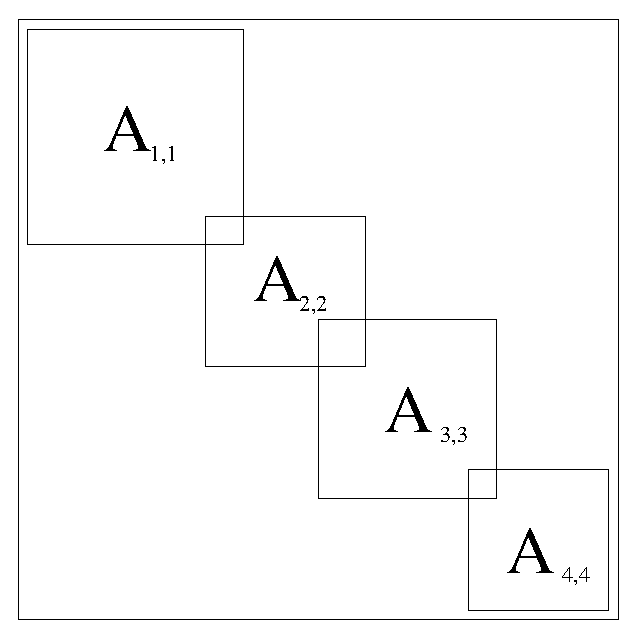
\includegraphics[width=6cm]{bj.eps}
\end{center}
\caption{The block Jacobi matrix with overlapping blocks.}
\label{fig:bj}
\end{figure}

The (damped) block Gauss-Seidel algorithm easily derives from
(\ref{eq:gen_b_jacobi}), by immediately updating the solution vector to
compute the residual. The algorithm is as follows:
\begin{eqnarray}
&& \mbox{On each processor, for each block $i$, Do} \\
&& \label{eq:gen_b_gs}
x^{(k)} = x^{(k-1)} + \omega V_i^T A_{i,i}^{-1} V_i(b - A x^{(k)}).
\end{eqnarray}

%-----------------------------------------------------------------------------
\subsection{Incomplete Factorization Preconditioners}
\label{sec:ilu}
%-----------------------------------------------------------------------------

A broad class of effective preconditioners is based on incomplete
factorization of the linear system matrix.  Such preconditioners are often
referred to as incomplete lower/upper (ILU) preconditioners.  
ILU preconditioning techniques lie between direct and
iterative methods and provide a balance between reliability and
numerical efficiency.  ILU preconditioners are constructed in the factored form
$P=\tilde{L} \tilde{U}$, with $\tilde{L}$ and $\tilde{U}$ being lower
and upper triangular matrices. Solving with $P$ involves two triangular
solutions.

ILU preconditioners are based on the observation
that, although most matrices $A$ admit an LU factorization $A=LU$, where $L$ is
(unit) lower triangular and $U$ is upper triangular, the factors $L$ and $U$ often
contain too many nonzero terms, making the cost of factorization too expensive in
time or memory use, or both.  One type of ILU preconditioner is ILU(0), which 
is defined as proceeding through the standard LU decomposition computations, but keeping 
only those terms in $\tilde{L}$ that correspond to nonzero terms in the lower
triangle of $A$ and similarly keeping only those terms in $\tilde{U}$ that 
correspond to nonzero terms in the upper triangle of $A$.  Although effective, in
some cases the accuracy of the ILU(0) may be insufficient to yield an
adequate rate of convergence. More accurate factorizations will differ
from ILU(0) by allowing some {\em fill-in}. The resulting class of
methods is called ILU($k$), where $k$ is the level-of-fill. A
level-of-fill is attributed to each element that is processed by
Gaussian elimination, and dropping will be based on the level-of-fill.
The level-of-fill should be indicative of the size of the element: the
higher the level-of-fill, the smaller the elements.  

Other strategies consider dropping by value -- for example, dropping
entries smaller than a prescribed threshold. Alternative dropping
techniques can be based on the numerical size of the element to be
discarded. Numerical dropping strategies generally yield more accurate
factorizations with the same amount of fill-in as level-of-fill
methods. The general strategy is to compute an entire row of the
$\tilde{L}$ and $\tilde{U}$ matrices, and then keep only a certain
number of the largest
entries. In this way, the amount of fill-in is
controlled; however, the structure of the resulting matrices is
undefined. These factorizations are usually referred to as ILUT($k$).

When solving a single linear system, ILUT($k$) methods can be more effective
than ILU($k$).  However, in many situations a sequence of linear systems
must be solved where the pattern of the matrix $A$ in each system is
identical but the values of changed.  In these situations, ILU($k$) is 
typically much more effective because the pattern of ILU($k$) will also
be the same for each linear system and the overhead of computing the
pattern is amortized.

%-----------------------------------------------------------------------------
\subsection{Additive Schwarz Preconditioners}
\label{sec:additive}
%-----------------------------------------------------------------------------

\ifpack\ makes very easy to define and use domain decomposition
preconditioners of (overlapping) Schwarz type.

The basic idea of DD methods is to decompose the
computational domain $\Omega$ into $M$ smaller parts $\Omega_i$,
$i=1,\ldots,M$, called subdomains, such that $\cup_{i=1}^{M}
\overline{\Omega_i} = \overline{\Omega}$.  Next, the original problem can
be reformulated within each subdomain $\Omega_i$, of smaller size. This
family of subproblems is coupled one to another through the values of the
unknown solution at subdomain interface. This coupling is then removed at
the expense of introducing an iterative process which involves, at each
step, solutions on the $\Omega_i$ with additional interface conditions on
$\partial \Omega_i \setminus \partial \Omega$.

In overlapping Schwarz preconditioner, the computational domain is
subdivided into {\sl overlapping} subdomains, and local Dirichlet-type
problems are then solved on each subdomain.  The communication between the
solutions on the different subdomains is here guaranteed by the overlapping
region. 

The additive Schwarz preconditioner can be written as:
\begin{equation}
\label{eq:as}
P_{AS}^{-1} = \sum_{i=1}^M P_i A_i^{-1} R_i ,
\end{equation}
where $M$ is the number of subdomains (that is, the number of processors in
the computation), $R_i$ is an operator that restricts the global 
vector to the vector lying on subdomain $\Omega_i$, $P_i$ is an operator that
prolongate from subdomain $\Omega_i$ to $\Omega$, and
\begin{equation}
\label{eq:Ai}
A_i = R_i A P_i.
\end{equation}

\ifpack\ supports two major cases:
\begin{itemize}
\item Minimal-overlap (here referred to as "zero-overlap"): each subdomain
is identified by the set of local rows of the preconditioned matrix;
\item Wider overlap: each subdomain is identified by the set of local rows
of a suitable overlapping matrix.
\end{itemize}
In both cases, each processor is responsible for exactly one subdomain.

In the minimal overlap case, the $R_i$'s and $P_i$'s are not implemented, since the
required components of the residual vector are already local. Besides, matrix
(\ref{eq:Ai}) can be easily extracted from the local matrix, by dropping all
nonzeros corresponding to non-local columns with no 
communications between processors. If a wider overlap
is used, instead, each application of $R_i$ and $P_i$ may require the
importing or exporting of
off-process data, and the construction of (\ref{eq:Ai}) requires
communications.

\smallskip

Once matrices (\ref{eq:Ai}) have been formed, the user still need to define a
strategy to apply the inverse of $A_i$ in (\ref{eq:as}). At this purpose,
any \ifpack\ preconditioner can be adopted. Common choices are:
\begin{itemize}
\item To solve exactly on each subdomain with an complete LU factorization, using the \verb!Ifpack_Amesos!
preconditioner. This is shown in Section~\ref{sec:as_amesos}.
\item To solve using an incomplete LU factorization, as presented in
Section~\ref{sec:as_ilu}.
\item To furtherly decompose the local domain into smaller subdomains,
  then apply a block Jacobi or block Gauss-Seidel preconditioner. This is
  outlined in Section~\ref{sec:as_b_ov}.
\end{itemize}

\begin{remark}
Additive Schwarz preconditioners as reported in equation~(\ref{eq:as}) 
are not scalable: their convergence rate
deteriorates as the number of subdomains (that is, of the processors)
increases. Algebraic techniques
exist to add an algebraic coarse level correction to~(\ref{eq:as}) to make the
preconditioner scalable; 
see for example the documentation of the ML
package~\cite{ml-guide}.
\end{remark}

%-----------------------------------------------------------------------------
\section{General Description of \ifpack\ Preconditioners}
\label{sec:prec}
%-----------------------------------------------------------------------------

All \ifpack\ preconditioners described in this document
are reported in Table~\ref{tab:all_prec}. They are all derived from the 
\verb!Ifpack_Preconditioner!
class.

%\begin{figure}
%\begin{center}
%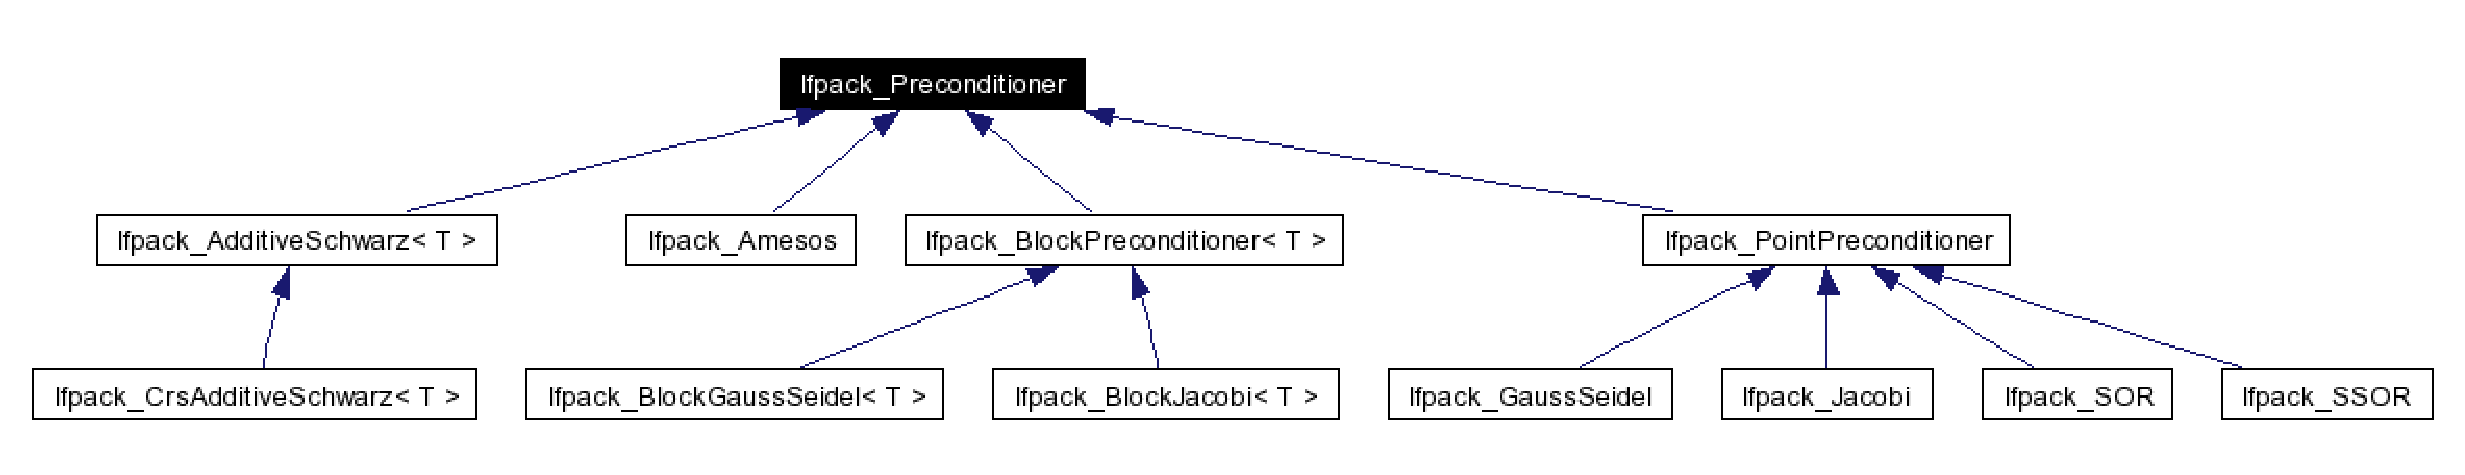
\includegraphics[width=15cm]{Ifpack_Preconditioner.eps}
%\caption{FIXME: UML diagram of  several \ifpack\ preconditioners.}
%\label{fig:if_prec}
%\end{center}
%\end{figure}

\begin{sidewaystable}
\begin{center}
\begin{tabular}{|p{6cm} | c |p{12cm} |}
\hline
Class name & Overlap & Description \\
\hline
\hline
\verb!Ifpack_PointRelaxation!   & 0 & Point (damped) relaxation
preconditioners (Jacobi, Gauss-Seidel, symmetric Gauss-Seidel). Users
can specify the number of Jacobi steps (sweeps), and the damping factor. See
Section~\ref{sec:jacobi} \\
\hline
\verb!Ifpack_BlockRelaxation! & 0 & Block relaxation
preconditioner (Jacobi, Gauss-Seidel, symmetric Gauss-Seidel). Users can store the diagonal blocks as dense or sparse. In the
latter case, any \ifpack\ preconditioner can be used to apply the inverse of
the diagonal block. See Section~\ref{sec:block}. \\
\hline
\verb!Ifpack_AdditiveSchwarz! & user & Generic additive Schwarz
preconditioner. Allows for generic additive Schwarz preconditioners, with
minimal or wider overlap. In the latter case, the user must provide
the overlapping matrix. Any \ifpack\ preconditioner can be used to
solve the local problems. See Section~\ref{sec:additive}. \\
\hline
\verb!Ifpack_IC! & 0 & Incomplete Cholesky factorization, with dropping based
on the level-of-fill of the graph. \\
\hline
\verb!Ifpack_ICT! & 0 & Incomplete Cholesky factorization, with dropping based
on threshold.\\
\hline
\verb!Ifpack_ILU! & 0 & Incomplete LU factorization, with dropping based
on the level-of-fill of the graph. \\
\hline
\verb!Ifpack_ILUT! & 0 & Incomplete LU factorization, with dropping based
on threshold. \\
\hline
\hline
\end{tabular}
\caption{Description of all the \ifpack\ preconditioners reported in this
  document. In the Table, `Overlap' indicates the overlap (with 0 being the
  minimal overlap case, `any' means that the code can construct the
  overlapping matrix for any given positive value).}
\label{tab:all_prec}
\end{center}
\end{sidewaystable}

\verb!Ifpack_Preconditioner! is a pure virtual class, derived from
\verb!Epetra_Operator!, that standarizes the construction and usage of \ifpack\
preconditioners. In fact, all \ifpack\ preconditioners are supposed to behave
as follows:
\begin{enumerate}
\item The object is constructed, passing as only input argument the
pointer of the matrix to be preconditioned, say {\tt A}. {\tt A} has already
been {\tt FillComplete()}'d\footnote{It is supposed that the {\tt OperatorDomainMap()}, {\tt the OperatorRangeMap()}
and
the {\tt RowMatrixRowMap()} of the matrix all coincide, and that each row is ass
igned
to exactly one process..}.
%
\item All the parameters, stored in a \teuchos\ parameters list, are
set using method \verb!SetParameters()!. If \verb!SetParameters()! is not
called, default values will be used.
%
\item The preconditioner is initialized by calling method \verb!Initialize()!.
In this phase, all operations that do not require the matrix values of {\tt A}
are performed (that is, only the structure of {\tt A} is used).
%
\item The preconditioner is constructed by calling method \verb!Compute()!.
In this phase, all the operations that require the matrix values of {\tt A}
are performed
\footnote{For example, in a time dependent setting, if the structure of {\tt
  A} does not change from a given time step to the next but its values do,
  the user can call {\tt Initialize()} only once before the first time step,
  then {\tt Compute()} at each time step.}.
%
\item Method \verb!ApplyInverse()! applies the preconditioner. Any class that
uses \verb!ApplyInverse()! to apply the preconditioner can take advantage of
an \verb!Ifpack_Preconditioner! derived object\footnote{For example, {\tt
  AztecOO} objects can use {\tt Ifpack\_Preconditioner} objects as
    preconditioners.}.
%
\item Method \verb!IsInitialized()! returns {\tt true} is the preconditioner has
been successfully initialized, {\tt false} otherwise.
%
\item Method \verb!IsComputed()! returns {\tt true} is the preconditioner has
been successfully computed, {\tt false} otherwise.
%
\item Method \verb!Condest()! returns an estimation of the condition
number of the preconditioned system.
The condition of a matrix $B$, called $cond_p(B)$, is defined as
$cond_p(B) = \|B\|_p\|B^{-1}\|_p$ in some appropriate norm $p$. 
$cond_p(B)$
gives some indication of how many accurate floating point
digits can be expected from operations involving the matrix and its
inverse.  A condition number approaching the accuracy of a given
floating point number system, about 15 decimal digits in IEEE double
precision, means that any results involving $B$ or $B^{-1}$ may be
meaningless.

The $\infty$-norm of a vector $y$ is defined as the maximum of the
absolute values of the vector entries, and the $\infty$-norm of a
matrix C is defined as
$\|C\|_\infty = \max_{\|y\|_\infty = 1} \|Cy\|_\infty$.
A crude lower bound for the $cond_\infty(C)$ is
$\|C^{-1}e\|_\infty$ where $e = (1, 1, \ldots, 1)^T$.  It is a
lower bound because $cond_\infty(C) = \|C\|_\infty\|C^{-1}\|_\infty
\ge \|C^{-1}\|_\infty \ge |C^{-1}e\|_\infty$. 

More accurate (and expensive) computations for the condition number can be
obtained by calling {\tt Condest(Ifpack\_CG)} or {\tt
  Condest(Ifpack\_GMRES)}\footnote{We note that using CG or GMRES to compute
and estimated condition number is an expensive operations, and should not
be used unless the accurate value of the condition number is required.}.
%
\item Methods \verb!NumInitialize()!, \verb!NumCompute()! and
\verb!NumApplyInverse()! return the number of calls to each phase.
%
\item Methods \verb!InitializeTime()!, \verb!ComputeTime()! and
\verb!ApplyInverseTime()! return the number of CPU-time spent in each phase.
%
\item Methods \verb!InitializeFlops()!, \verb!ComputeFlops()! and
\verb!ApplyInverseFlops()! return the number floating point operations (FLOPS)
  occurred in each phase.
\end{enumerate}


\begin{remark}
Some \ifpack\ preconditioners may require to copy the input \verb!List! object
given in input to \\ \verb!SetParameters()!. In any case, the
user-provided list can go out of scope before \verb!Compute()! is called.
Note that changes to user-provided list after the call to
\verb!SetParameters()! will not affect the preconditioner,
  unless \verb!SetParameters()!  is re-called.
\end{remark}

\begin{remark}
Each \verb!Ipfack_Preconditioner! object overloads the \verb!<<! operator.
Basic information about a given preconditioner can be obtained by simply
using an instruction of the type: \verb!cout << Prec!.
\end{remark}

%-----------------------------------------------------------------------------
\section{The Factory Class}
\label{sec:factory}
%-----------------------------------------------------------------------------

The easiest way to use \ifpack\ is through its factory class. Let us consider
the following fragment of code:
\begin{verbatim}
#include "Ifpack.h"
...
Epetra_RowMatrix* A; // A is already FillComplete()'d
...
Ifpack Factory;
Ifpack_Preconditioner* Prec;
string PrecType = "ILU";
int OverlapLevel = 0;
// create the preconditioner using Create()
Prec = Factory.Create(PrecType, A, OverlapLevel);
assert (Prec != 0);

// specify parameters for ILU
Teuchos::ParameterList List;
List.set("fact: level-of-fill", 5);

Prec->SetParameters();
Prec->Initialize();
Prec->Compute();
...
// Let Problem be an Epetra_LinearProblem
AztecOO Solver(Problem);
Problem.SetPrec(Prec);
// now we can solve with AztecOO
\end{verbatim}

The list of options for {\tt PrecType} is reported in
Table~\ref{tab:factory}. Note that only one word in the above fragment of code
has to be changed to define, for instance, the Gauss-Seidel preconditioner.

\begin{table}
\begin{center}
\begin{tabular}{|p{5cm} | |p{10cm} |}
\hline
{\tt PrecType} & Description \\
\hline
\hline
\tt point relaxation & Point relaxation preconditioner, like Jacobi, Gauss-Seidel,
  and symmetric Gauss-Seidel.\\
\hline
\tt block relaxation & Block relaxation preconditioner, like Jacobi, Gauss-Seidel,
  and symmetric Gauss-Seidel. LAPACK is used to apply the inverse of each
  diagonal block. \\
\hline
\tt block relaxation (Amesos) & Block relaxation preconditioner, like Jacobi, Gauss-Seidel,
  and symmetric Gauss-Seidel. Amesos is used to apply the inverse of each
  block. Requires \ifpack\ support for \amesos. \\
\hline
\tt IC & Incomplete Cholesky factorization on each subdomain. \\
\hline
\tt ICT & Incomplete Cholesky factorization with threshold on each subdomain. \\
\hline
\tt ILU & Incomplete LU factorization on each subdomain. \\
\hline
\tt ILUT & Incomplete LU with threshold on each subdomain. \\
\hline
\tt Amesos & Complete LU factorization on each subdomain. Requires \ifpack\
  support for \amesos. \\
\hline
\end{tabular}
\end{center}
\caption{List preconditioners supported by the Factory class.}
\label{tab:factory}
\end{table}

%-----------------------------------------------------------------------------
\section{Examples of Usage}
\label{sec:usage}
%-----------------------------------------------------------------------------

This section contains several examples of usage of \ifpack\ preconditioners. A
detailed list of \ifpack\ parameters is reported in
section~\ref{sec:parameters}.

%-----------------------------------------------------------------------------
\subsection{Point Preconditioners}
\label{sec:point_ex}
%-----------------------------------------------------------------------------

An example of usage of point relaxation preconditioners (in this case, Gauss-Seidel) is as
follows:
\begin{verbatim}
#include "Teuchos_ParameterList.hpp"
#include "Ifpack_PointRelaxation.h"
\end{verbatim}
Let \verb!A! be a pointer to an \verb!Epetra_RowMatrix! derived object,
  and let \verb!Problem! be a pointer to an \verb!Epetra_LinearProblem!.
We suppose that \verb!A! and 
\verb!Problem! are properly set, and
method \verb~FillComplete()~ has been called. At this point, we can create the
preconditioner as
\begin{verbatim}
Teuchos::ParameterList List;
List.set("relaxation: type", "Gauss-Seidel");

Ifpack_PointRelaxation Prec(A);

IFPACK_CHK_ERR(Prec.SetParameters(List));
IFPACK_CHK_ERR(Prec.Initialize());
IFPACK_CHK_ERR(Prec.Compute());
\end{verbatim}
Now, we can set the IFPACK preconditioner for AztecOO:
\begin{verbatim}
AztecOO AztecOOProblem(Problem);
AztecOOProblem.SetPrecOperator(Prec);
\end{verbatim}
as call \verb!AztecOO.Iterate()! as required.

Macro \verb!IFPACK_CHK_ERR()! can be used to check return values. If the
return value if different from 0, the macro prints out a warning message on
\verb!cerr!, and returns.

%-----------------------------------------------------------------------------
\subsection{Block Preconditioners}
\label{sec:block_ex}
%-----------------------------------------------------------------------------

From the point of view of the implementation block preconditioner
are sensibly more complex than their point counterpart:
\begin{enumerate}
\item A strategy to define the blocks has to be chosen (for instance, 
a linear partitioner, or a graph decomposition algortithm);
\item block Jacobi and block Gauss-Seidel algorithms require the application
of the inverse of each diagonal block $A_{i,i}$. Blocks of small dimension
should be stored as dense matrices, while larger blocks require sparse
storage. In this latter case, to apply the inverse of the block can be
reformulated as applying a preconditioner for matrix
$A_{i,i}$.
The code must allow for different choices of block preconditioners.
\end{enumerate}

\smallskip

Let us start with the definition of the blocks. 
\ifpack\ provides the following options:
\begin{itemize}
\item a linear partitioning, using class \verb!Ifpack_LinearPartitioner!;
\item a simple greedy algorithm, using class \verb!Ipfack_GreedyPartitioner!;
\item an interface to METIS, using class \verb!Ifpack_METISPartitioner!.
\end{itemize}
It is important to note that all blocks are {\sl local} -- that is, 
  all partitioner schemes will {\sl always} decompose the local graph 
  only\footnote{If used in conjuction with class {\tt Ifpack\_AdditiveSchwarz},
    blocks can span more than one processor.}.

All \ifpack\ partitioners are derived from the pure virtual class
\verb!Ifpack_Partitioner!, and all require in the constructor phase
an \verb!Ifpack_Graph! object. \verb!Ifpack_Graph!'s can be easily
created (as light-weigth) conversions from \verb!Epetra_RowMatrix!'s
and \verb!Epetra_CrsGraph!'s, as follows At this point, we can create the
preconditioner as
\begin{verbatim}
#include "Ifpack_Graph.h"
#include "Ifpack_Graph_Epetra_CrsGraph.h"
#include "Ifpack_Graph_Epetra_RowMatrix.h"

// use either CsrA or RowA, depending on your application
Epetra_CrsMatrix* CrsA;
Epetra_RowMatrix* RowA;

Ifpack_Graph CrsGraph* CrsGraph =
  new Ifpack_Graph_CrsGraph(&(CrsA->Graph()));

Ifpack_Graph RowGrap* RowGraph  =
  new Ifpack_Graph_RowMatrix(RowA);
\end{verbatim}
Note that the \verb!Partitioner! object will decompose the graph (either
\verb!CrsGraph! or \verb!RowGraph!) into
non-overlapping sets (that is, each graph vertex is assigned to exactly one
set).

The following fragment of code shows how to use a greedy partitioner to define
4 local blocks for a given \verb!Ifpack_Graph!.

\begin{verbatim}
#include "Ifpack_Graph.h"
#include "Ifpack_GreedyPartitioner.h"
#include "Ifpack_BlockRelaxation.h"
#include "Teuchos_ParameterList.hpp"
...

Ifpack_Graph* Graph;   
// Graph is created here

Teuchos::ParameterList List;
List.set("partitioner: local parts", 4);
Ifpack_Partitioner* Partitioner = new Ifpack_GreedyPartitioner(Graph);

// set the parameters (in this case the # of blocks only)
Partitioner->SetParameters(List);

// compute the partition
Partitioner->Compute();
\end{verbatim}

Once an \verb!Ifpack_Partitioner! is created, we are ready to
compute the block preconditioner. This requires the extraction of
all the diagonal bocks of equation (\ref{eq:D}). In \ifpack, the
user can choose to store the $A_{i,i}$ as dense matrices, or a sparse
matrices. In the former case, the inverse of each block is applied using
LAPACK\footnote{LAPACK is used to factorize the matrix, then each application
  of $A_{i,i}^{-1}$ results in a dense linear system solution.}. In the
  latter, the user can specify any valid \verb!Ifpack_Preconditioner!.

As an example, we now create a block Jacobi preconditioner for 
a given \verb!Epetra_RowMatrix!, say \verb!A!,
with damping parameter of 0.67, and 2 sweeps. Each diagonal block is stored as a dense
matrix.

\begin{verbatim}
#include "Ifpack_BlockRelaxation.h"
#include "Ifpack_DenseContainer.h"
...

Ifpack_Partitioner* Partitioner;
// Partitioner is created here

Ifpack_Preconditioner* Prec =
  new Ifpack_BlockRelaxation<Ifpack_DenseContainer>(A);

Teuchos::ParameterList List;
List.set("relaxation: sweeps", 2);
List.set("relaxation: damping parameter", 0.67);
Prec->SetParameters(List);
Prec->Compute();
\end{verbatim}
The previous example makes use of a dense containers to store
the diagonal blocks.
In \ifpack, a {\sl container} is an object that contains all the necessary
data to solve the linear system with any given $A_{i,i}$. 
\verb!Ifpack_DenseContainer! stores each $A_{i,i}$ as
\verb!Epetra_SerialDenseMatrix!. Alternatively, one can use 
\verb!Ipfack_SparseContainer! to store each block as an
\verb!Epetra_CrsMatrix!. Sparse containers are templated with an
\verb!Ifpack_Preconditioner!, so that the user can specify which \ifpack\
  preconditioner has to be used to apply the inverse of each sparse block.

The following fragment of code illustrates how to use the direct factorization
of Amesos (through class \verb!Ifpack_Amesos!\footnote{This requires \ifpack\
	   to be configured with option {\tt --enable-amesos}.}) with sparse containers. The preconditioner will be a block Gauss-Seidel one.

\begin{verbatim}
#include "Ifpack_BlockRelaxation.h"
#include "Ifpack_SparseContainer.h"
#include "Ifpack_Amesos.h"
...

Ifpack_Partitioner* Partitioner;
// Partitioner is created here

Ifpack_Preconditioner* Prec =
  new Ifpack_BlockRelaxation<Ifpack_SparseContainer<Ifpack_Amesos> >(A);

Teuchos::ParameterList List;
List.set("relaxation: sweeps", 2);
List.set("amesos: solver type", "Amesos_Klu");
Prec->SetParameters(List);
Prec->Initialize();
Prec->Compute();
\end{verbatim}

Option \verb!amesos: solver type! specifies the \amesos\ solver that
has to be adopted. If the selected solver is not available, then
\verb!Ifpack_Amesos! will create an \verb!Amesos_Klu! solver\footnote{KLU is
  compiled by default with \amesos. Please consult the \amesos\ documentation
    for more details.}.
As {\sl any} \ifpack\ preconditioner can be used, one can also adopt, for
instance, a point Gauss-Seidel algorithm in each block:
\begin{verbatim}
Ifpack_Preconditioner* Prec =
  new Ifpack_BlockRelaxation<Ifpack_SparseContainer<Ifpack_GaussSeidel> >(A);
\end{verbatim}

A call to \verb!SetParameters(List)! will set the parameters for the block
preconditioner.

%-----------------------------------------------------------------------------
\subsection{Additive Schwarz with Exact Local Solves}
\label{sec:as_amesos}
%-----------------------------------------------------------------------------

The following fragment of code shows the use of additive preconditioners. The
local subproblems with matrix $A_i$ are solved using a (complete) LU
factorization through \amesos.
\begin{verbatim}
#include "Ifpack_AdditiveSchwarz.h"
#include "Ifpack_Amesos.h"

Epetra_RowMatrix* A;
// Here the elements of A are filled, and FillComplete() is called.

int OverlapLevel = 0;
Ifpack_Preconditioner* Prec = 
  new Ifpack_AdditiveSchwarz<Ifpack_Amesos>(A, OverlapLevel);

Teuchos::ParameterList List;
IFPACK_CHK_ERR(Prec->SetParameters(List));
IFPACK_CHK_ERR(Prec->Initialize());
IFPACK_CHK_ERR(Prec->Compute());
\end{verbatim}

\begin{remark}
Complete factorizations can be expensive to compute, especially for problems
arising from discretizations on 3D grids. The user should consider complete
factorizations if the local problems are small, or when other, cheaper
preconditioners fail.
\end{remark}

%-----------------------------------------------------------------------------
\subsection{Additive Schwarz with ILU}
\label{sec:as_ilu}
%-----------------------------------------------------------------------------

The following fragment of code shows the use of additive preconditioners. The
local subproblems with matrix $A_i$ are solved using an incomplete
factorization.
\begin{verbatim}
#include "Ifpack_AdditiveSchwarz.h"
#include "Ifpack_ILU.h"

Epetra_RowMatrix* A;
// Here the elements of A are filled, and FillComplete() is called.

int OverlapLevel = 0;
Ifpack_Preconditioner* Prec = 
  new Ifpack_AdditiveSchwarz<Ifpack_ILU>(A, OverlapLevel);

Teuchos::ParameterList List;
List.set("fact: level of fill", 2);
IFPACK_CHK_ERR(Prec->SetParameters(List));
IFPACK_CHK_ERR(Prec->Initialize());
IFPACK_CHK_ERR(Prec->Compute());
\end{verbatim}

The difficulty with this type of preconditioner is that it tends to become
less robust and require more iterations as the number of processors used
increases.  This effect can be offset to some extent by allowing {\em
overlap}.  Overlap refers to having processors redundantly own certain rows
of the matrix for the ILU factorization.  Level-1 overlap is defined so
that a processor will include rows that are part of its original set.  In
addition, if row $i$ is part of its original set and row $i$ of $A$ has a
nonzero entry in column $j$, then row $j$ will also be included in the
factorization on that processor.  Other levels of overlap are computed
recursively.  IFPACK supports an arbitrary level of overlap.  However,
level-1 is often most effective.  Seldom more than 3 levels are needed. 

\smallskip

The user can access the factorization of the local matrix produced by
templating \verb!Ifpack_AdditiveSchwarz! with classes \verb!Ifpack_IC!,
  \verb!Ifpack_ICT!, \verb!Ifpack_ILU! and \verb!Ifpack_ILUT! in the following
  way:
\begin{verbatim}
Ifpack_Preconditioner* Prec = 
  new Ifpack_AdditiveSchwarz<Ifpack_ILU>(A, OverlapLevel);

Ifpack_ILU* Inverse = Prec->Inverse();
\end{verbatim}
Then, the total number of nonzeros in the L and U factors can be queried as
follows:
\begin{verbatim}
int NumGlobalNonzerosLU = Inverse->NumGlobalNonzeros();
\end{verbatim}
The L and U factors are stored as \verb!Epetra_CrsMatrix!'s, whose pointers
can be obtained as follows\footnote{For classes {\tt Ifpack\_IC} and {\tt
  Ifpack\_ICT} the user shall use method {\tt H()}.}:
\begin{verbatim}
const Epetra_CrsMatrix& L = Inverse->L();
const Epetra_CrsMatrix& U = Inverse->U();
\end{verbatim}

%-----------------------------------------------------------------------------
\subsection{Additive Schwarz with Local Block Preconditioners}
\label{sec:as_b_ov}
%-----------------------------------------------------------------------------

Another possible technique to apply the inverse of $A_i$ in (\ref{eq:as})
is to adopt a block preconditioner, like block Jacobi 
or block Gauss-Seidel (see
Section~\ref{sec:block}). This requires a
bit more work, as we have to specify the partitioner, and the container. Let
us start with dense containers.

The required include files are:
\begin{verbatim}
#include "Ifpack_AdditiveSchwarz.h"
#include "Ifpack_BlockPreconditioner.h"
#include "Ifpack_Graph_Epetra_RowMatrix.h"
#include "Ifpack_DenseContainer.h"
\end{verbatim}

Let \verb!A! be an \verb!Epetra_RowMatrix!. We suppose that
\verb!FillComplete()! has been called. 

As always, we create a parameters list, that will be used
for all \ifpack\ objects:
\begin{verbatim}
Teuchos::ParameterList List;
\end{verbatim}
At this point we can create the block Jacobi preconditioner as follows:
\begin{verbatim}
Ifpack_Preconditioner* Prec = 
  new Ifpack_AdditiveSchwarz<
    Ifpack_BlockPreconditioner<Ifpack_DenseContainer> >(A);

Prec->SetParameters(List);
Prec->Initialize();
Prec->Compute();
\end{verbatim}
As we have used {\tt Ifpack\_DenseContainer}, blocks are stored are dense
matrices, and LAPACK is used to apply the inverse of each block. This can be a
limiting factor for large blocks. In this latter case, it is preferable to
store the blocks are sparse matrices, and use a sparse solver to apply their
inverse. This can be done by resorting to {\tt Ifpack\_SparseContainer}. 
Sparse containers can be used with minor modifications. The only difference is
that we also have to specify how to apply the inverse of each block, for
instance using the exact factorizations of \amesos:
\begin{verbatim}
Ifpack_Preconditioner* Prec = 
  new Ifpack_AdditiveSchwarz<Ifpack_BlockPreconditioner
    <Ifpack_SparseContainer<Ifpack_Amesos> > >(A);
\end{verbatim}

Should the user want to use a block Gauss-Seidel preconditioner (where each
block is defined by partitioning the local graph of the overlapping matrix),
he/she could proceed as follows:
\begin{verbatim}
Teuchos::ParameterList List;
List.set("relaxation: damping factor", .67);
List.set("relaxation: sweeps",5);
List.set("partitioner: local parts", 4);
List.set("partitioner: overlap", OverlapLevel);

Epetra_RowMatrix* A; // A is FillComplete()'d.

Ifpack_Preconditioner* Prec =
  new Ifpack_AdditiveSchwarz<Ifpack_BlockPreconditioner
      <Ifpack_SparseContainer<Ifpack_Amesos> > >(A,OverlapLevel);

IFPACK_CHK_ERR(Prec->SetParameters(List));
IFPACK_CHK_ERR(Prec->Compute());
\end{verbatim}

%-----------------------------------------------------------------------------
\section{Parameters for \ifpack\ preconditioners}
\label{sec:parameters}
%-----------------------------------------------------------------------------

The parameters that affect the \ifpack\ preconditioners are reported
below. It is important to note that parameters for all \ifpack\
preconditioners must be spelled as indicated:
misspelled parameters will be ignored, parameters are case sensitive, and words
  are separated by one space only.

\smallskip

For more details about the \teuchos\ parameters list we refer to the
\teuchos\ documentation.  Table~\ref{tab:teuchos} briefly reports the most
important methods of this class.
\ifpack\ requires just a very basic usage of the parameters list.
Input parameters are set via method \verb!set(Name,Value)!, where
\verb!Name! is a string containing the parameter name, and \verb!Value! is the
specified parameter value, whose type can be any C++ object or pointer. 

\begin{table}[htbp]
  \centering
  \begin{tabular}{| p{4cm} | p{10cm} |}
    \hline
    \verb!set(Name,Value)! & Add entry \verb!Name! with value and type
    specified by \verb!Value!. Any C++ type (like int, double, a
    pointer, etc.) is valid. \\
    \verb!get(Name,DefValue)! & Get value (whose type is automatically
    specified by \verb!DefValue!). If not present, return
    \verb!DefValue!. \\
    \verb!subList(Name)! & Get a reference to sublist \verb!List!. If not
    present, create the sublist. \\
    \hline
  \end{tabular}
  \caption{Some methods of Teuchos::ParameterList class.}
  \label{tab:teuchos}
\end{table}

\smallskip

\choicebox{\tt relaxation: type}{[{\tt string}] Relaxation scheme. Valid
  choices are: {\tt Jacobi}, {\tt Gauss-Seidel}, {\tt symmmetric
    Gauss-Seidel}. Default: {\tt Jacobi}.}

\choicebox{\tt relaxation: sweeps}{[{\tt int}] Number of sweeps of
  the point relaxation preconditioner. Default: {\tt 1}.}

\choicebox{\tt relaxation: damping factor}{[{\tt double}] This is the value for $\omega$ 
  in formulae (\ref{eq:jacobi}), (\ref{eq:gs}), (\ref{eq:sor}) and
    (\ref{eq:ssor}). Default: {\tt 1.0}.}
				 
\choicebox{\tt relaxation: min diagonal value}{[{\tt double}] Replace diagonal
  values whose absolute value is less than the specified value by this value
    (for point relaxation methods only). Default: {\tt 1e-9}.}

\choicebox{\tt relaxation: zero starting solution}{[{\tt bool}] 
  If {\tt true}, the input values in the preconditioned vector will be used as
    starting solution (for relaxation methods only).  Default: {\tt true}.}

\choicebox{\tt partitioner: type}{[{\tt string}] Defines how to build the
  local blocks (for block relaxation methods). Valid choices are:
  {\tt linear} (use a simple linear decomposition), {\tt greedy} 
  (use a greedy algorithm to partition the local graph), 
  or {\tt METIS} (call METIS on the local graph). Default: {\tt linear}.}

\choicebox{\tt partitioner: local parts}{[{\tt int}] Number of (local)
  subgraphs (for block relaxation methods only). Default: 4.}

\choicebox{\tt partitioner: overlap}{[{\tt int}] Overlap among blocks. Only
  for block Jacobi methods. Default: 0.}

\choicebox{\tt partitioner: root node}{[{\tt int}] Root node, for greedy
  algorithm only. Default: 0}

\choicebox{\tt schwarz: combine mode}{[{\tt Epetra\_CombineMode}].
Default: {\tt Zero}.
It can assume one of the following values:
{\tt Add}: Components on the receiving processor will be added together;
{\tt Zero}: Off-processor components will be ignored;
{\tt Insert}: Off-processor components will be inserted into locations on
receiving processor replacing existing values.
{\tt Average}: Off-processor components will be averaged with existing;
{\tt AbsMax}: Magnitudes of Off-processor components will be
maxed with magnitudes of existing components on the receiving
processor. Note that, for non-zero overlap values, the preconditioner is in general
  non-symmetric, due to the handling of the overlapping region. Set this parameter to {\tt Insert} if a
    symmetric preconditioner is required.}

\choicebox{\tt amesos: solver type}{[{\tt string}]. Defines the Amesos solver to be
  used by class Ifpack\_Amesos. Valid values are:
{\tt Amesos\_Lapack},
{\tt Amesos\_Klu},
{\tt Amesos\_Umfpack},
{\tt Amesos\_Superlu},
{\tt Amesos\_Mumps},
{\tt Amesos\_Dscpack}. Default: {\tt Amesos\_Klu} Default: {\tt Amesos\_Klu}.}

\choicebox{\tt fact: level-of-fill}{[{\tt int}] Level-of-fill for IC and ILU.}

\choicebox{\tt fact: ict level-of-fill}{[{\tt double}] Level-of-fill for ICT.}

\choicebox{\tt fact: ilut level-of-fill}{[{\tt double}] Level-of-fill for
  ILUT.}

\choicebox{\tt fact: relax value}{[{\tt double}] Relaxation value.}

\smallskip

It is often convenient to compute the incomplete factorization of a given
matrix, say $A$, by ``filtering'' this matrix, so that it behaves ``well''
during the factorization process. The idea to filter the matrix is very
simple: instead of using matrix $A$, we perform the factorization  on 
a modified matrix $B$\footnote{This matrix is never built. The code modifies
  the {\tt ExtractMyRowCopy()} method, and updated the diagonal value.}, whose elements are defined as
\begin{equation}
\label{eq:B}
\begin{array}{lcr}
B_{i,j} = A_{i,j} \quad \quad i \neq j \\
B_{i,i} = \alpha \; \; sgn(A_{i,i}) + \rho A_{i,i},
  \end{array}
\end{equation}
where $\alpha$ and $\rho$ are two real parameters, to be determined by the
user. $\alpha$ represents and absolute threshold added to the matrix, while
$\rho$ is a relative threshold (that is, the actual diagonal value of the matrix to
be factored is $\rho$ times the original value). 

\smallskip

\choicebox{\tt fact: absolute threshold}{[{\tt double}] Value $\alpha$ in equation (\ref{eq:B}). }

\choicebox{\tt fact: relative threshold}{[{\tt double}] Value $\rho$ in
  equation (\ref{eq:B}). }


%-----------------------------------------------------------------------------
\section{Analysis Tools}
\label{sec:analysis}
%-----------------------------------------------------------------------------

\ifpack\ contains the following tools to analyze a linear system matrix:
\begin{itemize}
\item Function {\tt Ifpack\_Analyze()} reports some information about the
structure of the matrix, its diagonal elements, and others.
\item Function {\tt Ifpack\_PrintSparsity()} prints on a PostScript file the
sparsity pattern of a given {\tt Epetra\_RowMatrix}.
\item Function {\tt Ifpack\_PrintSparsitySimple()}, to be used only with small
matrices, prints on a screen the
sparsity pattern of a given {\tt Epetra\_RowMatrix}.
\end{itemize}

%-----------------------------------------------------------------------------
%-----------------------------------------------------------------------------
\section{Configuring and Building \ifpack}
\label{sec:config}
%-----------------------------------------------------------------------------

We recommend to configure and build \ifpack\ as part of the standard 
\trilinos~build and configure process.  In fact,
\ifpack\ is built by default if you follow the standard \trilinos~configure
and build directions. Please refer to the \trilinos~documentation 
for information about the configuration and building of
other \trilinos~packages.

\smallskip

To configure and build \ifpack\ through \trilinos, you may need do the
following (actual configuration options may vary depending on the
specific architecture, installation, and user's need).  It's assumed
that shell variable \verb!$TRILINOS_HOME!  identifies the
\trilinos~directory, and, for example, that we are compiling under LINUX
and MPI.
\begin{verbatim}
% cd $TRILINOS_HOME
% mkdir LINUX_MPI
% cd LINUX_MPI
% $TRILINOS_HOME/configure  --with-mpi-compilers \
    --prefix=$TRILINOS_HOME/LINUX_MPI
% make
% make install
\end{verbatim}

\ifpack\ is configured and built using the GNU autoconf~\cite{Autoconf} and
automake~\cite{Automake} tools. 
\ifpack configuration and compilation can be tuned by several flags.
The user may type 
\begin{verbatim}
% configure --help
\end{verbatim}
in the \ifpack\ source directory for a complete list. Here, we briefly report
the list of packages (included or not in Trilinos) that are supported 
by \ifpack:

\medskip

\choicebox{\tt --enable-amesos}
{Enables support for the \amesos~package, which can be used to solve the
  local subproblems in Schwarz-type preconditioners, or in
    block Jacobi and block Gauss-Seidel preconditioners.}

\choicebox{\tt --enable-aztecoo}
{Enable support for the \aztecoo\ package. \aztecoo~is used in several tests
  and examples.}

\choicebox{\tt --enable-teuchos}
{Enable support for the \teuchos\ package, whose parameters list is used by
  several \ifpack\ classes.}

\choicebox{\tt --enable-triutils}
{Enable support for the \triutils\ package, which is used in some examples and
  test to generate the linear system.}

\choicebox{\tt --enable-ifpack-metis}
{Enable support for the \metis\ package, version 4.0 or later. \metis\ can be
  used to create block preconditioners.}

\begin{remark}
\ifpack\ cannot be compiled without the \epetra\ library.
\end{remark}


\clearpage
\newpage
%@HEADER
% ************************************************************************
% 
%          Trilinos: An Object-Oriented Solver Framework
%              Copyright (2001) Sandia Corporation
% 
% Under terms of Contract DE-AC04-94AL85000, there is a non-exclusive
% license for use of this work by or on behalf of the U.S. Government.
% 
% This program is free software; you can redistribute it and/or modify
% it under the terms of the GNU General Public License as published by
% the Free Software Foundation; either version 2, or (at your option)
% any later version.
%   
% This program is distributed in the hope that it will be useful, but
% WITHOUT ANY WARRANTY; without even the implied warranty of
% MERCHANTABILITY or FITNESS FOR A PARTICULAR PURPOSE.  See the GNU
% General Public License for more details.
%   
% You should have received a copy of the GNU General Public License
% along with this program; if not, write to the Free Software
% Foundation, Inc., 675 Mass Ave, Cambridge, MA 02139, USA.
% 
% Questions? Contact Michael A. Heroux (maherou@sandia.gov)
% 
% ************************************************************************
%@HEADER

\section{The Teuchos Utility Classes}
\label{chap:teuchos}

Teuchos (pronounced ``te-fos'') is a collection of portable C++ tools
that facilitate the development of scientific codes.  Only a few of the many
tools in Teuchos are mentioned in this section.
For more details on all of the capabilities provided by Teuchos, please 
refer to the online documentation (\verb!http://software.sandia.gov/trilinos/packages/teuchos!).

Teuchos classes have been divided between a``standard'' build and an
``extended'' build. The ``standard'' build contains the general purpose
templated tools like BLAS/LAPACK wrappers, parameter lists, a command-line parser,
serial dense matrices, timers, flop counters, and a reference-counted pointer class.  
These tools are built by default when Teuchos is enabled using the 
configure option \verb!--enable-teuchos!. 
The ``extended'' build contains more special purpose tools like 
XML parsing and MPI communicators, which can be included in the Teuchos
library by using the configure option \verb!--enable-teuchos-extended!.

\medskip

In this Chapter, we will present the following ``standard'' build classes:
\begin{itemize}

\item \verb!Teuchos::ScalarTraits! class (Section~\ref{sec:teuchos:ScalarTraits}):
  The ScalarTraits class provides a basic interface to scalar types (float, double, 
  complex$<$float$>$, complex$<$double$>$) that is used by the templated computational
  classes within Teuchos.  It is the mechanism by which Teuchos' capabilities 
  can be extended to support arbitrary precisions.

\item \verb!Teuchos::SerialDenseMatrix! class (Section~\ref{sec:teuchos:SDM}): 
  The SerialDenseMatrix is a templated version of the \verb!Epetra_SerialDenseMatrix! class
  that is most often used to interface with the templated BLAS/LAPACK wrappers.

\item \verb!Teuchos::BLAS! class (Section~\ref{sec:teuchos:BLAS}):
  The BLAS class provides templated wrappers
  for the native BLAS library and can be extended to provide arbitrary precision
  computations.  

\item \verb!Teuchos::LAPACK! class (Section~\ref{sec:teuchos:LAPACK}):
  The LAPACK class provides templated wrappers for the native LAPACK library.

\item \verb!Teuchos::ParameterList! class (Section~\ref{sec:teuchos:ParameterList}):
  ParameterList is a container that can be used to group all the parameters required by a
  given piece of code.

\item \verb!Teuchos::RefCountPtr! class (Section~\ref{sec:teuchos:RefCountPtr}):
  RefCountPtr is a smart reference-counted pointer class, which provides a functionality
  similar to the garbage collector of Java. 

\item \verb!Teuchos::TimeMonitor! class (Section~\ref{sec:teuchos:TimeMonitor}):
  TimeMonitor is a timing class that starts a timer when it is initialized and
  stops it when the destructor is called on the class.

\item \verb!Teuchos::CommandLineProcessor! class (Section~\ref{sec:teuchos:CLP}): 
  CommandLineProcessor is a class that helps parse command line input arguments from 
  \verb!(argc,argv[])!.   
\end{itemize}

%%%
%%%
%%%

\subsection{Teuchos::ScalarTraits}
\label{sec:teuchos:ScalarTraits}

The ScalarTraits class provides a basic interface to scalar types (float, double, 
complex$<$float$>$, complex$<$double$>$) that is used by the templated 
computational classes within Teuchos.  This interface includes a definition of
the magnitude type and methods for obtaining random numbers, representations of 
zero and one, the square root, and machine-specific parameters.  
The Teuchos classes that utilize this scalar traits mechanism are 
\verb!Teuchos::SerialDenseMatrix!, \verb!Teuchos::BLAS!, and \verb!Teuchos::LAPACK!.  

ScalarTraits enables the extension of Teuchos' computational
capabilities to any scalar type that can support its basic interface.  In particular, 
this interface can be used for arbitrary precision scalar types.  An interface to the
arbitrary precision library ARPREC \cite{arprec:02} is available if Teuchos
is configured with \verb!--enable-teuchos-arprec!. Teuchos must also be configured
with the local ARPREC library paths (\verb!--with-libs!, \verb!--with-incdirs!, and 
\verb!--with-libdirs!).  To obtain more information on ARPREC or download the 
source code, see {\tt http://crd.lbl.gov/$\sim$dhbailey/mpdist/}.

\begin{remark} To enable complex arithmetic (complex$<$float$>$ or complex$<$double$>$) 
support in ScalarTraits or any dependent classes, configure Teuchos with {\tt --enable-teuchos-complex}.
\end{remark}

%%%
%%%
%%%

\subsection{Teuchos::SerialDenseMatrix}
\label{sec:teuchos:SDM}

\verb!Teuchos::SerialDenseMatrix! is a templated version of the SerialDenseMatrix class in \verb!Epetra!
(Chapter \ref{chap:epetra_mat}).  It is most useful for interfacing with the templated BLAS and 
LAPACK wrappers, which will be discussed in Sections \ref{sec:teuchos:BLAS} and \ref{sec:teuchos:LAPACK}.  
However, by enabling the simple construction and manipulation of small dense matrices, 
the SerialDenseMatrix class has also been used as an independent tool in many 
Trilinos packages.

\verb!Teuchos::SerialDenseMatrix! provides a serial interface to a small dense matrix
of templated scalar type.  This means a SerialDenseMatrix object can be created for any scalar type 
supported by Teuchos::ScalarTraits (Section \ref{sec:teuchos:ScalarTraits}).  To use the 
Teuchos::SerialDenseMatrix class, include the header:

{\small 
\begin{verbatim}
#include "Teuchos_SerialDenseMatrix.hpp"
\end{verbatim}}
Creating a double-precision matrix can be done in several ways:
{\small 
\begin{verbatim}
// Create an empty matrix with no dimension
Teuchos::SerialDenseMatrix<int,double> Empty_Matrix;
// Create an empty 3x4 matrix
Teuchos::SerialDenseMatrix<int,double> My_Matrix( 3, 4 );
// Basic copy of My_Matrix
Teuchos::SerialDenseMatrix<int,double> My_Copy1( My_Matrix ),
// (Deep) Copy of principle 3x3 submatrix of My_Matrix
                  My_Copy2( Teuchos::Copy, My_Matrix, 3, 3 ),
// (Shallow) Copy of 2x3 submatrix of My_Matrix
                  My_Copy3( Teuchos::View, My_Matrix, 3, 4, 1, 1 );
\end{verbatim}}
The matrix dimensions and strided storage information can be obtained:
{\small
\begin{verbatim}
int rows = My_Copy3.numRows();  // number of rows
int cols = My_Copy3.numCols();  // number of columns
int stride = My_Copy3.stride(); // storage stride
\end{verbatim}}
Matrices can change dimension:
{\small
\begin{verbatim}
Empty_Matrix.size( 3, 3 );      // size non-dimensional matrices
My_Matrix.resize( 3, 3 );       // resize matrices and save values
\end{verbatim}}
Filling matrices with numbers can be done in several ways:
{\small 
\begin{verbatim}
My_Matrix.random();             // random numbers
My_Copy1.putScalar( 1.0 );      // every entry is 1.0
My_Copy2(1,1) = 10.0;           // individual element access
Empty_Matrix = My_Matrix;       // copy My_Matrix to Empty_Matrix 
\end{verbatim}}
Basic matrix arithmetic can be performed:
{\small
\begin{verbatim}
Teuchos::SerialDenseMatrix<int,double> My_Prod( 3, 2 );
// Matrix multiplication ( My_Prod = 1.0*My_Matrix*My_Copy^T )
My_Prod.multiply( Teuchos::NO_TRANS, Teuchos::TRANS, 
                  1.0, My_Matrix, 1.0, My_Copy3, 0.0 );
My_Copy2 += My_Matrix;         // Matrix addition
My_Copy2.scale( 0.5 );         // Matrix scaling
\end{verbatim}}
The pointer to the array of matrix values can be obtained:
{\small
\begin{verbatim}
double* My_Array = My_Matrix.values();   // pointer to matrix values
double* My_Column = My_Matrix[2];        // pointer to third column values
\end{verbatim}}
The norm of a matrix can be computed:
{\small
\begin{verbatim}
double norm_one = My_Array.normOne();        // one norm
double norm_inf = My_Array.normInf();        // infinity norm
double norm_fro = My_Array.normFrobenius();  // frobenius norm
\end{verbatim}}
Matrices can be compared:
{\small
\begin{verbatim}
// Check if the matrices are equal in dimension and values
if (Empty_Matrix == My_Matrix) {
  cout<< "The matrices are the same!" <<endl;
}
// Check if the matrices are different in dimension or values
if (My_Copy2 != My_Matrix) {
  cout<< "The matrices are different!" <<endl;
}
\end{verbatim}}
A matrix can be sent to the output stream:
{\small
\begin{verbatim}
cout<< My_Matrix << endl;
\end{verbatim}}
This section presents examples of all the methods in the 
{\tt Teuchos::SerialDenseMatrix} class and can be found in
\TriExe{teuchos/ex1.cpp}.  There is also a specialization of
this class for serial dense vectors that includes additional creation, accessor, 
arithmetic, and norm methods ({\tt Teuchos::SerialDenseVector}).

%%%
%%%
%%%

\subsection{Teuchos::BLAS}
\label{sec:teuchos:BLAS}

The \verb!Teuchos::BLAS! class provides templated wrappers for the native BLAS library.
This class has been written to facilitate the interface between C++ codes and BLAS,
which are written in Fortran.  Unfortunately, the interface between C++ and Fortran
function calls is not standard across all computer platforms.  The \verb!Teuchos::BLAS!
class provides C++ wrappers the BLAS kernels that are specialized during the Teuchos
configuration.  This insulates the rest of Teuchos and its users from the details of
the Fortran to C++ translation.

The \verb!Teuchos::BLAS! provides these C++ wrappers for a substantial subset of the 
BLAS kernels (Figure \ref{blas_kernels}).
The native BLAS library implementations of those kernels
will be used for the standard scalar types (float, double, complex$<$float$>$, complex$<$double$>$).  
However, \verb!Teuchos::BLAS! also has a
templated version of each of these kernels.  Paired with \verb!Teuchos::ScalarTraits! 
(Section \ref{sec:teuchos:ScalarTraits}), the \verb!Teuchos::BLAS! class can be extended 
to provide arbitrary precision computations.  
To use the \verb!Teuchos::BLAS! class, 
include the header:
{\small 
\begin{verbatim}
#include "Teuchos_BLAS.hpp"
\end{verbatim}}
Creating an instance of the BLAS class for double-precision kernels looks like:
{\small 
\begin{verbatim}
Teuchos::BLAS<int, double> blas;
\end{verbatim}}
This instance provides the access to all the BLAS kernels listed in Figure \ref{blas_kernels}:
{\small
\begin{verbatim}
const int n = 10;
double alpha = 2.0;
double x[ n ];
for ( int i=0; i<n; i++ ) { x[i] = i; }
blas.SCAL( n, alpha, x, 1 );
int max_idx = blas.IAMAX( n, x, 1 );
cout<< "The index of the maximum magnitude entry of x[] is : "
    << max_idx << endl;
\end{verbatim}}
This is a small usage example, but its purpose is to illustrate that any of the supported 
BLAS kernels is a method of the {\tt Teuchos::BLAS} class.  
This example can be found in \TriExe{teuchos/ex2.cpp}.  

\begin{figure}[hbt]\centerline{\small{
\begin{tabular}{|l||l|}\hline
\bf{BLAS Kernel} & \bf{Description} \\\hline\hline
\_ROTG & Computes a Givens plane rotation \\\hline
\_SCAL & Scale a vector by a constant \\\hline
\_COPY & Copy one vector to another \\\hline
\_AXPY & Add one scaled vector to another \\\hline
\_ASUM & Sum the absolute values of the vector entries \\\hline
\_DOT  & Compute the dot product of two vectors \\\hline
\_NRM2 & Compute the 2-norm of a vector \\\hline
\_IAMAX & Determine the index of the largest magnitude entry of a vector \\\hline
\_GEMV & Add a scaled matrix-vector product to another scaled vector \\\hline
\_TRMV & Replaces a vector with its upper/lower-triangular matrix-vector product \\\hline
\_GER  & Updates a matrix with a scaled, rank-one outer product \\\hline
\_GEMM & Add a scaled matrix-matrix product to another scaled matrix \\\hline
\_SYMM & Add a scaled symmetric matrix-matrix product to another scaled matrix \\\hline
\_TRMM & Add a scaled upper/lower-triangular matrix-matrix product to another scaled matrix \\\hline
\_TRSM & Solves an upper/lower-triangular linear system with multiple right-hand sides \\\hline
\end{tabular}}}
\caption{BLAS kernels supported by Teuchos::BLAS}\label{blas_kernels}
\end{figure}

%%%
%%%
%%%

\subsection{Teuchos::LAPACK}
\label{sec:teuchos:LAPACK}

The \verb!Teuchos::LAPACK! class provides templated wrappers for the native LAPACK library.
This class has been written to facilitate the interface between C++ codes and BLAS,
which are written in Fortran.  Unfortunately, the interface between C++ and Fortran
function calls is not standard across all computer platforms.  The \verb!Teuchos::LAPACK!
class provides C++ wrappers the LAPACK routines that are specialized during the Teuchos
configuration.  This insulates the rest of Teuchos and its users from the details of
the Fortran to C++ translation.

\verb!Teuchos::LAPACK! is a serial interface only, as LAPACK functions
are. Users interested in the parallel counterpart of LAPACK, ScaLAPACK,
can use the Amesos package; see Chapter~\ref{chap:amesos}.

The \verb!Teuchos::LAPACK! provides these C++ wrappers for a substantial subset of the 
LAPACK routines (Figure \ref{lapack_routines}).
The native LAPACK library implementations of those kernels
will be used for the standard scalar types (float, double, complex$<$float$>$, complex$<$double$>$).  
\verb!Teuchos::LAPACK! does not have a templated version of these routines at this time, unlike
\verb!Teuchos::BLAS!, so it cannot offer arbitrary precision computations.

To use the \verb!Teuchos::LAPACK! class, include the header:
{\small 
\begin{verbatim}
#include "Teuchos_LAPACK.hpp"
\end{verbatim}}
Creating an instance of the LAPACK class for double-precision routines looks like:
{\small 
\begin{verbatim}
Teuchos::LAPACK<int, double> lapack;
\end{verbatim}}
This instance provides the access to all the LAPACK routines listed in Figure \ref{lapack_routines}:
{\small
\begin{verbatim}
Teuchos::SerialDenseMatrix<int,double> My_Matrix(4,4);
Teuchos::SerialDenseVector<int,double> My_Vector(4);
My_Matrix.random();
My_Vector.random();

// Perform an LU factorization of this matrix. 
int ipiv[4], info;
lapack.GETRF( 4, 4, My_Matrix.values(), My_Matrix.stride(), ipiv, &info ); 

// Solve the linear system.
lapack.GETRS( Teuchos::NO_TRANS, 4, 1, My_Matrix.values(), 
              My_Matrix.stride(), ipiv, My_Vector.values(), 
              My_Vector.stride(), &info );
\end{verbatim}}

This small example illustrates how easy it is to use the {\tt Teuchos::LAPACK}
class.  Furthermore, it also exhibits the compatibility of the {\tt Teuchos::SerialDenseMatrix} 
and {\tt Teuchos::SerialDenseVector} classes with the {\tt Teuchos::LAPACK} class.  
This example can be found in \TriExe{teuchos/ex3.cpp}.  

\begin{figure}[hbt]\centerline{\footnotesize{
\begin{tabular}{|l||l|}\hline
\bf{LAPACK Routine} & \bf{Description} \\\hline\hline
\_POTRF & Computes Cholesky factorization of a real symmetric positive definite (SPD) matrix. \\\hline
\_POTRS & Solves a system of linear equations where the matrix has been factored by POTRF. \\\hline
\_POTRI & Computes the inverse of a real SPD matrix after its been factored by POTRF. \\\hline
\_POCON & Estimates the reciprocal of the condition number (1-norm) of a real SPD matrix \\
 & after its been factored by POTRF. \\\hline
\_POSV  & Computes the solution to a real system of linear equations where the matrix is SPD. \\\hline
\_POEQU & Computes row and column scaling or equilibrating a SPD matrix and reduce \\
 & its condition number. \\\hline
\_PORFS & Improves the computed solution to a system of linear equations where the matrix is SPD. \\\hline
\_POSVX & Expert SPD driver:  Uses POTRF/POTRS to compute the solution to a real system of \\
 & linear equations where the matrix is SPD.  The system can be equilibrated (POEQU) or \\
 & iteratively refined (PORFS) also.\\\hline
\_GELS & Solves and over/underdetermined real linear system. \\\hline
\_GETRF & Computes an LU factorization of a general matrix using partial pivoting. \\\hline
\_GETRS & Solves a system of linear equations using the LU factorization computed by GETRF. \\\hline
\_GETRI & Computes the inverse of a matrix using the LU factorization computed by GETRF. \\\hline
\_GECON & Estimates the reciprocal of the condition number of a general matrix in either \\
 & the 1-norm or $\infty$-norm using the LU factorization computed by GETRF. \\\hline
\_GESV  & Computes the solution of a linear system of equations. \\\hline
\_GEEQU & Computes row and column scaling for equilibrating a linear system, reducing its \\
 & condition number. \\\hline
\_GERFS & Improves the computes solution to a system of linear equations and provides error \\
 & bounds and backward error estimates for the solution [ Use after GETRF/GETRS ].\\\hline
\_GESVX & Expert driver:  Uses GETRF/GETRS to compute the solution to a real system of linear \\
 & equations, returning error bounds on the solution and a condition estimate. \\\hline
\_GEHRD & Reduces a real general matrix to upper Hessenber form by orthogonal similarity \\
 & transformations \\\hline
\_HSEQR & Compute the eigenvalues of a real upper Hessenberg matrix and, optionally, the \\
 & Schur decomposition. \\\hline
\_GEES & Computes the real Schur form, eigenvalues, and Schur vectors of a real nonsymmetric \\
 & matrix. \\\hline
\_GEEV & Computes the eigenvalues and, optionally, the left and/or right eigenvectors \\
 & of a real nonsymmetric matrix. \\\hline
\_ORGHR & Generates a real orthogonal matrix which is the product of the elementary reflectors \\
 & computed by GEHRD. \\\hline
\_ORMHR & Overwrites the general real matrix with the product of itself and the elementary \\
 & reflectors computed by GEHRD. \\\hline
\_TREVC & Computes some or all of the right and/or left eigenvectors of a real upper \\
 & quasi-triangular matrix. \\\hline
\_TREXC & Reorders the real Schur factorization of a real matrix via orthogonal similarity \\
 & transformations. \\\hline
\_LARND & Returns a random number from a uniform or normal distribution. \\\hline
\_LARNV & Returns a vector of random numbers from a chosen distribution. \\\hline
\_LAMCH & Determines machine parameters for floating point characteristics. \\\hline
\_LAPY2 & Computes $x^2$ + $y^2$ safely, to avoid overflow. \\\hline
\end{tabular}}}
\caption{LAPACK routines supported by Teuchos::LAPACK}\label{lapack_routines}
\end{figure}

\clearpage
%%%
%%%
%%%

\subsection{Teuchos::ParameterList}
\label{sec:teuchos:ParameterList}

A parameters' list is a C++ containers of objects that can be used as
parameters for some operations. Almost all kind of C++ objects can be
stick into the same list. A very basic usage for a hypotetical list for
an iterative linear solver might be as follows:
\begin{verbatim}
Teuchos::ParameterList List;
List.setParameter("max number of iterations", 1550);
List.setParameter("tolerance", 1e-10);
List.setParameter("output prefix", "Velocity-Jacobian");
\end{verbatim}
Note that in the {\sl same} list, the user can stick integer, double,
strings, pointers, or any other C++ object\footnote{The list store a
  copy the input object. The user can also pass pointers to arrays. In
  this case, only the pointer is copied, not the array itself.}.  Lists
can contain sublists, created as
\begin{verbatim}
Teuchos::ParameterList & PrecList = List.sublist("preconditioner");
\end{verbatim}
Lists can be redirected to stream objects:
\begin{verbatim}
cout << List;
\end{verbatim}
The linear system object will probably query a list about the existance
of a parameter or of a sublist as
\begin{verbatim}
List.isParameter("tolerance");
List.isSublist("preconditioner");
\end{verbatim}
and retrive the value of a given parameter as
\begin{verbatim}
int its = List.get("max number of iterations", 100);
double tol = List.get("tolerance",1e-12);
\end{verbatim}
The second input parameter of method \verb!get()! specifies the type of
the parameter. It this is not 
It is important to note that mispelled parameters (which may mean with
additional space characters) are simply ignored. Therefore, it is
important to be aware that a given parameter has not been used. Unused
parameters can be printed with method \verb!unused(cout)!.

\begin{remark}
  \verb!Teuchos::ParameterList! is currently used by several Trilinos
  packages. For instance, all parameters for Amesos objects~(see Chapter
  \ref{chap:amesos}) and the smoothed aggregation preconditioning class
  \verb!ML_Epetra::MultiLevelPreconditioner! (see
  Section~\ref{sec:ml:preconditioner}) are set through a parameters'
  list.
\end{remark}


%%%
%%%
%%%

\subsection{Teuchos::RefCountPtr}
\label{sec:teuchos:RefCountPtr}

Teuchos::RefCountPtr is a templated class, whose functionalities are very
similar to the garbage collector of Java. Memory allocated through
RefCountPtr will automatically freed when no longer referenced, avoding
memory leaks.

This Section presents the basic usage of RefCountPtr. For an extensive
presentation and details about the implementation, the reader is
referred to~\cite{RefCountPtr-guide}. 

As a starting example, consider the following simple piece of
code. 
\begin{verbatim}
#define HAVE_CONFIG_H
#include "Teuchos_RefCountPtr.hpp"
using namespace Teuchos;

class Data 
{
public:
  // allocate some data here
  Data::Data() { A_ = new int[100];  }
  Data::!Data() { delete [] A_; }
  void PrintHello() { cout << "Hello from Data!" << endl; }
private:
  int * A_;
};

int main(int argc, char *argv[]) 
{

  RefCountPtr<Data> DataPtr = null;
  DataPtr = rcp( new Data() );
  DataPtr->PrintHello();

  cout << DataPtr.get() << endl;
  cout << DataPtr.count() << endl;

  return 0;
}
\end{verbatim}
This simple code illustrates the basic usage of \verb!RefCountPtr<>!. In
the main function, we first declare a \verb!null! pointer (lowercase,
defined in the Teuchos namespace) for Data class. This is more for the
programmer's convenience, as \verb!RefCountPtr<>! are automatically
initialized to null.

The object is allocated using the standard C++ \verb!new! function, and
the RefCountPtr function \verb!rcp()!.  Methods of Data can be accessed
as if \verb!DataPtr! were a raw C++ pointer, using \verb!->!.  The raw
C++ pointer to the Data object can be obtained through the method
\verb!get()!.

\verb!RefCountPtr<>! objects keeps trace of the number of objects (or
functions) that need the object itself. As the object is no longer
required, it can be safely deleted. Users can query the number of
references to {\sl this} object using method \verb!DataPtr.count()!.

Counting the references allows to avoid several memory leaks. For
instance, one can erroneusly reassign a pointer, without calling
\verb!delete! to the no-longer used object, \verb!RefCountPtr<>! will
avoid this problem. Consider the following lines of code:
\begin{verbatim}
RefCountPtr<Data> DataPtr = rcp( new Data() );    
DataPtr = new( new Data );
\end{verbatim}
As the first object is no longer referenced after the second \verb!new!
statement, \verb!RefCountPtr<>! will take care of deleting it.

Some Trilinos applications require in input variables allocated through
\verb!RefCountPtr<>!. It may the case that those variable cannot be
allocated using \verb!rcp()!. This happens, for instance, if the
allocation is handled by other libraries, or by other parts of the code
that cannot be modifed. In this situation, on can create a
\verb!RefCountPtr<>! object as follows:
\begin{verbatim}
Data * DataObj = new Data;
RefCountPtr<Data> DataPtr;
DataPtr = rcp(DataObj,false);
DataPtr->PrintHello();
delete DataObj;
\end{verbatim}
In the above fragment of code, we have created a \verb!RefCountPtr<>!
that points to the raw C pointer \verb!DataObj!. As the second parameter
is \verb!false!, the code assumes that the pointer will be freed by the
user. 

More advanced features of \verb!RefCountPtr<>! are breifly listed below:
\begin{itemize}
\item \verb!rcp_implicit_cast()!, \verb!rcp_static_cast()!,
  \verb!rcp_dynamic_cast()!, \verb!rcp_static_cast()! must be used to
  cast RefCountPtr pointers, whose syntax is pretty similar to that of
  raw C++ pointers;
\item Specific deallocators can be specified in the construction phase;
\item Several RefCountPtr pointers can share the same data, so that
  deallocation occurs only once;
\item Additional data to be free can be specified using
  \verb!set_extra_data()!.
\end{itemize}

As a final remark, we note that \verb!RefCountPtr<>! is {\sl not} meant
to replace raw C pointers. First of all, some operations (like
\verb!++!) on raw pointers are not allowed on RefCountPtr pointers.
Secondly, it is probably not a good idea to use RefCountPtr pointers
with build-in data time such as \verb!int! or \verb!double!. As
suggested in~\cite{RefCountPtr-manual}, the most compelling situation
where \verb!RefCountPtr<>! objects should be used is for data shared
among various clients, of when a client needs to maintain a private data
member to another object which is of abstract type. As a general rule,
we may suggest to use \verb!RefCountPtr<>! for allocations that should
be freed by other, independent part of the same code. Also,
\verb!RefCountPtr<>! objects can be profitably used to dynamically
allocate a given object's private data, as those data will not explicit
deallocations in the object's destructor.

%%%
%%%
%%%

\subsection{Teuchos::TimeMonitor}
\label{sec:teuchos:TimeMonitor}

Class \verb!Teuchos::TimeMonitor! defines a timer that starts when
constructed and stops when its destructor is called. This class can be
used to keep trace of timing for various phases of the code. Example
\TriExe{teuchos/ex1.cpp} shows the use of this class. The example
declared (for the sake of simplicity) two global (smart) pointers,
\begin{verbatim}
RefCountPtr<Time> SetupTime;
RefCountPtr<Time> CompTime;
\end{verbatim}
and initialized them in the \verb!main! function,
\begin{verbatim}
SetupTime = TimeMonitor::getNewTimer("setup time");
CompTime  = TimeMonitor::getNewTimer("comp time");
\end{verbatim}
Then, each time we want to track timing, we can create an Time object as
\begin{verbatim}
TimeMonitor LocalTimer(*SetupTime);
\end{verbatim}
which will stop when its destructor is called. Timing are summarized
using
\begin{verbatim}
TimeMonitor::summarize();
\end{verbatim}

%%%
%%%
%%%

\subsection{Teuchos::CommandLineProcessor}
\label{sec:teuchos:CLP}

\verb!Teuchos::CommandLineProcessor! is a class that helps to parse command
line input arguments and set runtime options. An example of use can be
found in \TriExe{teuchos/ex3.cpp}, and it is detailed here.

The basic idea is that users will specify the name of command line
options, their defaul values, and a pointer to variables that will host
those values, then parse the command line. This may be done as
follows. Let \verb!main! be defined as \verb!int main(int argc, char* argv[])!. First, we create an \verb!CommandLineParser! object as
\begin{verbatim}
CommandLineProcessor CLP;
\end{verbatim}
then, we set options name and default values, plus an help string:
\begin{verbatim}    
int NumIters = 1550;
CLP.setOption("iterations",&NumIters,"number of iterations");

double Tolerance = 1e-10;    
CLP.setOption("tolerance",&Tolerance,"tolerance");
    
bool Precondition;
CLP.setOption("precondition","no-precondition",
               &Precondition,"prec flag");
\end{verbatim}
Now, we allow some options not to be recognized, and we avoid Teuchos to
throw an error when \verb!--help! is specified an command line
option. Finally, we parse the command line, and print out results on
standart output.
\begin{verbatim}    
CLP.recogniseAllOptions(false);
CLP.throwExceptions(false);
    
CLP.parse(argc,argv);
cout << NumIters << endl << Tolerance << endl;
cout << Precondition << endl;
\end{verbatim}
An example of use may be as follows:
\begin{verbatim}
[msala:teuchos]> ./ex3.exe  --iterations=123 --tolerance=1e-6  
                            --no-precondition --help
Usage: ./ex3.exe [options]
  options:
  --help                     Prints this help message
  --iterations       int     number of iterations
                             (default: --iterations=123)
  --tolerance        double  tolerance
                             (default: --tolerance=1e-06)
  --precondition     bool    prec flag
  --no-precondition          (default: --no-precondition)
123
1e-06
0
\end{verbatim}

%%%
%%%
%%%

%\subsection{Teuchos::XMLObject}
%\label{sec:teuchos:XML}

%Teuchos contains few classes to parse a subset of the XML syntax. Users
%can easily create XML objects, as reported in file
%\TriExe{teuchos/ex4.cpp}. 
%As internal data, XML objects can be view as an alternative the
%Teuchos::ParameterList. Another use of XML parser is to read input file.

%Let us start from the definition of an internal XML object to setup a
%linear system solver:
%\begin{verbatim}
%XMLObject solver("solver");
%XMLObject prec("preconditioner");

%solver.addAttribute("krylov method", "gmres");
%solver.addInt("iterations", 1000);
%solver.addDouble("tolerance", 1.0e-10);

%solver.addChild(prec);
%prec.addAttribute("type", "smoothed aggregation");
%prec.addInt("max levels", 4);
%\end{verbatim}
%The content of the XML object can be printed out as
%\begin{verbatim}
%string str = solver.toString();
%cout << str << endl;
%\end{verbatim}
%An XML object can be queries using a variety of methods, like
%\verb!hasAttribute()!, \verb!getAttribute()!, \verb!getRequiredInt()!,
%\verb!getRequiredDouble()!, \verb!getChild()!.

%XML can be read from file in the following way. This example, reported
%in file \TriExe{teuchos/ex5.cpp}, requires option \verb!--with-expat!.

%\begin{remark}
%  \verb!Teuchos::StrUtils! is another class offered by Teuchos to read
%  ASCII files.
%\end{remark}


\clearpage
\newpage
% @HEADER
% ***********************************************************************
% 
%            Trilinos: An Object-Oriented Solver Framework
%                 Copyright (2001) Sandia Corporation
% 
% Under terms of Contract DE-AC04-94AL85000, there is a non-exclusive
% license for use of this work by or on behalf of the U.S. Government.
% 
% This library is free software; you can redistribute it and/or modify
% it under the terms of the GNU Lesser General Public License as
% published by the Free Software Foundation; either version 2.1 of the
% License, or (at your option) any later version.
%  
% This library is distributed in the hope that it will be useful, but
% WITHOUT ANY WARRANTY; without even the implied warranty of
% MERCHANTABILITY or FITNESS FOR A PARTICULAR PURPOSE.  See the GNU
% Lesser General Public License for more details.
%  
% You should have received a copy of the GNU Lesser General Public
% License along with this library; if not, write to the Free Software
% Foundation, Inc., 59 Temple Place, Suite 330, Boston, MA 02111-1307
% USA
% Questions? Contact Michael A. Heroux (maherou@sandia.gov) 
% 
% ***********************************************************************
% @HEADER
\section{Multilevel Preconditioners with ML}
\label{chap:ml}
The ML package defines a class of preconditioners based on multilevel
methods~\cite{Briggs2000,TuminaroTong:00a}. 
While theoretically ML preconditioners apply to any linear system,
the range of applicability of the methods is limited at this time,
primarily to certain linear elliptic partial differential equations
descretized with linear shape functions.
The ML package provides multilevel solvers and preconditioners based on
geometric and algebraic coarsening schemes.
Please contact the developers for information on the status of special purpose
methods, such as those for the incompressible Navier-Stokes equations
and Maxwell's equations.

This Chapter will present:
\begin{itemize}
\item A Multilevel Preconditioning Framework (in Section~\ref{ml:theoretical});
\item How to use ML Objects as AztecOO Preconditioners (in
  Section~\ref{sec:ml_prec});
\item The ML\_Epetra::MultiLevelOperator Class (in
  Section~\ref{sec:ml:operator});
\item How to define black-box preconditioners using the
  ML\_Epetra::MultiLevelPreconditioner Class (in
  Section~\ref{sec:ml:preconditioner});
\item How to implement two level domain decomposition methods with
  aggregation based coarse grid (in Section~\ref{sec:ml_DD}).
\end{itemize}
%%%
%%%
%%%
%%%
\subsection{A Multilevel Preconditioning Framework}
\label{ml:theoretical}
For certain combinations of iterative methods and linear systems,
the error at each iteration projected onto the eigenfunctions
has components that decay at a rate proportional to the corresponding eigenvalue
(or frequency).  Multilevel methods exploit this property \cite{Briggs2000} by projecting the
linear system onto a hierarchy of increasingly coarsened ``meshes" so that 
each error component rapidly decays on at least one coarse ``mesh."
The linear system on the coarsest ``mesh", called the coarse grid problem, is 
solved exactly.
The iterative method is called the smoother, as a reflection of its diminished role
as a way to damp out the high frequency error.
The grid transfer (or interpolation) operators are called
restriction ($R$) and prolongation ($P$) operators.

Multilevel methods are characterized by 
the sequence of coarse spaces, 
the definition of the operator each coarse space,
the specification of the smoother, and the 
restriction and prolongation operators.
Geometric multigrid (GMG) methods  are multilevel methods 
that require the user to specify the underlying grid, and
in most cases a hierarchy of (not necessarily nested) coarsens grids.
Both the automatic generation of a grid-hierarchy for GMG and the 
specification of the ML, designed for unstructured problems,
are beyond the scope of the tutorial.

Algebraic multigrid (AMG)  (see \cite{Briggs2000} \S 8) 
method development has been motivated by the demand for multilevel
methods that are easier to use.
In AMG, both the matrix hierarchy and the prolongation operators are
constructed just from the stiffness matrix.  
Recall that to use Aztec00 or IFPACK,  a user must 
supply a linear system, a select a preconditioning strategy.
In AMG, the only additional information required 
from the user is to specify a coarsening strategy.

Readers that are unfamiliar with multigrid methods are strongly advised to
review \cite{Briggs2000} before using ML.

A multilevel method for (\ref{eq:linear_sys}) 
depends on the number of coarsen grid levels, 
and operators for each level.
Levels are numbered from the coarsest level, $0$, to the finest.
The pre- and post- smoothers  are denoted
${\bf S}_k^{(1)}$ and ${\bf S}_k^{(2)}$ respectively.
${\bf R}_{k-1,k}$
is the restriction operator from level $k$ to $k-1$, and ${\bf P}_{k,k-1}$ is a
prolongator from $k-1$ to $k$.
In AMG, the operators on the coarse meshes ${\bf A}_k$ are defined by
\[
{\bf A}_{k-1} = R_{k-1,k} {\bf A}_k P_{k,k-1}.
\]
The AMG coarse grid operators may be less sparse than the corresponding GMG coarse grid operators,
defined by assembling the coefficient matrix on the coarse grid.
These pieces combine into a multigrid solver.
\begin{center}
Recursive Definition of the V-cycle Scheme MGM( $x$, $b$, Number of Levels)
\end{center}
\begin{tabbing}
{\tt if} \= $k>0$ \\
\> $x = {\bf S}_k^{(1)} (x, b)$ \\
\> $d = {\bf R}_{k-1,k}(b - {\bf A}_k x)$\\
\> $v = {\bf 0}$ \\
\> {\tt MGM}( $v$, $d$, $k-1$) \\
\> $x = x + {\bf P}_{k,k-1} v $\\
\> $x = {\bf S}_k^{(2)}( x, b )$\\
{\tt else} \\
\> $x = {\bf A}_k^{-1} b $\\
\end{tabbing}
\begin{remark}
The tutorial only discussed AMG methods.
The interested reader is referred to 
\cite{ML-home-page} for information on GMG methods
in ML.
\end{remark}
%%%
%%%
%%%
\subsection{ML Objects as AztecOO Preconditioners}
\label{sec:ml_prec}
ML may be used as a ``black-box'' multilevel preconditioner, 
using aggregation procedures to define the multilevel hierarchy. 
In order to use ML as a preconditioner, we need to define an
AztecOO Solver, as outlined in \S~\ref{chap:aztecoo}. 
ML requires the user to define a structure that stores internal data.
The convention in ML is to call the structure \verb!ml_handle!.
Next define the maximum number of levels, 
the amount of diagnostic information written to the screen, 
which varies from none ($0$) to extremely verbose ($10$), 
and creaste the ML handle structure:
\begin{verbatim}
ML *ml_handle;
int N_levels = 10;
ML_Set_PrintLevel(3);
ML_Create(&ml_handle,N_levels);
\end{verbatim}

Next construct an ML preconditioner for an Epetra matrix.
Additionally, ML requires a structure that stores 
information about the aggregates at each level called ML\_Aggregate:
\begin{verbatim}
EpetraMatrix2MLMatrix(ml_handle, 0, &A);
ML_Aggregate *agg_object;
ML_Aggregate_Create(&agg_object);
\end{verbatim}

The multilevel hierarchy is constructed with the instruction
\begin{verbatim}
N_levels = ML_Gen_MGHierarchy_UsingAggregation(ml_handle,
                                               0,
                                               ML_INCREASING,
                                               agg_object);
\end{verbatim}
Here, \verb!0! is the index of the finest level, and the index of
coarser levels will be obtained by incrementing this value.
Please see \cite{Hu2001} for more information on the input parameters.

Next define the smoother, such as symmetric Gauss-Seidel,
and initialize the solver:
\begin{verbatim}
ML_Gen_Smoother_SymGaussSeidel(ml_handle, ML_ALL_LEVELS,
                               ML_BOTH, 1, ML_DEFAULT);
ML_Gen_Solver (ml_handle, ML_MGV, 0, N_levels-1);
\end{verbatim}

Finally, use this ML hierarchy to create an Epetra\_Operator, 
set the preconditioning operator of our AztecOO solver,
and then call \verb!Iterate()! as usual:
\begin{verbatim}
ML_Epetra::MultiLevelOperator MLop(ml_handle,comm,map,map);
solver.SetPrecOperator(&MLop);
solver.Iterate(Niters, 1e-12);
\end{verbatim}
The entire code is reported in 
\newline
\TriExe{ml/ex1.cpp}
\newline
The output is reported below.
\begin{verbatim}
[msala:ml]> mpirun -np 2 ./ex1.exe
**************************************************************
* ML Aggregation information                                 *
==============================================================
ML_Aggregate : ordering           = natural.
ML_Aggregate : min nodes/aggr     = 2
ML_Aggregate : max neigh selected = 0
ML_Aggregate : attach scheme      = MAXLINK
ML_Aggregate : coarsen scheme     = UNCOUPLED
ML_Aggregate : strong threshold   = 0.000000e+00
ML_Aggregate : P damping factor   = 1.333333e+00
ML_Aggregate : number of PDEs     = 1
ML_Aggregate : number of null vec = 1
ML_Aggregate : smoother drop tol  = 0.000000e+00
ML_Aggregate : max coarse size    = 1
ML_Aggregate : max no. of levels  = 10
**************************************************************
ML_Gen_MGHierarchy : applying coarsening
ML_Aggregate_Coarsen begins
ML_Aggregate_CoarsenUncoupled : current level = 0
ML_Aggregate_CoarsenUncoupled : current eps = 0.000000e+00
Aggregation(UVB) : Total nonzeros = 128 (Nrows=30)
Aggregation(UC) : Phase 0 - no. of bdry pts  = 0
Aggregation(UC) : Phase 1 - nodes aggregated = 28 (30)
Aggregation(UC) : Phase 1 - total aggregates = 8
Aggregation(UC_Phase2_3) : Phase 1 - nodes aggregated = 28
Aggregation(UC_Phase2_3) : Phase 1 - total aggregates = 8
Aggregation(UC_Phase2_3) : Phase 2a- additional aggregates = 0
Aggregation(UC_Phase2_3) : Phase 2 - total aggregates = 8
Aggregation(UC_Phase2_3) : Phase 2 - boundary nodes   = 0
Aggregation(UC_Phase2_3) : Phase 3 - leftovers = 0 and singletons = 0
 Aggregation time       = 1.854551e-03
Gen_Prolongator : max eigen = 1.883496e+00
ML_Gen_MGHierarchy : applying coarsening
ML_Gen_MGHierarchy : Gen_RAP
RAP time for level  0 = 5.319577e-04
ML_Gen_MGHierarchy : Gen_RAP done
ML_Gen_MGHierarchy : applying coarsening
ML_Aggregate_Coarsen begins
ML_Aggregate_CoarsenUncoupled : current level = 1
ML_Aggregate_CoarsenUncoupled : current eps = 0.000000e+00
Aggregation(UVB) : Total nonzeros = 46 (Nrows=8)
Aggregation(UC) : Phase 0 - no. of bdry pts  = 0
Aggregation(UC) : Phase 1 - nodes aggregated = 6 (8)
Aggregation(UC) : Phase 1 - total aggregates = 2
Aggregation(UC_Phase2_3) : Phase 1 - nodes aggregated = 6
Aggregation(UC_Phase2_3) : Phase 1 - total aggregates = 2
Aggregation(UC_Phase2_3) : Phase 2a- additional aggregates = 0
Aggregation(UC_Phase2_3) : Phase 2 - total aggregates = 2
Aggregation(UC_Phase2_3) : Phase 2 - boundary nodes   = 0
Aggregation(UC_Phase2_3) : Phase 3 - leftovers = 0 and singletons = 0
 Aggregation time       = 1.679042e-03
Gen_Prolongator : max eigen = 1.246751e+00
ML_Gen_MGHierarchy : applying coarsening
ML_Gen_MGHierarchy : Gen_RAP
RAP time for level  1 = 4.489557e-04
ML_Gen_MGHierarchy : Gen_RAP done
ML_Gen_MGHierarchy : applying coarsening
ML_Aggregate_Coarsen begins
Aggregation total setup time = 8.903003e-02 seconds
Smoothed Aggregation : operator complexity = 1.390625e+00.

           *******************************************************
           ***** Preconditioned CG solution
           ***** Epetra ML_Operator
           ***** No scaling
           *******************************************************

           iter:    0           residual = 1.000000e+00
           iter:    1           residual = 1.289136e-01
           iter:    2           residual = 4.710371e-03
           iter:    3           residual = 7.119470e-05
           iter:    4           residual = 1.386302e-06
           iter:    5           residual = 2.477133e-08
           iter:    6           residual = 6.141025e-10
           iter:    7           residual = 6.222216e-12
           iter:    8           residual = 1.277534e-13


           Solution time: 0.005845 (sec.)
           total iterations: 8
Residual    = 6.99704e-13
\end{verbatim}
%%%
%%%
%%%
\subsection{The ML\_Epetra::MultiLevelOperator Class}
\label{sec:ml:operator}
As with other Trilinos packages, ML can be compiled and run independently
from Epetra. It accepts input matrix in formats different
from the Epetra\_RowMatrix or Epetra\_Operator. However, as part of the
Trilinos project, ML can be used to define a preconditioner operator for
\verb!Epetra_LinearProblem! objects (see for
instance~\cite{Epetra-Ref-Guide}). This means that, in a C++ framework,
ML can be defined as an \verb!Epetra_Operator! object, applied to an
\verb!Epetra_MultiVector!  object, and used as a preconditioner for
AztecOO.  This can be done in two ways:
\begin{itemize}
\item By defining an \verb!ML_Epetra::MultiLevelOperator! object, derived from the
  Epetra\_Operator class. The constructor of this object requires
  already filled ML\_Struct and ML\_Aggregate structures.  ML must have
  been configure with the option \newline \verb!--with-ml_epetra!.
\item By defining an \verb!ML_Epetra::MultiLevelPreconditioner! object, derived
  from the Epetra\_RowMatrix class. Basically, the constructor of
  this object demands for an Epetra\_RowMatrix  pointer and a
  Teuchos parameter list, that contains all the user's defined
  parameters. ML must have been configure with options \newline
  \verb!--with-ml_epetra --with-ml_teuchos!.
\end{itemize}

The first approach, described in Section~\ref{sec:ml:operator}, is more
general, and can be applied to geometric and algebraic multilevel
preconditioner, but it requires a deeper knowledge of the ML package.
This is because the user has to explicitly construct the ML hierarchy,
define the aggregation strategies, the smoothers, and the coarse grid
solver. The second approach, presented in
Section~\ref{sec:ml:preconditioner}, instead, although limited to algebraic
multilevel preconditioners, allows the use of ML as a black-box
preconditioner. This class automatically constructs all the components
of the preconditioner, following the parameters specified in a Teuchos
parameters' list. 

Next we walk through how to write some code to
construct an ML preconditioner for an \verb!Epetra_RowMatrix! $A$.
The \verb!ML_Epetra::MultiLevelOperator! class 
is defined in the header file \verb!ml_epetra_operator.h!.
Users must include it, and along with some subset of
\verb!ml_config.h!,
\verb!AztecOO.h!,
\verb!Epetra_Operator.h!, 
\verb!Epetra_MultiVector.h!
and
\verb!Epetra_LinearProblem.h!.
Check the Epetra and AztecOO documentation may be helpful on this topic.

The next steps proceed exactly as in \S~\ref{sec:ml_prec}:
\begin{verbatim}
ML *ml_handle;
int N_levels = 10;
ML_Set_PrintLevel(3);
ML_Create(&ml_handle,N_levels);
EpetraMatrix2MLMatrix(ml_handle, 0, &A);
ML_Aggregate *agg_object;
ML_Aggregate_Create(&agg_object);
N_levels = ML_Gen_MGHierarchy_UsingAggregation(ml_handle, 
                                               0,
                                               ML_INCREASING,
                                               agg_object);
ML_Gen_Smoother_SymGaussSeidel(ml_handle, ML_ALL_LEVELS,
                               ML_BOTH, 1, ML_DEFAULT);
ML_Gen_Solver (ml_handle, ML_MGV, 0, N_levels-1);
ML_Epetra::MultiLevelOperator MLop(ml_handle,comm,map,map);
\end{verbatim}

At this point, our example diverges from \S~\ref{sec:ml_prec}.
Instead of using ML to solve the linear system $A x = b$,
where $x$ and $b$ are \verb!Epetra_MultiVector!,  use 
the ML operator as the precondition for an Aztec00 linear system,
and solve it:
\begin{verbatim}
Epetra_LinearProblem Problem(A,&x,&b);
AztecOO Solver(Problem);
Solver.SetPrecOperator(&MLop);
Solver.SetAztecOption( AZ_solver, AZ_gmres );
Solver.Iterate(Niters, 1e-12);
\end{verbatim}
%%%
%%%
%%%
\subsection{The ML\_Epetra::MultiLevelPreconditioner Class}
\label{sec:ml:preconditioner}
An alternative to the ML\_Epetra::MultiLevelOperator
that is also in the namespace {\tt ML\_Epetra}) 
is the \verb!MultiLevelPreconditioner! class.  Replace the header file 
\newline \verb!ml_epetra_operator.h!  discussed in section~\ref{sec:ml:operator} 
by \verb!ml_epetra_preconditioner.h!.

Table~\ref{tab:ml:aggr} reports the aggregation schemes currently
available in ML. A graphical comparison of Uncoupled and METIS is
reported in Figure~\ref{fig:ml:comparison}, for a
Laplacian operator over a square descretized with a a $9$ point stencil.

\begin{figure}[htbp]
  \centering
  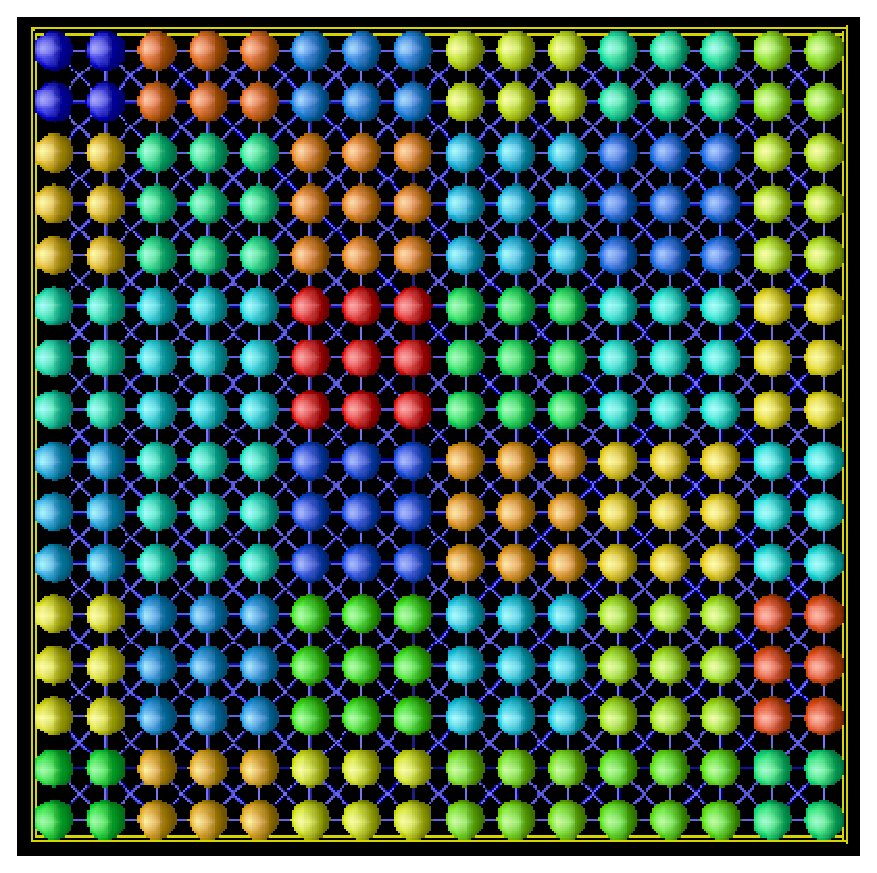
\includegraphics[height=6cm]{ml_Uncoupled-16x16.ps} \hspace{0.5cm}
  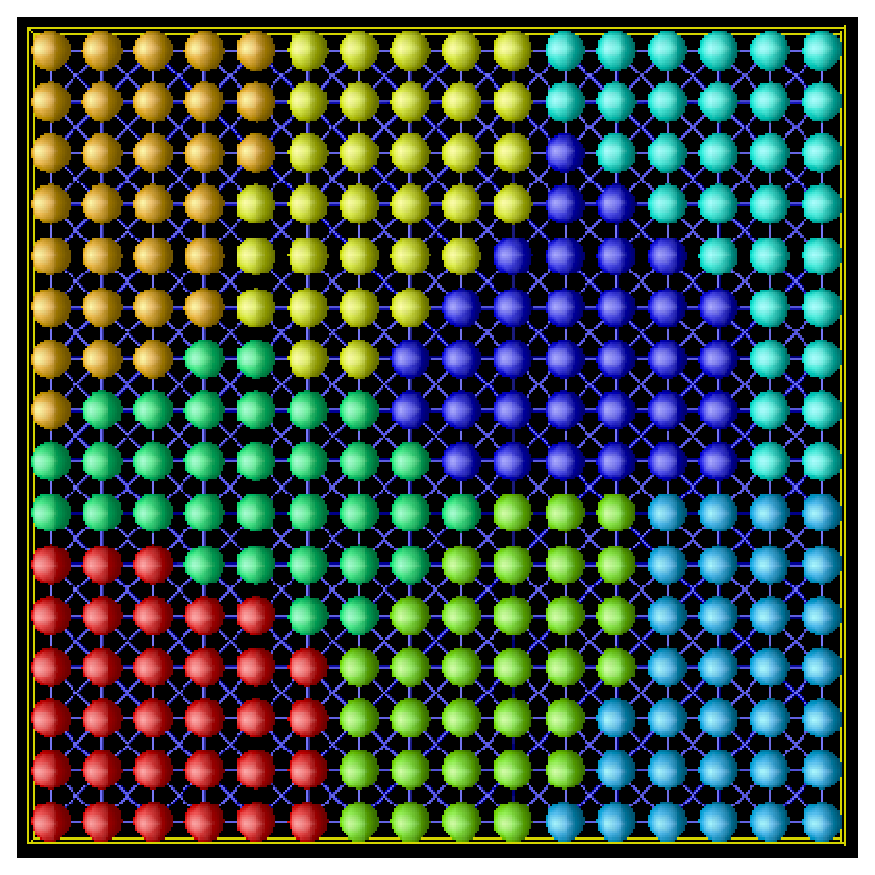
\includegraphics[height=6cm]{ml_METIS-16x16.ps}
  \caption{Aggregates for Uncoupled (left) and METIS (right) for a 16x16 Cartesian grid.}
  \label{fig:ml:comparison}
\end{figure}

\begin{table}
\begin{center}
\begin{tabular}{ | p{5cm} | p{10cm} | }
\hline
\verb!Uncoupled! & For a $1$,$2$,or $3$ dimensional structured Cartesian grid 
                   with a $3$, $9$ or $27$ point stencil respectively,
                   construct aggregates of optimal size such that
                   each aggregate resides on one processor.\\
\verb!MIS! & Maximal independent set based coarsening with aggregates
             allowed to reside on multiple processes. 
             The scheme minimizes the number of iterations,
             but the cost per iteration is high.  \\
\verb!METIS! & Use a serial graph partitioner to create
               aggregates residing on one processor. 
               The number of nodes in each aggregate
               is specified with the option {\tt aggregation: nodes per aggregate}.
               ML must be configured with {\tt --with-ml\_metis}. \\
\verb!ParMETIS! & Use a parallel graph partitioner to create aggregates that
                  may reside on multiple processors.  
                  ML must be configured with {\tt --with-ml\_parmetis3x}. 
                  The number of aggregates is
                  specified by option {\tt aggregation: global number}. \\
\hline
\end{tabular}
\caption{ML\_Epetra::MultiLevelPreconditioner Coarsening Schemes}
\label{tab:ml:aggr}
\end{center}
\end{table}

\begin{table}
\begin{center}
\begin{tabular}{ | p{5cm} | p{10cm} | }
\hline
\verb!Jacobi! & Point-Jacobi. Damping factor is specified using
{\tt smoother: damping factor}, and the number of sweeps with {\tt
  smoother: sweeps} \\ 
\verb!Gauss-Seidel! & Point Gauss-Seidel. \\
\verb!aztec! & Use AztecOO's built-in preconditioning functions as
smoothers. Or, use approximate solutions with AztecOO as smoothers. 
The AztecOO vectors \verb!options! and {\tt params} can be set using
{\tt smoother: aztec options} and {\tt smoother: aztec params}. \\
\hline
\end{tabular}
\caption{ML\_Epetra::MultiLevelPreconditioner Smoothers} 
\label{tab:ml:smoother}
\end{center}
\end{table}

\begin{table}
\begin{center}
\begin{tabular}{ | p{5cm} | p{10cm} | }
\hline
\verb!Jacobi! & Use Jacobi as a solver. \\
\verb!Gauss-Seidel! & Use Gauss-Seidel as a solver. \\
\verb!Amesos_KLU! & Use Amesos's KLU sequential solver. \\
\verb!Amesos_UMFPACK! & Use UMFPACK. \\
\verb!Amesos_Superludist! & Use SuperLU\_DIST. \\
\verb!Amesos_MUMPS! & Use MUMPS. \\
\hline
\end{tabular}
\caption{ML\_Epetra::MultiLevelPreconditioner Coarsest Grid Exact Solvers
  To use Amesos, ML must be configured with {\tt with-ml\_amesos} 
  and Amesos also be configured as needed.}
\label{tab:ml:coarse}
\end{center}
\end{table}

A very simple fragment of code using this class is reported below.
The reader may refer to file
\verb!$ML_HOME/examples/ml_example_epetra_preconditioner.cpp! for a more
complex example. To run example, first 
configure ML \verb!--with-ml_triutils!.
\begin{verbatim}
#include "ml_include.h"
#include "ml_epetra_preconditioner.h"
#include "Teuchos_ParameterList.hpp"

...

  // A is an Epetra_RowMatrix derived class object
  // solver is an AztecOO object

  Teuchos::ParameterList MList;

  // default values for smoothed aggregation
  ML_Epetra::SetDefaults("SA",MLList);
  MLList.set("max levels",6);
  MLList.set("increasing or decreasing","decreasing");
  MLList.set("aggregation: type", "MIS");
  MLList.set("coarse: type","Amesos_KLU");
  
  ML_Epetra::MultiLevelPreconditioner * MLPrec = 
    new ML_Epetra::MultiLevelPreconditioner(A, MLList, true);

  solver.SetPrecOperator(MLPrec);
  solver.SetAztecOption(AZ_solver, AZ_gmres);
  solver.Iterate(Niters, 1e-12);

  ...

  delete MLPrec;
\end{verbatim}
The general procedure is as follows. First, the user defines a Teuchos
parameters' list. Second input parameters are set via method
\verb!set(ParameterName,ParameterValue)!, where \verb!ParameterName! is
a string defining the parameter, and \verb!ParameterValue! is the
specified parameter, that can be any C++ object or pointer.  This list
is passed to the constructor, together with a pointer to the matrix, and
a boolean flag.  If this flag is set to \verb!false!, the constructor
will not compute the multilevel hierarchy until when
\verb!MLPrec->ComputePreconditioner()! is called. The hierarchy can be
destroyed using \verb!MLPrec->Destroy()!.  For instance, the user may
define a code like:
\begin{verbatim}
  // A is still not filled with numerical values
  ML_Epetra::MultiLevelPreconditioner * MLPrec = 
    new ML_Epetra::MultiLevelPreconditioner(A, MLList, false);
  
  // compute the elements of A
  ...
  // now compute the preconditioner
  MLPrec->ComputePreconditioner();

  // solve the linear system, and refill A
  ...
  MLPrec->Destroy(); // destroy previous preconditioner,
  MLPrec->ComputePreconditioner(); // and build a new one
\end{verbatim}
In this fragment of code, the user defines the ML preconditioner, but
does not create the preconditioner in the construction phase. This is of
particular interest, for example, when ML is used in conjunction with
nonlinear solvers (like NOX~\cite{NOX-home-page}).

We point out that the input parameter list is {\sl copied} in the
construction phase, hence later changes to \verb!MLList! will not affect
the preconditioner. Should one need to modify parameters in the
\verb!MLPrec!'s internally stored parameter list, proceed as
follows:
\begin{verbatim}
  ParameterList & List = MLPrec->GetList();
\end{verbatim}
and then directly modify \verb!List!.

\medskip

All ML options can have a common prefix, specified by the
user in the construction phase. For example, suppose that we require
\verb!ML: ! to be the prefix. The constructor will be
\begin{verbatim}
  MLLIst.set("ML: aggregation: type", "METIS");
  ML_Epetra::MultiLevelPreconditioner * MLPrec = 
  new ML_Epetra::MultiLevelPreconditioner(*A,  
                                          MLList, 
                                          true, 
                                          Prefix);
\end{verbatim}
where \verb!Prefix! is a char array containing \verb!ML: !.

Note that spaces are important: Do not include leading or trailing
spaces, and separate words by just one space! Misspelled parameters will
not be used, and can be detected calling method \verb!PrintUnused()!
{\sl after} the construction of the multilevel hierarchy. 

For a detailed list of all the parameters, we refer to the ML user's
guide.  Here, we report the most used parameters in
Tables~\ref{tab:ml:aggr}, \ref{tab:ml:smoother} and \ref{tab:ml:coarse}.


%%%
%%%
%%%


\subsection{Two-Level Domain Decomposition Preconditioners with ML}
\label{sec:ml_DD}

The idea of two level domain decomposition is to use a graph partitioner
to partition the graph (or mesh) into subdomains, and then treat
each subdomain as a large aggregate.
Something new happens here concerning external libraries.
Aztec00 for example contains the library Y12M, which may or may
not be compiled with Aztec00, but is available with the source code.
ML may call an external library that is not available with the source code,
and is only available as a user supplied external library.

The example contained herein 
uses the graph decomposition library METIS to create the coarse-level matrix.
If you don't have METIS, or just do not want to
re-configure ML, you may run the example 
you will be limited to use only one aggregate per process.
There are three changes to the Trilinos configuration.
One flag tells the package (ML) to look for an external library,
and the other two flag tells the compiler
where to find the include directories and external library.
Configure ML with the flags \verb!--with-ml_metis!,
and with {\tt --with-incdirs} and {\tt --with-ldflags}
set to the locations of the METIS include files and library. 
Please type {\tt configure --help} in the ML subdirectory for more information. 

Two-level domain decomposition methods are
effective for the iterative solution of many different kinds of linear
systems.  For some classes of problems, a very convenient way to define
the coarse grid operator is to use an aggregation procedure. This is very
close to what presented in Section~\ref{sec:ml_prec}. The main
difference is that only two level methods are considered, and that the
coarse grid remains of (relatively) small size. The idea is to define a
small number of aggregates on each process, using a graph decomposition
algorithm (as implemented in the library METIS, for
instance)\footnote{Aggregation schemes based on ParMETIS are also
available. Please refer to the help of the ML {\tt configure} for more
details.}. This can be done as follows.

The linear system matrix \verb!A!, here coded as an Epetra\_CrsMatrix,
corresponds to the descretization of a 2D Laplacian on a Cartesian
grid. \verb!x! and \verb!b! are the solution vector and the right-hand
side, respectively.

The AztecOO linear problem is defined as
\begin{verbatim}
  Epetra_LinearProblem problem(&A, &x, &b);
  AztecOO solver(problem);
\end{verbatim}

At this point, we can create the Teuchos parameters' list, with the
following parameters:
\begin{verbatim}
  ParameterList MLList;

  ML_Epetra::SetDefatuls(("DD",MLList);

  MLList.set("max levels",2);
  MLList.set("increasing or decreasing","increasing");

  MLList.set("aggregation: type", "METIS");
  MLList.set("aggregation: nodes per aggregate", 16);
  MLList.set("smoother: pre or post", "both");
  MLList.set("coarse: type","Amesos_KLU");
  MLList.set("smoother: type", "aztec");
\end{verbatim}
The last option tells ML to use the Aztec preconditioning function as a
smoother. Aztec requires an integer vector \verb!options! and a double
vector \verb!params!. Those can be defined as follows:
\begin{verbatim}
  int options[AZ_OPTIONS_SIZE];
  double params[AZ_PARAMS_SIZE];
  AZ_defaults(options,params);
  options[AZ_precond] = AZ_dom_decomp;
  options[AZ_subdomain_solve] = AZ_icc;
  MLList.set("smoother: aztec options", options);
  MLList.set("smoother: aztec params", params);
\end{verbatim}
Note that {\sl all} Aztec preconditioners can be used as smoothers for
ML. 
At this point we can create the ML preconditioner as
\begin{verbatim}
  ML_Epetra::MultiLevelPreconditioner * MLPrec =
    new ML_Epetra::MultiLevelPreconditioner(A, MLList, true);
\end{verbatim}
and check that no options have been misspelled, using
\begin{verbatim}
  MLPrec->PrintUnused();
\end{verbatim}
AztecOO solver is called using
\begin{verbatim}
  solver.SetPrecOperator(MLPrec);

  solver.SetAztecOption(AZ_solver, AZ_cg_condnum);

  int Niters = 500;
  solver.SetAztecOption(AZ_kspace, 160);

  solver.Iterate(Niters, 1e-12);
\end{verbatim}
Finally, some (limited) information about the preconditioning phase are
obtained using
\begin{verbatim}
  cout << MLPrec->GetOutputList();
\end{verbatim}
The entire code is reported in 
\newline
\TriExe{ml/ex2.cpp}.
\newline


\clearpage
\newpage
%@HEADER
% ************************************************************************
% 
%          Trilinos: An Object-Oriented Solver Framework
%              Copyright (2001) Sandia Corporation
% 
% Under terms of Contract DE-AC04-94AL85000, there is a non-exclusive
% license for use of this work by or on behalf of the U.S. Government.
% 
% This program is free software; you can redistribute it and/or modify
% it under the terms of the GNU General Public License as published by
% the Free Software Foundation; either version 2, or (at your option)
% any later version.
%   
% This program is distributed in the hope that it will be useful, but
% WITHOUT ANY WARRANTY; without even the implied warranty of
% MERCHANTABILITY or FITNESS FOR A PARTICULAR PURPOSE.  See the GNU
% General Public License for more details.
%   
% You should have received a copy of the GNU General Public License
% along with this program; if not, write to the Free Software
% Foundation, Inc., 675 Mass Ave, Cambridge, MA 02139, USA.
% 
% Questions? Contact Michael A. Heroux (maherou@sandia.gov)
% 
% ************************************************************************
%@HEADER

\section{Interfacing Direct Solvers with Amesos}
\label{chap:amesos}

The Amesos package provides an object-oriented interface to several
direct sparse solvers. Amesos will solve (using a direct factorization
method) the linear systems of equations
\begin{equation}
\label{eq:amesos_ls}
A X = B
\end{equation}
where $A$ is stored as an Epetra\_RowMatrix object, and $X$ and $B$ are
Epetra\_MultiVector objects.

The Amesos package has been designed to face some of the challenges of
direct solution of linear systems. In fact, many solvers have been
proposed in the last years, and often each of them requires different
input formats for the linear system matrix. Unfortunately, it is not
uncommon that the interface changes between revisions. Amesos aims to
solve those problems, furnishing a clean, consistent interface to many
direct solvers.

Using Amesos, users can interface their codes with a (large) variety of
direct linear solvers, sequential or parallel, simply by a code
instruction of type
\begin{verbatim}
AmesosProblem.Solver();
\end{verbatim}
Amesos will take care of redistributing data among the processors, if
necessary.

This Chapter starts with few notes on the installation of the third-part
packages required by Amesos. Then, the Chapter will present the use of
Amesos objects, to interface with the following packages:
\begin{itemize}
\item UMFPACK, version 4.1 (in Section~\ref{sec:umfpack});
\item SuperLUdist, version 2.0 (in Section~\ref{sec:superludist}).
\end{itemize}

%%%
%%%
%%%

\subsection{Installation of Trilinos third-part Packages}
\label{sec:3pl}

Amesos is an interface to other packages, mainly developed outside the
Trilinos framework\footnote{Currently, SuperLU is included in the
  Trilinos framework.}. In order to use those packages, the user should
check carefully copyright and licensing of those third party codes.
Please refer to the web page for the package that you are interested in
for details. Amesos supports a variety of direct solvers for linear
systems of equations, and you are likely to use Amesos with only few of
them. We suggest to define the shell variable \verb!TRILINOS_3PL!  to
define the directory used to stored third-part packages. For instance,
under BASH you may have a line of type
\begin{verbatim}
export TRILINOS_3PL=/home/msala/Trilinos3PL
\end{verbatim}
in your \verb!.bashrc! file. Then, you may decide to create a directory
to hold include files and libraries. For instance, to run LINUX with
MPI:
\begin{verbatim}
$ mkdir ${TRILINOS_3PL}/LINUX_MPI
$ mkdir ${TRILINOS_3PL}/LINUX_MPI/include
$ mkdir ${TRILINOS_3PL}/LINUX_MPI/lib
\end{verbatim}
(Note that this will reflect the directory structure used by Trilinos,
see Section~\ref{sec:installing}). While installing a package, you can
now copy all include files and libraries in these directories.

Using this setting, you can configure Amesos with a command of type
\begin{verbatim}
$ cd ${TRILINOS_HOME}/packages/amesos
$ ./configure --prefix=${TRILINOS_HOME}/LINUX_MPI \
  --enable-mpi --with-mpi-compilers \
  --enable-amesos-umfpack \
  --enable-amesos-superludist \
  --with-amesos-superludistlib=\
  "${TRILINOS_3PL}/SuperLU_DIST_2.0/libsuperlu_LINUX.a"
\end{verbatim}
(This command is followed by \verb!make! and \verb!make install!, as
usual.)  This will enable UMFPACK and SuperLUdist, which are the two
packages covered in this Chapter.

For more details about the configuration options of Amesos, please refer
to Amesos documentation.

\begin{remark}
  Amesos can handle multiple right-hand side using Epetra\_MultiVectors.
\end{remark}

%%%
%%%
%%%

\subsection{UMFPACK}
\label{sec:umfpack}

File \TriExe{amesos/ex1.cpp} shows how to use Amesos to solve a linear
system with UMFPACK\footnote{UMFPACK is a set of routines solving sparse
  linear systems via LU factorization. It is copyrighted by Timothy
  A.~Davis. More information can be obtained at the web page 
  {\tt http://www.cise.ufl.edu/research/sparse/umfpack}. }.

Suppose that \verb!A!, \verb!x! and \verb!b! are an Epetra\_RowMatrix
and two Epetra\_MultiVector, respectively, or compatible dimensions.
Amesos objects for the solution of linear systems requires an
Epetra\_LinearProblem object, plus another object,
\verb!AMESOS::Parameter::List!, used to specify the parameters.
\begin{verbatim}
Epetra_LinearProblem Problem(&A,&x,&b);
AMESOS::Parameter::List params;
\end{verbatim}
Then, only few lines are required: We can define an Amesos object and
solve the problem,
\begin{verbatim}
Amesos_Umfpack UmfpackProblem(Problem,params);
UmfpackProblem.Solve();
\end{verbatim}
or, alternatively, it is possible to specify when symbolical
factorization, numerical factorization and solution occur,
\begin{verbatim}
Amesos_Umfpack UmfpackProblem(Problem,params); 
UmfpackProblem.SymbolicFactorization();
UmfpackProblem.NumericFactorization();
UmfpackProblem.Solve();
\end{verbatim}
Note that {\sl exactly} the same code can be run with more than one
processor. In this case, being UMFPACK a serial solver, Amesos will take
care to gather all required data on a processor, solve sequentially
the linear system, and then broadcast the solution.

%%%
%%%
%%%

\subsection{SuperLUdist}
\label{sec:superludist}

Solving using SuperLUdist\footnote{SuperLU\_DIST is a parallel extension
  to the  serial SuperLU library.   It  is targeted for the  distributed
  memory parallel  machines. 
Copyright (c) 2003, The Regents of the University of California, through
Lawrence Berkeley National Laboratory.
Please refer
  to  the  web site {\tt  http://www.nersc.gov/~xiaoye/SuperLU} for more
  information.}  is not   much  different    from  what presented     in
Section~\ref{sec:umfpack}.    Instead of   declaring  an Amesos\_Umfpack
object, one can proceed as follows:
\begin{verbatim}
Amesos_Superludist * SuperludistProblem = 
 new Amesos_Superludist(Problem,params);
\end{verbatim}
followed by a call to Solve(), possibly preceded by
SymbolicFactorization() and NumericFactorization().

\begin{remark}
  We have declared a pointer to and Amesos\_Superludist object because
  the destructor of this object contains some MPI
  calls. As in example \newline \TriExe{amesos/ex2.cpp} the destructor is called
  at the end of the main function (after a call to
  \verb!MPI_Finalize()!, we have to delete this object using the C++
  statement
\begin{verbatim}
delete SuperludisProblem;
\end{verbatim}
  before the call to \verb!MPI_Finalize()!.
\end{remark}

%%%
%%%
%%%

\subsection{A Generic Interface to Various Direct Solvers}
\label{sec:amesos_generic}

All Amesos objects are derived from the Amesos\_BaseClass object. Using
the capabilities of C++, one may decide to code a generic interface to a
direct solver as follows:
\begin{verbatim}
// parameter vector for Amesos
AMESOS::Parameter::List ParamList;

// prepare the linear solver
Amesos_BaseSolver * AmesosProblem;

switch( choice ) {
case ML_SOLVE_WITH_AMESOS_UMFPACK:
    AmesosProblem = new Amesos_Umfpack( *LinearProblem, ParamList );
    break;
  case ML_SOLVE_WITH_AMESOS_SUPERLUDIST:
    AmesosProblem = new Amesos_Superludist( *LinearProblem, ParamList );
    break;
  default:
    cerr << ``Error'' << endl;
}
\end{verbatim}

Now, factorization and solution are the same for all the packages:
\begin{verbatim}  
AmesosProblem->SymbolicFactorization();
AmesosProblem->NumericFactorization();
AmesosProblem = (void *) AmesosProblem ;
\end{verbatim}




\clearpage
\newpage
%@HEADER
% ************************************************************************
% 
%          Trilinos: An Object-Oriented Solver Framework
%              Copyright (2001) Sandia Corporation
% 
% Under terms of Contract DE-AC04-94AL85000, there is a non-exclusive
% license for use of this work by or on behalf of the U.S. Government.
% 
% This program is free software; you can redistribute it and/or modify
% it under the terms of the GNU General Public License as published by
% the Free Software Foundation; either version 2, or (at your option)
% any later version.
%   
% This program is distributed in the hope that it will be useful, but
% WITHOUT ANY WARRANTY; without even the implied warranty of
% MERCHANTABILITY or FITNESS FOR A PARTICULAR PURPOSE.  See the GNU
% General Public License for more details.
%   
% You should have received a copy of the GNU General Public License
% along with this program; if not, write to the Free Software
% Foundation, Inc., 675 Mass Ave, Cambridge, MA 02139, USA.
% 
% Questions? Contact Michael A. Heroux (maherou@sandia.gov)
% 
% ************************************************************************
%@HEADER

\section{Eigenvalue and Eigenvector Computations with Anasazi}
\label{chap:anasazi}

The Anasazi package has been designed as an extensible and
interoperable framework for large-scale eigenvalue algorithms. Anasazi
provides a generic interface to a collection of algorithms for solving
large-scale eigenvalue problems. Anasazi requires matrices and vectors
to be derived from abstract classes, and therefore it can be used with
any matrix and vector classes that implement these interfaces. The
algorithms currently available through Anasazi are a block Krylov
Schur method and a block Davidson method.

In this Chapter we present:
\begin{itemize}
\item a description of the Anasazi framework (Section~\ref{sec:anasazi:framework}),
\item the interface to the Epetra linear algebra package (Section~\ref{sec:anasazi:interface}), and
\item an example using Anasazi for the solution of an eigenvalue problem 
(Section~\ref{sec:anasazi:example}).
\end{itemize}

%%%
%%%
%%%
\subsection{Anasazi Framework}
\label{sec:anasazi:framework}


The two most important classes in Anasazi are \verb!Eigenproblem! and
\verb!Eigensolver!. The \verb!Anasazi::Eigenproblem! class defines an interface
to provide all of the information necessary to compute the solution to an
eigenproblem. The \verb!Anasazi::Eigensolver! class defines the minimum
interface required of eigensolvers in Anasazi. Eigensolvers are implemented by
subclassing the \verb!Anasazi::Eigensolver! abstract class. The solvers
available in the current version of Anasazi are listed in
Table~\ref{tab:anasazi:solvers}.


\begin{table}[htp]
\begin{center}
\begin{tabular}{| p{4cm} p{8cm} |}
\hline
Solver & Description \\
\hline
{\tt BlockDavidson}    & A block Davidson solver for symmetric
                         eigenvalue problems.\\
{\tt BlockKrylovSchur} & A block Krylov Schur solver for symmetric or
                         nonsymmetric problems.\\
\hline
\end{tabular}
\caption{Current eigensolvers implemented in Anasazi.}
\label{tab:anasazi:solvers}
\end{center}
\end{table}


Both the eigenproblem and the eigensolver in Anasazi are templated according to
the scalar type, the multivector type, and the operator type. The scalar type
must satisfy the interface defined by \verb!Teuchos::ScalarTraits! (see
Section~\ref{sec:teuchos:ScalarTraits}). Both the operators and the
multivectors are considered to be opaque objects. That is, only knowledge of
the matrix and vectors via elementary operations is necessary. The required
operations are specified by the interfaces \verb!MultiVecTraits! and
\verb!OperatorTraits!. An implementation of Anasazi is accomplished via use of
these interfaces. 

This flexibility allows Anasazi to utilize existing linear algebra
codes. For example, with regard to a multivector class, there are
three choices for implementing Anasazi:
\begin{itemize}
\item define a specialization of an existing class which satisfies the
\verb!MultiVecTraits! class,
\item create a subclass of \verb!Anasazi::MultiVec!, for which a
\verb!MultiVecTraits! specialization is already defined by Anasazi, or
\item use the Epetra class \verb!Epetra_MultiVector!, for which a
\verb!MultiVecTraits! specialization is already defined.
\end{itemize}

Similar to the multivector class, there are three approaches for
implementing Anasazi with regard to the linear operators:
\begin{itemize}
\item define a specialization satisfying \verb!OperatorTraits!,
\item subclass the \verb!Anasazi::Operator! abstract class, for which a
\verb!OperatorTraits! specialization already exists, or
\item use a subclass of \verb!Epetra_Operator!, 
for which a \verb!OperatorTraits! specialization is already defined.
\end{itemize}

The first and second approaches are outside the scope of this
tutorial. The third of these is the simplest and allows the usage of
any other Trilinos packages which recognize the Epetra multivector
class. The usage of the Epetra interfaces is discussed in the next
section.

Having chosen classes for the multivector and the operator, it remains
to specify the operators and initial vectors to define the eigenvalue
problem, to specify the options for the eigensolver, and to solve the
problem. Specifying the eigenvalue problem consists mainly of setting
the operators associated with the specific problem and specifying the
symmetry of the problem. 

For the eigensolver, we must first choose which eigensolver to use.  Then any
options for the eigensolver must be put into a \verb!Teuchos::ParameterList!
class (see Section~\ref{sec:teuchos:ParameterList}) and passed to the
eigensolver, along with the eigenproblem. Anasazi also makes use of the
\verb!Teuchos::RefCountPtr! smart-pointers
(Section~\ref{sec:teuchos:RefCountPtr}). Familiarity with these utility classes
will be helpful when using Anasazi. Finally, the eigensolver may also take as
an argument an instance of \verb!Anasazi::SortManager!, to determine which
eigenvalues are targeted by the solver. Usage of these classes are illustrated
in Section~\ref{sec:anasazi:example}.


%%%
%%%
%%%
\subsection{Using the Epetra interface to Anasazi}
\label{sec:anasazi:interface}

In order to use the Epetra interface to Anasazi, the user must include
the following files:
\begin{verbatim}
#include "AnasaziEpetraAdapter.hpp"
#include "AnasaziBasicEigenproblem.hpp"
\end{verbatim}
In addition, the user will need one of the following, depending on
whether MPI is used or not:
\begin{verbatim}
#include "Epetra_MpiComm.h"
#include "Epetra_SerialComm.h"
\end{verbatim}
For more information about the \verb!Epetra_Map! and \verb!Epetra_Comm!
classes, see the tutorial section covering Epetra (Sections~\ref{sec:comm} and
\ref{sec:map}).

Because Epetra makes exclusive use of double precision arithmetic,
choosing \verb!Epetra_Operator!  and \verb!Epetra_MultiVector!  makes
sense when the scalar type for the eigenproblem/solver is
\verb!double!. For brevity, we will declare type definitions for the
multivector type and operator type:
\begin{verbatim}
typedef Epetra_MultiVector MV;
typedef Epetra_Operator OP;
\end{verbatim}

We can now declare an eigenvalue problem and a solver, subclasses of
the following abstract classes:
\begin{verbatim}
Anasazi::Eigenproblem<double,MV,OP>
Anasazi::Eigensolver<double,MV,OP>
\end{verbatim}

An example defining an eigenvalue problem and solving the problem
using an Anasazi eigensolver is given in the next section.

%%%
%%%
%%%
\subsection{Defining and Solving an Eigenvalue Problem}
\label{sec:anasazi:example}

The first step in solving an eigenvalue problem is to define the eigenvalue
problem. Assume we have chosen classes to represent our scalars, multivectors
and operators, as \verb!ST!, \verb!MV! and \verb!OP!, respectively. Given an
operator \verb!A! and a multivector \verb!X! to initialize the problem, both
wrapped in \verb!Teuchos::RefCountPtr!s, we might define the eigenproblem as
follows:
\begin{verbatim}
Teuchos::RefCountPtr< BasicEigenproblem<ST,MV,OP> > MyProblem 
  = Teuchos::rcp( new BasicEigenproblem<ST,MV,OP>(A,X) );
MyProblem->SetSymmetric( true );
MyProblem->SetNEV( 5 );
MyProblem->SetProblem();
\end{verbatim}

The first line creates a \verb!BasicEigenproblem! object and wraps it
in a Teuchos smart-pointer. The second line specifies the symmetry of
the eigenproblem, information which may be utilized by the eigensolver
for extra efficiency. The third line specifies the desired number of
eigenvalues and eigenvectors. Lastly, the fourth signals that we have
finished setting up the eigenproblem. This step must be completed
before attempting to solve the problem.

Let us, for example, attempt to solve this eigenvalue problem with a
block Krylov Schur solver. First, we declare a sort manager to specify the
targeted eigenvalues:
\begin{verbatim}
std::string which("SM");
Teuchos::RefCountPtr<Anasazi::BasicSort<ST,MV,OP> > MySM =
  Teuchos::rcp( new Anasazi::BasicSort<ST,MV,OP>(which) );
\end{verbatim}
The option chosen was \verb!"SM"!, signaling that we want to compute
the eigenvalues with the smallest magnitude. Other options for the
\verb!Anasazi::BasicSort! sort manager are listed in
Table~\ref{tab:anasazi:sm}.

\begin{table}
\begin{center}
\begin{tabular}{| p{2cm} l |}
\hline
Option & Action \\
\hline
{\tt SM} & Sort eigenvalues in increasing order of magnitude \\
{\tt SR} & Sort eigenvalues in increasing order of real part \\
{\tt SI} & Sort eigenvalues in increasing order of imaginary part \\
{\tt LM} & Sort eigenvalues in decreasing order of magnitude \\
{\tt LR} & Sort eigenvalues in decreasing order of real part \\
{\tt LI} & Sort eigenvalues in decreasing order of imaginary part \\
\hline
\end{tabular}
\caption{Options for Anasazi::BasicSort.}
\label{tab:anasazi:sm}
\end{center}
\end{table}

Next we create an output manager, specifying the verbosity of the
solver:
\begin{verbatim}
Teuchos::RefCountPtr<Anasazi::OutputManager<ST> > MyOM = 
  Teuchos::rcp(  new Anasazi::OutputManager<ST>( MyPID ) );
MyOM->SetVerbosity( Anasazi::Error+Anasazi::Warning );
\end{verbatim}
Here, we have asked for information regarding errors and warnings from
the eigensolver. Other available information is listed in
Table~\ref{tab:anasazi:om}.

\begin{table}
\begin{center}
\begin{tabular}{| p{7cm} l |}
\hline
Option & Action \\
\hline
{\tt Anasazi::Error} & 
  This option is always set \\
{\tt Anasazi::Warning} & 
  Warnings \\
{\tt Anasazi::IterationDetails} & 
  Details at each iteration \\
{\tt Anasazi::OrthoDetails} & 
  Details about orthogonality \\
{\tt Anasazi::FinalSummary} & 
  A final summary \\
{\tt Anasazi::Debug} & 
  Debugging information \\
\hline
\end{tabular}
\caption{Options for Anasazi::OutputManager.}
\label{tab:anasazi:om}
\end{center}
\end{table}

We also will specify the parameters for the eigensolver:
\begin{verbatim}
Teuchos::ParameterList MyPL;
MyPL.set( "Block Size", 5 );
MyPL.set( "Max Blocks", 5 );
MyPL.set( "Max Restarts", 100 );
MyPL.set( "Tol", 1.0e-8 );
\end{verbatim}
Different eigensolvers allow different parameters.
Tables~\ref{tab:anasazi:bksparams} and \ref{tab:anasazi:bdparams} list
the settings for the block Krylov Schur and block Davidson solvers.


\begin{table}
\begin{center}
\begin{tabular}{| p{4cm} l |}
\hline
Parameter & Default \\
\hline
{\tt Block Size}   & 1      \\
{\tt Max Blocks}   & 25     \\
{\tt Max Restarts} & 0      \\
{\tt Step Size}    & Block\_Size*Max\_Blocks*(Max\_Restarts+1) \\
{\tt Tol}          & 1.0e-6 \\
\hline
\end{tabular}
\caption{Options for Anasazi::BlockKrylovSchur}
\label{tab:anasazi:bksparams}
\end{center}
\end{table}


\begin{table}
\begin{center}
\begin{tabular}{| p{4cm} l |}
\hline
Parameter & Default \\
\hline
{\tt Block Size} & 1      \\
{\tt Max Blocks} & 25     \\
{\tt Max Iters}  & 300    \\
{\tt Tol}        & 1.0e-6 \\
\hline
\end{tabular}
\caption{Options for Anasazi::BlockDavidson}
\label{tab:anasazi:bdparams}
\end{center}
\end{table}

We now have all of the information needed to declare the eigensolver
and solve the problem.
\begin{verbatim}
Anasazi::BlockKrylovSchur<ST,MV,OP> 
  MySolver( MyProblem, MySM, MyOM, MyPL );
\end{verbatim}
The eigenproblem is solved with the instruction
\begin{verbatim}
Anasazi::ReturnType sret = MySolver.solve();
\end{verbatim}
The return value of the solver indicates whether the algorithm
succeeded or not. Potential values are listed in
Table~\ref{tab:anasazi:rt}.

\begin{table}
\begin{center}
\begin{tabular}{| p{4cm} l |}
\hline
Parameter & Default \\
\hline
Anasazi::Ok          & Success. \\
Anasazi::Unconverged & Solver did not converge to specified accuracy. \\
Anasazi::Failed      & An error with the input or in the solver. \\
\hline
\end{tabular}
\caption{Anasazi::ReturnType values.}
\label{tab:anasazi:rt}
\end{center}
\end{table}

A summary of results can be printed on the screen:
\begin{verbatim}
MySolver.currentStatus();
\end{verbatim}
Eigenvectors and eigenvalues can be retrieved using
\begin{verbatim}
Teuchos::RefCountPtr<Epetra_MultiVector >  evecs 
   = MyProblem->GetEvecs();
Teuchos::RefCountPtr<std::vector<double> > evals 
   = MyProblem->GetEvals();
\end{verbatim}
For a nonsymmetric problem with potentially complex eigenvalues and
eigenvectors, \verb!evecs! and \verb!evals! contain both the real and
complex parts of these, as described in the comments of
\TriExe{anasazi/ex1.cpp}.

Example \TriExe{anasazi/ex1.cpp} shows how to compute the eigenvectors
corresponding to the lowest eigenvalues for a 2D Laplace problem using
the block Krylov Schur solver.  Example \TriExe{anasazi/ex2.cpp}
solves this example, using instead the block Davidson eigensolver.
Finally, the block Krylov Schur solver is used to solve a nonsymmetric
convection-diffusion problem in Example \TriExe{anasazi/ex3.cpp}.

%Table~\ref{tab:anasazi:exLapl} reports the lower
%eigenvalues. 

%\begin{figure}[htbp]
%  \centering
%  \includegraphics[height=6cm]{anasazi_Laplace_1D.ps}
%  \caption{Lowest eigenvalues of a 1D Laplace problem, with $h=1/33$.}
%  \label{fig:anasazi:1D}
%\end{figure}

%\begin{table}[htbp]
%  \centering
%  \begin{tabular}{| l | c |}    
%    \hline
%& {\tt laplace\_2d} \\
%     \hline
%     $h = 1/33$  & 0.00905   & 0.0181    & 0.02716  \\
%     $h = 1/65$  & 0.00235   & 0.00467   & 0.007006 \\
%     $h = 1/129$ & 0.0005936 & 0.0011861 & -        \\
%     $h = 1/257$ & 0.000149  & 0.0002983 & -        \\
%     $h = 1/513$ & 3.75e-5   & -         & -        \\
%     \hline
%  \end{tabular}
%  \caption{$\lambda_{min}$ for 1D, 2D and 3D Laplace problem on a Cartesian mesh.}
%  \label{tab:anasazi:exLapl}
%\end{table}
%%%
%%%
%%%



% FIXME
%\subsection{Concluding Remarks on Anasazi}
%\label{sec:anasazi_concluding}

%More documentation on the Anasazi package can be found in
%\cite{Anasazi-Ref-Guide,Anasazi-User-Guide}.



\clearpage
\newpage
%@HEADER
% ************************************************************************
% 
%          Trilinos: An Object-Oriented Solver Framework
%              Copyright (2001) Sandia Corporation
% 
% Under terms of Contract DE-AC04-94AL85000, there is a non-exclusive
% license for use of this work by or on behalf of the U.S. Government.
% 
% This program is free software; you can redistribute it and/or modify
% it under the terms of the GNU General Public License as published by
% the Free Software Foundation; either version 2, or (at your option)
% any later version.
%   
% This program is distributed in the hope that it will be useful, but
% WITHOUT ANY WARRANTY; without even the implied warranty of
% MERCHANTABILITY or FITNESS FOR A PARTICULAR PURPOSE.  See the GNU
% General Public License for more details.
%   
% You should have received a copy of the GNU General Public License
% along with this program; if not, write to the Free Software
% Foundation, Inc., 675 Mass Ave, Cambridge, MA 02139, USA.
% 
% Questions? Contact Michael A. Heroux (maherou@sandia.gov)
% 
% ************************************************************************
%@HEADER

\section{Solving Nonlinear Systems with NOX}
\label{chap:nox}

NOX is a suite of solution methods for the solution of nonlinear
systems of type
\begin{equation}
\label{eq:nonlinear}
F(x) = 0,
\end{equation}
with
\[
F(x) = 
\begin{pmatrix}
  f_1(x_1, \ldots, x_n) \\
  \vdots \\
  f_n(x_1, \ldots, x_n) \\
\end{pmatrix}
\]
is a nonlinear vector function. The Jacobian matrix of $F$, $J$, is
defined by
\[
J_{i,j} = \frac{ \partial F_i}{\partial x_j} (x).
\]

NOX aims to solver (\ref{eq:nonlinear}) using Newton-type methods. NOX
uses an abstract vector and ``group'' interface. Current implementation
are provided for Epetra/AztecOO objects, but also for LAPACK and PETSc.
It provides various strategies for the solution of nonlinear systems,
and it has been designed to be easily integrated into existing
applications.

In this Chapter, we will
\begin{itemize}
\item Outline the basic issued of the  solution of nonlinear
  systems (in Section~\ref{sec:nox_theoretical});
\item Introduce the NOX package (in Section \ref{sec:nox_intro});
\item Describe how to introduce a NOX solver in an existing code (in
  Section \ref{sec:nox_introduce});
\item Present Jacobian-free methods (in
  Section~\ref{sec:nox_jacobian_free}).
\end{itemize}

%%%
%%%
%%%

\subsection{Theoretical Background}
\label{sec:nox_theoretical}

Aim of this Section is to briefly present some aspects of the solution
of nonlinear systems, to establish a notation. The Section is not
supposed to be exhaustive, nor complete on this subject. The reader is
referred to the existing literature for a rigorous presentation.

\medskip

To solve system of nonlinear equations, NOX makes use of Newton-like methods.
The Newton method defines a suite $\{ x_k\}$ that, under some
conditions, converges to $x$, solution of~(\ref{eq:nonlinear}).
The algorithm is as follows: given $x_0$, for $k=1,\ldots$ until
convergence, solve
\begin{equation}
J_k  (x_{k-1})\left ( x_{k} - x_{k-1} \right) = 
- F(x_{k-1}),\quad
J_k  (x_{k-1}) =  \left[ \frac{ \partial F}{
        \partial x}( x_{k-1}) \right] .
\label{eq:newton_step}
\end{equation}
Newton method introduces a local full linearizion of the
equation. Solving a system of linear equations at each Newton step can
be very expensive if the number of unknowns is large, and may not be
justified if the current iterate is far from the solution. Therefore,
a departure from the Newton framework consists of considering {\em
inexact} Newton methods, which solve system~(\ref{eq:newton_step})
only approximatively.

In fact, in practical implementation of the Newton method, one or more
of the following approximations are used:
\begin{enumerate}
\item The Fr\'echet derivative $J_k$ for the Newton step is not
  recomputed at every Newton step;
\item The equation for the Newton step~(\ref{eq:newton_step}) is solved
  only inexactly;
\item Defect-correction methods are employed, that is, $J_k$ is
  numerically computed using low-order (in space) schemes, while the
  right-hand side is built up using high-order methods.
\end{enumerate}

For a given initial guess, ``close enough'' to the solution of
(\ref{eq:nonlinear}), the Newton method with exact linear solves
converges quadratically. In practice, the radius of convergence is often
extended via various methods. NOX provides, among others, line search
techniques and trust region strategies.

%%%
%%%
%%%

\subsection{Creating NOX Vectors and Group}
\label{sec:nox_intro}

NOX is not based on any particular linear algebra package. Users are
required to supply methods that derive from the abstract classes
\verb!NOX::Abstract::Vector! (which provides support for basic vector
operations as dot products), and \verb!NOX::Abstract::Group!  (which
supports the linear algebra functionalities, evaluation of the function
$G$ and, optionally, of the Jacobian $J$).

In order to link their code with NOX, users have to write their own
instantiation of those two abstract classes. In this tutorial, we will
consider the concrete implementations provided for Epetra matrices and
vectors. As this implementation is separate from the NOX algorithms, the
configure option \verb!--enable-nox-epetra! has to be specified (see
Section~\ref{sec:installing})\footnote{Other two concrete implementation
  are provided, for LAPACK and PETSc. The user may wish to configure NOX
  with {\tt --enable-nox-lapack} or {\tt --enable-nox-petsc}. Examples
  can be compiled with the options {\tt --enable-nox-lapack-examples},
  {\tt --enable-nox-petsc-examples}, and {\tt
    -enable-nox-epetra-exemples}.}.

%%%
%%%
%%%

\subsection{Introducing NOX in an Existing Code}
\label{sec:nox_introduce}

Two basic steps are required to implement a \verb!NOX::Epetra!
interface. First, a concrete class derived from
\verb!NOX::Epetra::Interface! has to be written. This class must define
the following methods:
\begin{enumerate}
\item A method to compute $y = F(X)$ for a given $x$. The syntax is
\begin{verbatim}
computeF(const Epetra_Vector & x, Epetra_Vector & y, 
         FillType flag)
\end{verbatim}
with \verb!x! and \verb!y! two Epetra\_Vectors, and \verb!flag! an
enumerated type that tells why this method was called. In fact, NOX has
the ability to generate Jacobians based on numerical differencing. In
this case, users may want to compute an inexact (and hopefully cheaper)
$F$, since it is only used in the Jacobian (or preconditioner).
\item A function to compute the Jacobian, whose syntax is
\begin{verbatim}
computeJacobian(const Epetra_Vector & x, 
                Epetra_Operator * Jac)
\end{verbatim}
  This method is optional optional method. It should be implemented when
  users wish to supply their own evaluation of the Jacobian. If the user
  does not wish to supply their own Jacobian, they should implement this
  method so that it throws an error if it is called. This method should
  update the Jac operator so that subsequent Epetra\_Operator::Apply()
  calls on that operator correspond to the Jacobian at the current
  solution vector x.
\item A method which fills a preconditioner matrix, whose syntax is
\begin{verbatim}
computePrecMatrix(const Epetra_Vector & x, 
                  Epetra_RowMatrix & M)
\end{verbatim}
  It should only contain an estimate of the Jacobian. If users do not
  wish to supply their own Preconditioning matrix, they should implement
  this method such that if called, it will throw an error.
\item A method to apply the user's defined preconditioner. The syntax is
\begin{verbatim}
computePreconditioner(const Epetra_Vector & x, Epetra_Operator & M)
\end{verbatim}
  The method should compute a preconditioner based upon the solution
  vector x and store it in the Epetra\_Operator M. Subsequent calls to
  the Epetra\_Operator::Apply method will apply this user supplied
  preconditioner to epetra vectors.
\end{enumerate}

Then, the user can construct a \verb!NOX::Epetra::Group!, which contains
information about the solution technique. All constructors require:
\begin{itemize}
\item A parameter list for printing output and for input options,
  defined as \verb!NOX::Parameter::List!. 
\item An initial guess for the solution (stored in an Epetra\_Vector
  object);
\item an operator for the Jacobian and (optionally) and operator for the
  preconditioning phase. Users can write their own operators. In
  particular, the Jacobian can be defined by the user as an
  Epetra\_Operator,
\begin{verbatim}
Epetra_Operator & J = UserProblem.getJacobian(),
\end{verbatim}
created as a NOX matrix-free operator,
\begin{verbatim}
NOX::Epetra::MatrixFree & J = MatrixFree(userDefinedInterface, 
                                         solutionVec),
\end{verbatim}
or created by NOX using a finite differencing,
\begin{verbatim}
NOX::Epetra::FiniteDifference & J = FIXME...
\end{verbatim}
\end{itemize}

At this point, users have to create an instantiation of the
\verb!NOX::Epetra::Interface! derived object,
\begin{verbatim}
UserInterface interface(...),
\end{verbatim}
and finally construct the group,
\begin{verbatim}
NOX::Epetra::Group gourp(printParams, lsParams, interface, FIXME).
\end{verbatim}

%%%
%%%
%%%

%\subsection{Stopping Criteria}
%\label{sec:nox_stopping}

%NOX can check the convergence of the nonlinear solver in a variety of
%ways.
%FIXME...

%%%
%%%
%%%

\subsection{A Simple Nonlinear Problem}
\label{sec:nox_simple}

As an example. define $F : \mathbb{R}^2 \rightarrow \mathbb{R}^2$ by
\[
F(x) = 
\begin{pmatrix}
x_1^2 + x_2^2 -1 \\
x_2 - x_1^2
\end{pmatrix}.
\]
With this choice of $F$, the exact solutions of (\ref{eq:nonlinear}) are
the intersections of the unity circle and the parabola $x_2 -
x_1^2$. Simple algebra shows that one solution lies in the first
quadrant, and has coordinates
\[
\alpha = \left( \sqrt{\frac{\sqrt{5}-1}{2}}, \frac{\sqrt{5}-1}{2} \right),
\]
the other being the reflection of $\alpha$ among the $x_2$ axis.

Code \TriExe{nox/ex1.cpp} applies the Newton method to this problem,
with $x_0 = (0.5, 0.5)$ as a starting solution. The output is
approximatively as follows:
\begin{verbatim}
[msala:nox]> mpirun -np 1 ./ex1.exe
*****************************************************
-- Nonlinear Solver Step 0 --
f = 5.590e-01  step = 0.000e+00  dx = 0.000e+00
*****************************************************

*****************************************************
-- Nonlinear Solver Step 1 --
f = 2.102e-01  step = 1.000e+00  dx = 3.953e-01
*****************************************************

*****************************************************
-- Nonlinear Solver Step 2 --
f = 1.009e-02  step = 1.000e+00  dx = 8.461e-02
*****************************************************

*****************************************************
-- Nonlinear Solver Step 3 --
f = 2.877e-05  step = 1.000e+00  dx = 4.510e-03 (Converged!)
*****************************************************

*****************************************************
-- Final Status Test Results --
Converged....OR Combination ->
  Converged....F-Norm = 2.034e-05 < 2.530e-04
               (Length-Scaled Two-Norm, Relative Tolerance)
  ??...........Number of Iterations = -1 < 20
*****************************************************

-- Parameter List From Solver --
Direction ->
  Method = "Newton"   [default]
  Newton ->
    Linear Solver ->
      Max Iterations = 400   [default]
      Output ->
        Achieved Tolerance = 8.6e-17   [unused]
        Number of Linear Iterations = 2   [unused]
        Total Number of Linear Iterations = 6   [unused]
      Tolerance = 1e-10   [default]
    Rescue Bad Newton Solve = true   [default]
Line Search ->
  Method = "More'-Thuente"
  More'-Thuente ->
    Curvature Condition = 1   [default]
    Default Step = 1   [default]
    Interval Width = 1e-15   [default]
    Max Iters = 20   [default]
    Maximum Step = 1e+06   [default]
    Minimum Step = 1e-12   [default]
    Optimize Slope Calculation = false   [default]
    Recovery Step = 1   [default]
    Recovery Step Type = "Constant"   [default]
    Sufficient Decrease = 0.0001   [default]
    Sufficient Decrease Condition = "Armijo-Goldstein"   [default]
  Output ->
    Total Number of Failed Line Searches = 0   [unused]
    Total Number of Line Search Calls = 3   [unused]
    Total Number of Line Search Inner Iterations = 0   [unused]
    Total Number of Non-trivial Line Searches = 0   [unused]
Nonlinear Solver = "Line Search Based"
Output ->
  2-Norm of Residual = 2.88e-05   [unused]
  Nonlinear Iterations = 3   [unused]
Printing ->
  MyPID = 0   [default]
  Output Information = 2
  Output Precision = 3   [default]
  Output Processor = 0   [default]
Computed solution :
Epetra::Vector
     MyPID           GID               Value
         0             0                   0.786
         0             1                   0.618
Exact solution :
Epetra::Vector
     MyPID           GID               Value
         0             0                   0.786
         0             1                   0.618
\end{verbatim}

%%%
%%%
%%%

\subsection{A 2D Nonlinear PDE Problem}
\label{sec:nox_2d}

In this Section, we consider the solution of the following nonlinear PDE
problem:
\begin{equation}
  \label{eq:nox_nonlinear_2d}
  \left\{
    \begin{array}{r c l l }
      - \Delta u + \lambda e^u & = & 0 & \mbox{ in } \Omega = (0,1)
      \times (0,1) \\
      u & = & 0 & \mbox{ on } \partial \Omega .
    \end{array}
  \right.   
\end{equation}
For the sake of simplicity, we use a finite difference scheme ona
Cartesian gri, with constant mesh sizes $h_x$ and $h_y$. Using standard
procedures, the discrete equation at node $(i,j)$ reads
\[
\frac{ - u_{i-1,j} + 2 u_{i,j} - u_{i+1,j} }{ h_x^2} +
\frac{ - u_{i,j-1} + 2 u_{i,j} - u_{i,j+1} }{ h_y^2}  -
\lambda e^{u{_i,j}} = 0 .
\]

In example \TriExe{nox/ex2.cpp}, we build the Jacobian matrix as an
Epetra\_CrsMatrix, and we use NOX to solve problem
(\ref{eq:nox_nonlinear_2d}) for a given value of $\lambda$.  The example
shows how to use NOX for more complex cases. The code defines a class,
here called PDEProblem, which contains two main methods: One to compute
$F(x)$ for a given $x$, and the other to update the entries of the
Jacobian matrix. The class contains all the problem definitions (here,
the number of nodes along the x-axis and the y-axis and the value of
$\lambda$). In more complex cases, a similar class may have enough
information to compute, for instance, the entries of $J$ using a
finite-element approximation of the PDE problem.

The interface to NOX, here called SimpleProblemInterface, accepts a
PDEProblem as a constructor,
\begin{verbatim}
SimpleProblemInterface Interface(&Problem);
\end{verbatim}
Once a NOX::Epetra:Interface object has been defined, the procedure is
almost identical to that of the previous Section.

%%%
%%%
%%%

\subsection{Jacobian-free Methods}
\label{sec:nox_jacobian_free}

In Section \ref{sec:nox_2d}, the entries of the Jacobian matrix have
been explicitly coded. FOr more complex discretization schemes, it is
not always possible nor convenient to compute the exact entries of
$J$. For those cases, NOX can automatically build Jacobian matrices
based on finite difference approximation, that is,
\[
J_{i,j} = \frac{F_i(u + h_j e_j) - F_i(x)}{h_j} ,
\] 
where $e_j$ is the j-unity vector. Sophisticated schemes are provided by
NOX, to reduce the number of function evaluations.

%%%
%%%
%%%

\subsection{Concluding Remarks}
\label{sec:local}

The documentation of NOX can be found in \cite{NOX-home-page}.

A library of continuation classes, called
LOCA~\cite{LOCA-manual,LOCA-MPSalsa-paper}, is included in the NOX
distribution. LOCA is a generic continuation and bifurcation analysis
package, designed for large-scalr applications.The algorithms are
designed with minimal interface requirements over that needed for a
Newton method to read an equilibrium solution. LOCA is built upon the
NOX package. LOCA provided functionalities for single parameter
continuation and multiple continuation. Also, LOCA provides a stepper
class that repeatedly class the NOX nonlinear solver to compute points
along a continuation curve. We will not cover LOCAL in this tutorial.
The interested reader is referred to the LOCA documentation.



\clearpage
\newpage
% @HEADER
% ***********************************************************************
% 
%            Trilinos: An Object-Oriented Solver Framework
%                 Copyright (2001) Sandia Corporation
% 
% Under terms of Contract DE-AC04-94AL85000, there is a non-exclusive
% license for use of this work by or on behalf of the U.S. Government.
% 
% This library is free software; you can redistribute it and/or modify
% it under the terms of the GNU Lesser General Public License as
% published by the Free Software Foundation; either version 2.1 of the
% License, or (at your option) any later version.
%  
% This library is distributed in the hope that it will be useful, but
% WITHOUT ANY WARRANTY; without even the implied warranty of
% MERCHANTABILITY or FITNESS FOR A PARTICULAR PURPOSE.  See the GNU
% Lesser General Public License for more details.
%  
% You should have received a copy of the GNU Lesser General Public
% License along with this library; if not, write to the Free Software
% Foundation, Inc., 59 Temple Place, Suite 330, Boston, MA 02111-1307
% USA
% Questions? Contact Michael A. Heroux (maherou@sandia.gov) 
% 
% ***********************************************************************
% @HEADER

\section{Partitioning and Load Balancing using Zoltan}
\label{chap:zoltan}

In order to get good parallel performance, the data 
distribution (layout) is important. Poor data distribution can both
cause high communication between processes and also load imbalance,
that is, some processes have more work than others. 

The Zoltan library \cite{zoltan2002,ZoltanUG} was developed at Sandia to assist
scientific computing applications with load balancing and parallel
data management. Zoltan is not a Trilinos package, and must be
obtained separately. The Trilinos package EpetraExt provides
an interface between Epetra and Zoltan, which is described in
this chapter. Note that Zoltan may be used independently of Epetra
or Trilinos. Zoltan contains a collection of load-balancing algorithms 
with a single, data-structure neutral interface.

\subsection{Background}
In parallel linear algebra applications, the most critical part is to 
distribute the matrices. The vectors are often distributed to conform
with the appropriate matrices, though not always. Matrices can
be partitioned either along rows, columns, or by a 2-dimensional
block decomposition. We limit our discussion to 1-dimensional data
distributions (which are best supported in Epetra). In this case, 
partitioning dense matrices is easy.
For a matrix with $n$ rows and with $p$ processes, simply give
each process $n/p$  rows. For sparse matrices, the situation
is more complicated. To achieve load-balance, one may wish 
that each process obtains approximately the same number of rows,
or alternatively, similar number of nonzero entries. 
Additionally, the communication cost when applying the matrix
should be small. Specifically, for iterative solvers, the
communication cost in a matrix-vector product should be minimized.

A common abstraction of this problem is \emph{graph partitioning}.
This model assumes the matrix is symmetric, so the sparsity 
pattern of the matrix can be represented by an undirected graph.
The graph partitioning problem is to partition the
vertices into $p$ sets such that the number of edges between
sets are minimized. The number of cut edges approximates the
communication cost in the parallel computation. Although 
graph partitioning is NP-hard to solve exactly, there are
several fast algorithms that work well in practice. Zoltan
provides a common interface to graph partitioners (and other algorithms).
At present, the most widely used software for graph partitioning,
are the METIS and ParMETIS \cite{Metis,KarypisK99} packages from University 
of Minnesota.

Recently, it has been shown \cite{CatAyk99} that hypergraph partitioning 
is a more accurate model for parallel matrix-vector communication cost.
Work is currently underway to provide such advanced partitioning capability
in future versions of Zoltan and EpetraExt. Hypergraph partitioning
also applies to rectangular matrices, not just square matrices.

\subsection{Installing Zoltan and Configuration}

Zoltaan is not a Trilinos package and must be obtained separately.
Zoltan is freely available under the LGPL license, and can
be obtained from the Zoltan home page at 

\texttt{http://www.cs.sandia.gov/Zoltan}. 

(If you have access to the Trilinos developers cvs repository, you may
also get Zoltan from the Trilinos3PL module.)  Zoltan versions 1.5x are
compatible with Trilinos 4.0.

We suggest that you install Zoltan together with other 3rd party software 
for Trilinos. It is helpful to define a shell variable \verb!TRILINOS_3PL! 
for this location, see section \ref{sec:3pl} for details. After 
you download Zoltan, you must uncompress and untar the
\verb!Zoltan.tar.gz! file and then follow the instructions. 
Zoltan has not been autotool'ed so you must manually configure
Zoltan to your machine. (Sample configuration files for common
platforms are included in the \verb!Utilities/Config! directory.) 

Before you compile Zoltan, you need to know if you have the ParMetis
library installed.  ParMetis can be downloaded from \\
\texttt{http://www-users.cs.umn.edu/$\sim$karypis/metis/parmetis}.
Version 3.1 is recommended, though other versions will work, too.  It is
a good idea to put the ParMetis library in the \verb!TRILINOS_3PL!  as
well. You should not build more than one version of ParMetis; multiple
versions may cause problems. After building ParMetis, you need to put
the correct path (for your system) in the relevant Zoltan configuration
file in the \verb!Utilities/Config! directory. Then you can finally make
Zoltan by typing \verb!make zoltan!. (See the Zoltan documentation for
more details.)

After you have built Zoltan, you may decide to copy the
\verb!libzoltan.a! file over to your
\verb!TRILINOS_3PL/LINUX_MPI/lib!~directory (or any other name of your
choice). You may also need to copy
the header files in the Zoltan \verb!include! directory to \\
\verb!TRILINOS_3PL/LINUX_MPI/include!.  Alternatively, leave the library
and the header files where they are and add these directory to the
include path and library path in the Trilinos configure.

Next you need to configure Trilinos to use EpetraExt with Zoltan.
You do this with a command of the type
\begin{verbatim}
./configure --prefix=${TRILINOS_HOME}/LINUX_MPI \
--enable-mpi --with-mpi-compilers \
--enable-epetraext --enable-epetraext-zoltan \
--with-trilinos3pldir=${TRILINOS_3PL} \
--with-ldflags="-L${TRILINOS_3PL}/LINUX_MPI/lib" \
--with-incdirs="-I${TRILINOS_3PL}/LINUX_MPI/include"
\end{verbatim}

Then type \verb!make! and \verb!make install! as usual.

\subsection{Load-balancing with Zoltan via EpetraExt}
Sparse matrix computations can be load-balanced through
the class \\
\verb!EpetraExt::Zoltan_CrsGraph!. This is
a transform that takes an Epetra\_CrsGraph as input
and creates a new Epetra\_CrsGraph that is better load-balanced.
In order to redistribute data, one needs the map of the load-balanced
graph. This can be used to create an importer or exporter. 

For example, say we have a Epetra\_CrsMatrix that we want to load-balance.
(The same procedure should work with VBR matrices, since only the graph 
is used for load balancing.)
First create a transform:
\begin{verbatim}
  EpetraExt::Zoltan_CrsGraph ZoltanTrans;
\end{verbatim}
Next apply the transform to the graph of the matrix:
\begin{verbatim}
  Epetra_CrsMatrix A;
  Epetra_CrsGraph & BalGraph = ZoltanTrans(const_cast<Epetra_CrsGraph&>
      (A.Graph()));
\end{verbatim}
The const\_cast is necessary, even though normally the input graph does not 
change.
Now we can create an exporter to export data from the old distribution 
to the new distribution:
\begin{verbatim}
  Epetra_Export exporter(A.Graph().RowMap(), BalGraph.RowMap());
  Epetra_CrsMatrix BalA(Copy, BalGraph);
  BalA.Export(A, exporter, Insert);
\end{verbatim}

For a complete example, see \TriExe{epetraext/ex1.cpp}.
There are other (higher-level) ways to do the data rebalancing. For example,
if you have a LinearProblem, use \verb!EpetraExt::LinearProblem_GraphTrans!.

Note that currently the only load-balancing method in Zoltan supported
by the EpetraExt is graph partitioning via ParMETIS. More
options may be added in the future.
% Also, there is no Epetraext/Zoltan transform for Epetra\_CrsMatrix yet.

\subsection{Load-balancing with Zoltan in other ways}

Many applications use Zoltan for load-balancing directly, without
going through EpetraExt. This allows a full choice of algorithms
and options, while the EpetraExt interface only supports
Zoltan with ParMETIS graph partitioning. Zoltan is written in ANSI C,
and a light-weight C++ interface will be included in future Zoltan
releases.  For Trilinos users, there is already a fairly sophisticated
C++ interface to Zoltan in EpetraExt. The relevant classes
are \verb!Zoltan::LoadBalance!, \verb!Zoltan::QueryObject!,
and \verb!Zoltan::MigrationObject!. See the doxygen documentation 
in EpetraExt for a description on how to use these classes.



\clearpage
\newpage
% @HEADER
% ***********************************************************************
% 
%            Trilinos: An Object-Oriented Solver Framework
%                 Copyright (2001) Sandia Corporation
% 
% Under terms of Contract DE-AC04-94AL85000, there is a non-exclusive
% license for use of this work by or on behalf of the U.S. Government.
% 
% This library is free software; you can redistribute it and/or modify
% it under the terms of the GNU Lesser General Public License as
% published by the Free Software Foundation; either version 2.1 of the
% License, or (at your option) any later version.
%  
% This library is distributed in the hope that it will be useful, but
% WITHOUT ANY WARRANTY; without even the implied warranty of
% MERCHANTABILITY or FITNESS FOR A PARTICULAR PURPOSE.  See the GNU
% Lesser General Public License for more details.
%  
% You should have received a copy of the GNU Lesser General Public
% License along with this library; if not, write to the Free Software
% Foundation, Inc., 51 Franklin St, Fifth Floor, Boston, MA 02110-1301
% USA
% Questions? Contact Michael A. Heroux (maherou@sandia.gov) 
% 
% ***********************************************************************
% @HEADER

\chapter{Templated Distributed Linear Algebra Objects with Tpetra}
\label{chap:tpetra}

\ChapterAuthors{Marzio Sala}

\begin{introchapter}
Tpetra is a package of classes for the construction and use of serial and
distributed templated linear algebra objects, such as vectors, multi-vectors,
and matrices. 
Tpetra is a direct
descendant of Epetra, and as such it implements the Petra model.  
It provides capabilites that are very close to that of Epetra, but in a fully
templated fashion.

This Chapter will:
\begin{itemize}
\itemsep=1pt
\item Briefly introduce the concepts behind the design of Tpetra and
templated programming (in Section~\ref{sec:tpetra_introduction});
\item Presents the basic classes (in Section~\ref{sec:tpetra_basic});
\item Shows how to define and use vectors (in Section~\ref{sec:tpetra_vectors});
\item Describes the matrix format (in Section~\ref{sec:tpetra_matrices}).
\end{itemize}

This chapter only gives a broad overview of the Tpetra project; more details
can be found in~\cite{tpetra_overview} and on the Tpetra web page.
\end{introchapter}

% -------------------------------------------------------------------------- %
\section{Introduction}
\label{sec:tpetra_introduction}
% -------------------------------------------------------------------------- %

The Epetra package, described in the previous Chapters, has proven to be very
successful, robust, portable, and efficient. Its only drawback is that it only
works with double-precision real values and integers. It cannot be used with
complex or arbitrary-precision data, for example. Therefore, Epetra developers
decided to create a new package, with most of Epetra's capabilities, and a
full support for templated programming as well. Two major types are used in
Tpetra: the {\sl ordinal type} and the {\sl scalar type}\footnote{Actually
Tpetra is based on two other types, but most users will only make  use of
ordinal and scalar types. Please consult the Tpetra manual for more
details.} As the 
name suggets, the OrdinalType is used to store information on how many of
something is available. For example,
this is the datatype for element IDs, or or as a counting type. In Epetra, the
  OrdinalType is always {\tt int}. In Tpetra, it will most likely be an {\tt
    int} or {\tt long}. However, it could be any type that is mathematically
    countable.
ScalarType is the type of the actual data. In Epetra, this is always {\tt
  double}; in Tpetra, it can for example be {\tt complex<double>}, or almost
  any other type. For example, a small $3 \times 3$ matrix can be a valid
  type.

\begin{remark}
Changing Epetra to support programming involved quite more than
simply replace all {\tt int} and {\tt double} instances with {\tt OrdinalType}
and {\tt ScalarType}; in fact, almost all the Tpetra code is entirely new.
However, since Tpetra developers reused many design and patterns from Epetra,
  it will be relatively easy for Epetra users to switch to Tpetra.
\end{remark}

To use Tpetra, one has to know something about Teuchos; see
Chapter~\ref{chap:teuchos} for an overview of this package. Although
internally used for several tasks (the smart pointers, the BLAS kernels, and
the flops-counting of all objects), Tpetra users mostly have to
care only about the traits mechanism.

Traits are an important component of any templated code.
Using arbitary data types requires some care in code writing. Since the actual
type is not known, it is very important not to make assumptions like {\tt
  someVar = 5.0}, which may not works for a given data type. 
  (For example, this operation may not be defined for a type representing a $3
   \times 3$ matrix.) To solve this problem, a design pattern known as traits
  is adopted. Tpetra takes advantage of two Teuchos classes, {\tt
    ScalarTraits} and {\tt OrdinalTraits}, to define traits. Two traits are of
    particular importance: one and zero. Zero is the mathematical zero, that
    is, the value such that $x \times 0 = 0 \, \forall x$. One is the unity or
    identity, that is the value such that $x \times 1 = x \, \forall x$. As
    long as a type as these two traits defined, and defines the basic
    operations such as $=, +, -, \times, /$, then this type can be used as
    {\tt OrdinalType} or {\tt ScalarType}.

% -------------------------------------------------------------------------- %
\section{A Basic Tpetra Code}
\label{sec:tpetra_basic}
% -------------------------------------------------------------------------- %

We now introduce the basic components of a basic Tpetra code. First, we need
to include the header files:
\begin{verbatim}
#include "Tpetra_ConfigDefs.hpp"
#ifdef TPETRA_MPI
#include "Tpetra_MpiPlatform.hpp"
#include "Tpetra_MpiComm.hpp"
#else
#include "Tpetra_SerialPlatform.hpp"
#include "Tpetra_SerialComm.hpp"
#endif
#include "Teuchos_ScalarTraits.hpp"
\end{verbatim}
Then, we define (using a {\tt typedef} statement) the ordinal type and scalar type:
\begin{verbatim}
typedef int OrdinalType;
typedef double ScalarType;
\end{verbatim}
Since the generic assingment \verb!myVar = 0! or \verb!myVar = 1! may not work
with a given ordinal or scalar type, we must define four variables, containing
the value zero and one for both ordinal and scalar type; Teuchos::ScalarTraits
is used for this operation:
\begin{verbatim}
OrdinalType const OrdinalZero = Teuchos::ScalarTraits<OrdinalType>::zero();
OrdinalType const OrdinalOne  = Teuchos::ScalarTraits<OrdinalType>::one();

ScalarType const ScalarZero = Teuchos::ScalarTraits<ScalarType>::zero();
ScalarType const ScalarOne  = Teuchos::ScalarTraits<ScalarType>::one();
\end{verbatim}
At this point, exactly as it was done with Epetra, one has to define a 
communicator, either serial or parallel:
\begin{verbatim}
#ifdef HAVE_MPI
MPI_Init(&argc,&argv);
Tpetra::MpiComm<OrdinalType, ScalarType> Comm(MPI_COMM_WORLD);
#else
Tpetra::SerialComm<OrdinalType, ScalarType> Comm;
#endif
\end{verbatim}
Parallel communication is done using class Tpetra::Comm, whose
functionalities are very close to that of the Epetra\_Comm class.  Both
classes provide
an insulating layer between the actual communications library used and the
rest of Tpetra; this makes Epetra and Tpetra codes accessible in serial, MPI
or shared memory environments.

The most important difference between Epetra and Tpetra communicator class is
in the nomenclature. Epetra uses the term {\sl processor}, while Tpetra adopts
the more general {\sl image}. This is because often the same processor runs
multiple MPI jobs, or vice-versa, several processors may be running a single
MPI job. Therefore, the term {\sl memory image} defines a running copy of the
code.

Tpetra::Comm privdes the same collective communication operations that
Epetra\_Comm does. In additiona, it provudes several point-to-point operations
that were not part of Epetra\_Comm. Among these new operations, one has for
example blocking sends and blocking receives.

An example of usage is as follows. First, let us define two working arrays, of
type {\tt ScalarType} and size 2
\begin{verbatim}
OrdinalType size = 2;
vector<ScalarType> V(size), W(size);
\end{verbatim}
The values of {\tt V} can be broadcasted from image 0 with instruction
\begin{verbatim}
int RootImage = 0;
Comm.broadcast(&V[0], size, RootImage);
\end{verbatim}
or use {\tt sumAll()} as
\begin{verbatim}
Comm.maxAll(&V[0], &W[0], size);
\end{verbatim}
Example \TriExe{tpetra/ex1.cpp} shows the usage of Tpetra::Comm objects.

\begin{remark}
Note that using MPI with Tpetra is not as simple as it is with Epetra. Since
Epetra is based on {\tt int} and {\tt double} data types, one simply has to
transmit data using {\tt MPI\_INT} or {\tt MPI\_DOUBLE}. In Tpetra, instead,
the data type is in principle not known: a data type may not be contiguous in
memory, or be a user-defined class containing pointers or subclasses. The
solution adopted by Tpetra developers involves traits. In this tutorial we
suppose that the scalar type is one among {\tt float}, {\tt double} or {\tt
  complex<double>}; for more involved types please contact the Tpetra
  developers.
\end{remark}

\medskip

Tpetra needs an additional class that does have no equivalence in the Epetra
world: the
Tpetra::Plaform class. This class is responsible for creating Comm instances.
This class is required by the templated approach of Tpetra. In fact, virtual
member functions and tamplates are mutually exclusive: virtual member
functions cannot be templated. Or, more precisely, they can be templated at
the class level, but not at the fuction level. More details on this subject
can be found in~\cite{tpetra_overview}.

Generally, two platforms must be created: one for OrdinalType's, and the other
for ScalarType's. The general syntax is:
\begin{verbatim}
#ifdef HAVE_MPI
const Tpetra::MpiPlatform <OrdinalType, OrdinalType>
  platformE(MPI_COMM_WORLD);
const Tpetra::MpiPlatform <OrdinalType, ScalarType>
  platformV(MPI_COMM_WORLD);
#else
const Tpetra::SerialPlatform <OrdinalType, OrdinalType> platformE;
const Tpetra::SerialPlatform <OrdinalType, ScalarType> platformV;
#endif
\end{verbatim}

At this point, one can insert any of the snippets later presented. Before
quitting \verb!main()!, one has to close MPI:
\begin{verbatim}
#ifdef HAVE_MPI
MPI_Finalize() ;
#endif
return(EXIT_SUCCESS);
\end{verbatim}

% -------------------------------------------------------------------------- %
\section{Spaces}
\label{sec:tpetra_spaces}
% -------------------------------------------------------------------------- %

In the Tpetra lingo, a {\sl space} is a set of elements, distributed across
the available images. The Epetra equivalence are the Epetra\_Map and
Epetra\_BlockMap. 

Tpetra has three space classes: Tpetra::ElementSpace, Tpetra::ElementBlockSpace,
  and the Tpetra::VectorSpace.

Tpetra::ElementSpace objects are defined to have elements of size one, while
variable element sizes are supported by the Tpetra::BlockElementSpace class.
Tpetra::VectorSpace, instead, serves two purposes. In addition to creating
Tpetra::Vectors, it acts as an ``insulating'' class between Tpetra::Vector's
and ElementSpace and BlockElementSpace. Through this mechanism,
  Tpetra::Vector's can be created and manipulated using one nonambiguous set
  of vector indices, regardless of if it uses an Tpetra::ElementSpace or a
  Tpetra::BlockElementSpace for distribution. 

\smallskip

The distribution of elements in a Tpetra::ElementSpace or
Tpetra::BlockElementSpace can be arbitrary. Perhaps 
the simplest way to create a space is to specify the global element of
elements:
\begin{verbatim}
OrdinalType length = 10;
OrdinalType indexBase = OrdinalZero;
Tpetra::ElementSpace<OrdinalType> 
        elementSpace(length, indexBase, platformE);
Tpetra::VectorSpace<OrdinalType, ScalarType> 
        vectorSpace(elementSpace, platformV);
\end{verbatim}
More involved constructors exist as well, and they are not covered here
because their usage is basically equivalent to that of Epetra\_Map's.

Some methods of Tpetra::ElementSpace are:
\begin{itemize}
\itemsep=1pt
\item {\tt getNumGlobalElements()} returns the number of elements in this
calling object;
\item {\tt getNumMyElements()} returns the number of elements belonging to
the calling image;
\item {\tt getLID(OrdinalType GID)} returns the local ID of the global 
ID passed in, or throws exception 1 if not found on the calling image;
\item {\tt getGID(OrdinalType LID)} returns the global ID of the local 
ID passed in, or throws exception 2 if not found on the calling image. 
\item operators \verb!==! and \verb$!=$ can be used to compare two spaces.
\end{itemize}
Tpetra::VectorSpace's have similar query methods:
\begin{itemize}
\itemsep=1pt
\item {\tt getNumGlobalEntries()} returns the number of entries in the 
calling object;
\item {\tt getNumMyEntries()} return the number of entries belonging to the
calling image. 
\item {\tt getLocalIndex(OrdinalType globalIndex)} returns
the local index for a given global index.
\item {\tt OrdinalType getGlobalIndex(OrdinalType localIndex)} returns
the global index for a given local index.
\item {\tt isMyLocalIndex (OrdinalType localIndex)} returns true if the local
index value passed in is found on the calling image, returns false if it
doesn't.
\item {\tt isMyGlobalIndex(OrdinalType globalIndex)} returns
true if the global index value passed in is found the calling
image, returns false if it doesn't. 
\end{itemize}


% -------------------------------------------------------------------------- %
\section{Creating and Using Vectors}
\label{sec:tpetra_vectors}
% -------------------------------------------------------------------------- %

The most basic unit of linear algebra is the vector, implemented by class {\tt
  Tpetra::Vector}. Vectors can be used to perform many mathematical
  operations, such as scaling, norms, dot products, and element-wise
  multiplies. It is also be used in conjunction with anothe Tpetra object,
{\tt Tpetra::CisMatrix}, described in the Section~\ref{sec:tpetra_matrices}.

Tpetra::Vector is templated on ScalarType for the vector entries, and on
OrdinalType for the vector indices. A VectorSpace object 
(described in Section~\ref{sec:tpetra_basic})  is needed for all Vector objects.

 Note that for most of the mathematical methods that set this to the result of
 an operation on vectors passed as parameters, the this vector can be used as
 one of the parameters (unless otherwise specified).

Given a {\tt vectorSpace}, a Teptra::Vector is created as
\begin{verbatim}
Tpetra::Vector<OrdinalType, ScalarType> v1(vectorSpace);
\end{verbatim}
    
Several methods are available to define the elements of a vector. 
To set all the elements to the same value, one can do:
\begin{verbatim}
v1.setAllToScalar(ScalarOne);
\end{verbatim}
Otherwise, by using the \verb![]! operator,
\begin{verbatim}
OrdinalType MyLength = elementSpace.getNumMyElements();

for (OrdinalType i = OrdinalZero ; i < MyLength ; ++i)
   v1[i] = (ScalarType)(10 + i);
\end{verbatim}
Note that all Tpetra::Vector entries can only be accessed through their local
index values.  Global index values can be converted to local indices by using
the VectorSpace::getLocalIndex method.

Another way is to extract a view of the internally stored data array
(again, or all locally owned values):
\begin{verbatim}
OrdinalType NumMyEntries = v1.getNumMyEntries();

vector<ScalarType*> data(NumMyEntries);
v1.extractView(&data[0]); 
                        
for (OrdinalType i = OrdinalZero ; i < MyLength ; ++i)
  *(data[i]) = (ScalarType)(100 + i);
\end{verbatim}

Several methods are associated with a Tpetra::Vector object. For example,
\newline
  \verb!scale(ScalarType scalarThis)! scales the current values of the
  vector, \verb!norm1()! returns the 1-norm, \verb!norm2()! returns the
  2-norm, \verb!normInf()! the $\infty\-$norm, \verb!minValue()! computes the
  minumum value of the vector, \verb!maxValue()! the maximum value, and
  \verb!meanValue()! returns the mean (average) value. Update operations can
  be performed using method \verb!update()!; for example, $x = \alpha * x +
  \beta * y$ is computed by
\begin{verbatim}
x.update(beta, y, alpha); 
\end{verbatim}
while $x = \alpha * x + \beta * y + \gamma z$   by
\begin{verbatim}
x.update(beta, y, gamma, y, alpha); 
\end{verbatim}
Finally, vectors can be printed as \verb!cout << v1!.

% -------------------------------------------------------------------------- %
\section{Creating and Using Matrices}
\label{sec:tpetra_matrices}
% -------------------------------------------------------------------------- %

In Tpetra, matrices are defined by the Tpetra:;CisMatrix class. This class is
meant for matrices that are either row- or column-oriented; this property is
set in the constructor.

Constructing Tpetra::CisMatrix objects is a multi-step process. The basic
steps are as follows:
\begin{enumerate}
\itemsep=1pt
\item Create a Tpetra::CisMatrix instance, using one of the constructors.
\item Enter values using the submitEntries methods.
\item Complete construction by calling fillComplete.
\end{enumerate}
We now show these steps for the creationo of a diagonal, 
distributed matrix. We suppose that {\tt elementSpace} and
{\tt vectorSpace} are valid Tpetra::ElementSpace and Tpetra::VectorSpace,
  respectively.

First, if not already available, we need to extract the list of locally owned
D's from elementSpace,
\begin{verbatim}
OrdinalType NumMyElements = elementSpace.getNumMyElements();
vector<OrdinalType> MyGlobalElements = elementSpace.getMyGlobalElements();
\end{verbatim}
Then, we instantiate a Tpetra::CisMatrix object and we insert one element
at-a-time:
\begin{verbatim}
Tpetra::CisMatrix<OrdinalType,ScalarType> matrix(vectorSpace);

for (OrdinalType LID = OrdinalZero ; LID < NumMyElements ; ++LID)
{
  OrdinalType GID = MyGlobalElements[LID];
  // add the diagonal element of value `GID'
  matrix.submitEntry(Tpetra::Insert, GID, (ScalarType)GID, GID);
}
\end{verbatim}
Method {\tt submitEntry} requires the CombineMode 
{\tt (Tpetra::Insert}, {\tt Tpetra::Add}, \newline
{\tt Tpetra::Replace)}, the row (or column) ID, the
value, and the column (or row) ID of the
element to be inserted.  Method \verb!submitEntries()! can also be used to
submit multiple entries with just one function call. The last step is
performed by calling \verb!matrix.fillComplete()!. Prior
to calling fillComplete, data is stored in a format optimized for
easy and efficient insertions/deletions/modifications. It is not a
very efficient form for doing matvec operations though. After calling
fillComplete, the data is transformed into a format optimized for
matvec operations. It is not very efficient at modifying data though.
So after \verb!fillComplete()! has been called, the matrix should be viewed as
const, and cannot be modified. Trying to do so will result in an exception being thrown.

\smallskip

Once freezed, a matrix can be queried for
global number of nonzeros, rows, columns, diagonals, and maximum
number of entries per row/column are returned with methods
\verb!getNumGlobalNonzeros()!,
\verb!getNumGlobalRows()!,
\verb!getNumGlobalCols()!,
\newline
\verb!getNumGlobalDiagonals()!,
\verb!getGlobalMaxNumEntries()!, respectively. The corresponding local
information are returned by similar methods with \verb!My! instead of
\verb!Global!. Other queries only have a global meaning: 
\verb!isRowOriented()!, \verb!isFillCompleted()!, \verb!normOne()!, 
  \verb!normInf()!.

\smallskip

To apply the matrix to a vector \verb!x! and get the result in
\verb!y!, one can simply write 
\newline
\verb!matrix.apply(x, y, UseHermitian)!, where
\verb!UseHermitian! is a boolean variable that can be used to multiply with
$A$ or $A^H$.

\smallskip

CisMatrix stores data using
Compressed Index Space Storage. This is a generalization of
Compressed Row Storage, but allows the matrix to be either
row-oriented or column oriented. Accordingly, CisMatrix refers to
data using a generalized vocabulary. The two main terms are the
primary distribution and the secondary distribution:

In a row-oriented matrix, the primary distribution refers to rows,
  and the secondary distribution refers to columns. In a
  column-oriented matrix, the primary distribution refers to columns,
  and the secondary distribution refers to rows.

  These distributions are specified by Tpetra::VectorSpace objects. If
  both the primary and secondary distributions are specified at
  construction, information about the secondary distribution is
  available from then on. But if only the primary distribution is
  specified at construction, then CisMatrix will analyze the structure
  of the matrix and generate a VectorSpace that matches the
  distribution found in the matrix. Note that this is done when
  fillComplete is called, and so information about the secondary
  distribution is not available prior to that.

Other two distributions are indeed used. The domain distribution specifies the
distribution of the vector to which the matrix will be applied; while the
range distribution specifies the distribution of the result vector $y = A x$.

% -------------------------------------------------------------------------- %
\section{Conclusing Remarks}
\label{sec:tpetra_remarks}
% -------------------------------------------------------------------------- %

All Tpetra classes that represent a linear algebra object inherit from {\tt
  Teuchos::CompObject}. The flop count of a CompObject represents the nunmber
  of floating-point operations that have occurred on the calling image -- it
  is not a global counter. 

\smallskip

Tpetra also depends on Kokkos for serial kernels, which are now
separated from the surrounding code, so that more optimized kernels can be
developed and used without affecting Tpetra. Kokkos routines as purely
serial; therefore any redistributions needed before or after the computation
must be handled by Tpetra. 
Kokkos is a collection of the handful of sparse and dense kernels that
determine the much of the performance for preconditioned Krylov methods. In
particular, it contains function class for sparse matrix vector multiplication
and triangular solves, and also for dense kernels that are not part of the
standard BLAS.

The classes in this package are written in a way that they can be easily
customized via inheritance, replacing only the small sections of code that are
unique for a given platform or architectures. In this way we hope to provide
optimal implementations of these algorithms for a broad set of platforms from
scalar microprocessors to vector multiprocessors.

Kokkos is not intended as a user package, but to be incorporated into other
packages that need high performance kernels. As such, it is not covered in
this Tutorial.


\bibliographystyle{alpha}
\bibliography{tutorial_biblio,../../../doc/CommonFiles/TrilinosBibliography}

\end{document}
